\documentclass[oneside,a4paper,12pt, dvipsnames]{article} % Gibt an: Papierformat, Schriftgröße


%% Own Packages-----------------------------------------------------
\setlength {\marginparwidth }{2cm}
\usepackage{timomacros}
\usepackage{thesismacros}
\usepackage{listings}
\usepackage{caption, float}
\captionsetup[table]{position=bottom}
\lstdefinestyle{mystyle}{
    commentstyle=\color{Aquamarine},
    keywordstyle=\color{Blue},
    numberstyle=\tiny\color{Dandelion},
    stringstyle=\color{Mahogany},
    basicstyle=\ttfamily\footnotesize,
    breakatwhitespace=false,         
    breaklines=false,                 
    captionpos=b,                    
    keepspaces=true,                 
    numbers=left,                    
    numbersep=5pt,                  
    showspaces=false,                
    showstringspaces=false,
    showtabs=false,                  
    tabsize=4
}
\lstset{style=mystyle}
\graphicspath{{images/}}
\usepackage[export]{adjustbox}
\usepackage{booktabs}
\usepackage{array}
\usepackage{multirow}
\usepackage{multicol}
\usepackage{transparent}
\usepackage{pdflscape}
% Table columns for the table in related work
\newcolumntype{L}[1]{>{\raggedright\let\newline\\\arraybackslash\hspace{0pt}}m{#1}}
\newcolumntype{C}[1]{>{\centering\let\newline\\\arraybackslash\hspace{0pt}}m{#1}}
\newcolumntype{R}[1]{>{\raggedleft\let\newline\\\arraybackslash\hspace{0pt}}m{#1}}

%% ---------------------------------------------------------------------


\usepackage{thesis}
% Needs to be included after amsmath
\usepackage{thmtools,thm-restate}
% Hier werden die Abkürzungen definiert. Sofern ein Abkürzungsverzeichnis verwendet wird bitte entkommentieren.
\newacronym{mcts}{MCTS}{Monte Carlo tree search}
\newacronym{rl}{RL}{Reinforcement Learning}
\newacronym{drl}{DRL}{Deep Reinforcement Learning}
\newacronym{marl}{MARL}{Multi-Agent Reinforcement Learning}
\newacronym[shortplural=dec-MDPs, longplural=decentralized Markov Decision Processes]{dmdp}{dec-MDP}{decentralized Markov Decision Process}
\newacronym[shortplural=MDPs, longplural=Markov Decision Processes]{mdp}{MDP}{Markov Decision Process}
\newacronym[shortplural=POMDPs, longplural=Partially Observable Markov Decision Processes]{pomdp}{POMDP}{Partially Observable Markov Decision Process}
\newacronym{sac}{SAC}{Soft Actor-Critic}
\newacronym{pdf}{PDF}{Probability Density Function}
\newacronym{cdf}{CDF}{Cumulative Distribution Function}
\newacronym{uct}{UCT}{Upper Confidence Trees}
\newacronym{duct}{DUCT}{Decoupled UCT}
\newacronym{cnn}{CNN}{Convolutional Neural Network}
\newacronym{rnn}{RNN}{Recurrent Neural Network}
\newacronym{mlp}{MLP}{Multilayer Perceptron}
\newacronym{relu}{ReLU}{Rectified Linear Unit}
\newacronym{gmm}{GMM}{Gaussian Mixture Model}
\newacronym{dqn}{DQN}{Deep Q Network}



\begin{document}
\setlanguageEnglish % Sprache einstellen.


% Hier kommt der ganze Vorspann. Bei Verwendung von Abkürzungs-, Abbildungs- oder Tabellenverzeichnisse bitte in dieser Datei entsprechend entkommentieren.
\pagenumbering{roman}
\begin{titlepage}
% font / Schriftart
%------------------	


\begin{figure}[htbp]
  %\centering
  \begin{minipage}[b]{7cm}
    \ifthenelse{\boolean{english}}{
\includegraphics[height=1.8cm]{images/kit_logo_en}}{
\includegraphics[height=1.8cm]{images/kit_logo_de}}
  \end{minipage}
  \begin{minipage}[b]{8.5cm}
	\begin{flushright}


    
\includegraphics[height=1.8cm]{images/aifb_logo}  
		\end{flushright}
  \end{minipage}
\end{figure}

\vspace*{2.5cm}
\begin{center}
		%TODO Titel angeben
		{\textbf{\Huge \ifthenelse{\boolean{english}}{Combining Reinforcement Learning and Search for Cooperative Trajectory Planning}{Kombination von Reinforcement Learning und Suche für kooperative Trajektorienplanung}}}
		\vspace*{1cm}\\
		%TODO Art der Arbeit
		{\Large \ifthenelse{\boolean{english}}{Master Thesis}{Seminararbeit / Bachelorarbeit / Masterarbeit}}\\[1cm]
		{\Large \ifthenelse{\boolean{english}}{by}{von}}\\[1cm]
		%\vspace*{1cm}
		%TODO Name des Studenten
		{\huge Timo Klein}\\[0.5cm]
		%TODO Studiengang des Studenten
		{\Large \ifthenelse{\boolean{english}}{Degree Course: Economics Engineering M.Sc.}{Studiengang: Wirtschaftsingenieurwesen}}\\[0.25cm]
		%TODO MatNr angeben
		{\Large \ifthenelse{\boolean{english}}{Matriculation Number}{Matrikelnummer}: 2122521}\\
		\vspace*{1.5cm}
		{\large\ifthenelse{\boolean{english}}{
			Institute of Applied Informatics and Formal Description Methods (AIFB)
			\\[0.5cm]
			KIT Department of Economics and Management}{
			Institut für Angewandte Informatik und Formale Beschreibungsverfahren (AIFB)
			\\[0.5cm]
			KIT-Fakultät für Wirtschaftswissenschaften}
		}
	\end{center}
	\vspace*{1.5cm}
\Large{
\begin{center}
\begin{tabular}[ht]{l c l}
	
  %TODO Referent/-in angebenn
  %Referent/-in sind die Professoren, die die Arbeit bewerten.
  \ifthenelse{\boolean{english}}{Advisor}{Prüfer}: & \hfill  & Prof. Dr.-Ing. Johann Marius Zöllner \\
  %Referent/-in sind die Professoren, die die Arbeit bewerten.
  \ifthenelse{\boolean{english}}{Second Advisor}{Zweiter Prüfer}: & \hfill  & Prof. Dr. Andreas Oberweis \\
  %TODO Betreuer/-in angeben
  \ifthenelse{\boolean{english}}{Supervisor}{Betreuer}: & \hfill  & M.Sc. Karl Kurzer \\
  %TODO Abgabedatum angeben
  \ifthenelse{\boolean{english}}{Submitted}{Eingereicht am}: & \hfill  & \today\\
 
\end{tabular}
\end{center}

}


%\include{titel}
  \vfill
	
	\small{ KIT -- \ifthenelse{\boolean{english}}{The Research University in the Helmholtz Association}{Die Forschungsuniversität in der Helmholtz-Gemeinschaft}
} \hfill
	\small{\textbf{\url{www.kit.edu}} }
\end{titlepage}
%Für den Fall eines Vorworts entkommentieren:
%\mbox{}\thispagestyle{empty}

\vspace*{1cm}

{\Large \textbf{\ifthenelse{\boolean{english}}{Prologue}{Vorwort}}} 

\bigskip

\ifthenelse{\boolean{english}}
{\selectlanguage{english}
In English theses, German prologue is probably to be used, so paste it here. \blindtext
}
{\selectlanguage{ngerman}
Hier könnte ein Vorwort stehen.
}
\thispagestyle{empty}\section*{\ifthenelse{\boolean{english}}{Abstract}{Zusammenfassung}}
% 188 tokens
How can the sample efficiency of decision making in autonomous driving be improved? This thesis provides an answer by combining \gls{rl} with \gls{mcts}. The proposed algorithm plans cooperative trajectories for scenarios with a flexible number of agents through a novel neural network architecture. Agent interactions are modeled using a Transformer encoder. Exploiting the limited information from their own viewpoint, agents are able to generate predictions for other vehicles. The method builds on an AlphaZero-extension for continuous action spaces (A0C) by formulating a multi-agent training objective. Its policy enforces action bounds through a mixture model of transformed normal distributions.

The proposed algorithm is evaluated against an \gls{mcts} augmented with domain-specific heuristics. In a challenging driving scenario, the method is able to outperform the baseline in terms of sample efficiency and planning speed. In another scenario, the algorithm is able to recover the heuristic knowledge of the \gls{mcts} while learning tabula rasa. Ablation studies highlight important design choices and provide insights into the significance of the method's components. Finally, a comprehensive analysis illuminates the generalization capabilities of learned networks and highlights the potential of methods combining learning with planning and heuristics.
%\setcounter{page}{3}
\tableofcontents\newcounter{roemisch} %\setcounter{roemisch}{\value{page}}
% Für den Fall von Abkürzungs-, Abbildungs- oder Tabellenverzeichnissen entkommentieren
\ifthenelse{\boolean{english}}
{\cleardoublepage\printnoidxglossary[type=acronym, sort=letter,nonumberlist,title={List of Abbreviations}]}
{\cleardoublepage\printnoidxglossary[type=acronym, sort=letter,nonumberlist,title={Abkürzungsverzeichnis}]}
\cleardoublepage\listoffigures
\cleardoublepage\listoftables
\cleardoublepage\setcounter{page}{2} 
\cleardoublepage
\pagenumbering{arabic}

% Füge hier die Kapitel per Verweis ein. Der Befehl \include fügt die angegebene tex-Datei an der jeweiligen Stelle ein. Die eingefügte Datei wird als normaler Teil des Quelltextes mitverarbeitet und ist daher LaTeX-Code (ohne Vorspann und \begin{document}...\end{document}).
\glsresetall
\section{Introduction}\label{sec:introduction}
\gls{rl} has been responsible for some of the biggest breakthroughs in the recent history of artificial intelligence. It has solved the long standing grand challenge of Go \cite{silverMasteringGameGo2016}, achieved Grandmaster-level performance in the video game Starcraft II \cite{vinyalsGrandmasterLevelStarCraft2019} and navigated balloons in the stratosphere \cite{bellemareAutonomousNavigationStratospheric2020}. Succeeding in tasks which experts deemed decades away has been made possible by a combination of classical \gls{rl} with neural network function approximation called \gls{drl}. Due to its tremendous achievements, some researchers have even hypothesized that reward maximization is sufficient for the construction of artificial general intelligence \cite{silverRewardEnough2021}.

A tantalizing application domain for such an artificial intelligence is highly automated traffic. Futurists imagine meals delivered by autonomous vehicles and parcels arriving via autonomous drones. Seamless cooperation between cars and trucks on highways makes the congestion plaguing large cities a thing of the past. Along the way, the efficiency gains of fully autonomous traffic reduce humanity's carbon footprint and contribute towards overcoming the biggest challenge of our generation: climate change \cite{rolnickTacklingClimateChange2019}.

Why has this future not been realized yet despite \gls{drl}'s fabulous success stories? As amazing of a tool as it is, \gls{drl} is still bedeviled by many issues. Particularly its deployment to the real world has been impeded by what is in robotics called the \emph{reality gap}. Looking at the achievements presented in the introductory paragraph, a common thread emerges: \gls{drl} has been successful in domains where simulators can provide the vast amounts of data needed for trial and error learning. On the other hand, progress in real-world applications has been slow.

Delving deeper into the reality gap, a number of smaller issues emerge which together hamper the adoption of \gls{drl} for autonomous driving. A recent survey has identified nine challenges holding back \gls{rl} in the real world \cite{dulac-arnoldEmpiricalInvestigationChallenges2021}. Of these, four are of particular interest and together with a fifth question form a set of guiding research objectives for this thesis:
\begin{enumerate}
    \item Being able to learn on live systems from limited samples.
    \item Learning and acting in high-dimensional state and action spaces. 
    \item Reasoning about system constraints that should never or rarely be violated.
    \item Being able to provide actions quickly, especially for systems requiring low latencies.
    \item Dealing with other learning agents within the same environment.
\end{enumerate}
In the autonomous driving setting on which this work is based, cooperative driving scenarios are given and implemented in a simulator. An \gls{mcts} based planner is used to solve these situations \cite{kurzerDecentralizedCooperativePlanning2018}. The main research objective can therefore be narrowed down to:

\indent \emph{How can the sample efficiency of a cooperative planning algorithm be improved?}

To answer this research question, a combination of \gls{drl} and the aforementioned \gls{mcts} is employed. The method is motivated by the success of AlphaZero in Go, where intertwining learning and search has led to superior performance compared to supervised learning \cite{silverMasteringGameGo2016, silverMasteringGameGo2017}. Building on previous work, a hybrid input representation is used by a neural network to prune likely unpromising actions from the \gls{mcts} sampling \cite{kurzerAcceleratingCooperativePlanning2020}. The network is inspired by recent Transformer architectures \cite{vaswaniAttentionAllYou2017, devlinBERTPretrainingDeep2019, dosovitskiyIMAGEWORTH16X162021a} and uses a self-attention mechanism to learn proposal distributions for a flexible number of agents. Through the Transformer, an agent is able to predict the behavior of other agents with the limited data available from its own point of view. Usage of a transformed Gaussian distribution allows the enforcement of action bounds, thereby conforming to the physical limitations of real-life vehicles \cite{haarnojaSoftActorCriticAlgorithms2018}. Lastly, the algorithm is trained by extending a recently proposed AlphaZero modification (A0C) for continuous action spaces \cite{moerlandA0CAlphaZero2018} to multi-agent environments.

The structure of this thesis is given as follows: First, the theoretical basis for the proposed method is defined by an introduction to \gls{rl}. Then, \gls{mcts} is explained along with some relevant modifications. Neural networks are introduced next, with a focus on important building blocks for this thesis. The third chapter constitutes a short review of related literature and provides context to the approach. Afterwards, the environment is defined, which is followed by the derivation of a transformed normal distribution. Subsequently, the A0C loss is extended to multi-agent settings before the network architecture is introduced. Last in the chapter, the guided \gls{mcts} procedure is described. This is followed by a short section on implementation details. The next chapter presents the evaluation results of the proposed algorithm and discusses its empirical performance. A discussion of the results along with their limitations is followed by a conclusion and an outlook.

To summarize, this thesis provides the following contributions to extant literature:
\begin{itemize}
    \item Novel self-attention based network architecture suitable for applying guided \gls{mcts} to scenarios with a flexible number of agents.
    \item Extension of the A0C loss for continuous domains to multi-agent settings.
    \item Thorough empirical evaluation demonstrating the sample efficiency and generalization abilities at test time.
\end{itemize}
\glsresetall
\section{Preliminaries}\label{sec:preliminaries}
This chapter introduces the theoretical foundations of the proposed method. First, the basics of \gls{rl} are described starting with \glspl{mdp}. Following is a subsection extending \glspl{mdp} to a more general multi-agent setting: \glspl{dmdp}. Then relevant \gls{rl} terminology is introduced. Next, the concept of \emph{Centralized Training with Decentralized Execution} is explained, which is a very common framework for training \gls{marl} algorithms. The second sub-chapter describes the \gls{mcts} planning algorithm and its most common instantiation, \gls{uct}. This is followed by two important extensions that allow the application of \gls{mcts} to problems with continuous action spaces and multiple agents. The last section introduces neural networks with a particular focus on concepts relevant to the approach chosen in this thesis. These are namely \glspl{cnn}, the self-attention mechanism and \glspl{gmm}.

\subsection{Reinforcement Learning}\label{ssec:rl}
The following chapter gives an introduction into the main \gls{rl} formalism, namely \glspl{mdp}. This problem specification is then extended to multi-agent settings with \glspl{dmdp}. \gls{rl} terminology is described next before the chapter ends with a brief description of a common \gls{marl} training paradigm.

\subsubsection{Reinforcement Learning as a Markov Decision Process}\label{sssec:mdp}
Borrowing slightly adapted notation from \cite{francois-lavetIntroductionDeepReinforcement2018}, an \gls{rl} problem can be formalized as a $5$-tuple \mdptuple, where\footnote{To make the notation more concise, in the following text $s^\prime \coloneqq s_{t+1}$, $a^\prime \coloneqq a_{t+1}$, $s \coloneqq s_t$ and $a \coloneqq a_t$ are used as abbreviations.}:
\begin{itemize}
    \item \statespace\ is the \emph{state space} of the environment.
    \item \actionspace\ is the \emph{action space} of the environment.
    \item $\transitionfunc: \statespace \times \actionspace \times \statespace \rightarrow [0, 1]$ is the \emph{transition function} specifying the dynamics of the environment. That is, given a state \state\ and an action \action, the transition function outputs a probability distribution over the next state $s^\prime \in \mathcal S$.
    \item $\rewardfunc: \statespace \times \actionspace \times \statespace \rightarrow \mathbb R$  is the \emph{reward function} of the environment, mapping a \emph{transition} \transition\ to a real-valued reward $r \in \mathbb R$.
    \item $\gamma \in [0, 1]$ is a \emph{discount factor} which weighs future rewards. 
\end{itemize}
In an \gls{mdp}, the agent and the environment interact with each other over a sequence of discrete time steps $t=0, 1, 2, \ldots \,$. More specifically, at time step $t$ the environment is in state \state. The agent perceives this representation and chooses an action \action. After execution of action $a$, the environment transitions into the next state $s^\prime \sim \transitionfunc$. The transition \transition~also yields a reward \rewardfunc\ for the agent. The whole process is illustrated schematically in Figure~\ref{fig:mdp}. 
\begin{figure}[!t]
\centering
\begin{tikzpicture}[thick,scale=0.8, every node/.style={transform shape}]
% MDP objects
\node (agent) [object]{\large \textbf{Agent}};
\node (environment) [object, below=3cm of agent]{\large \textbf{Environment}};

% Text
\node (action) [below right=1cm and 5.5cm of agent]{\large \textbf{Action} $a_t$};
\node (state) [below left=1cm and 5.5cm of agent]{\large \textbf{State} $s_t$};
\node (reward) [below left=1cm and 1cm of agent]{\large \textbf{Reward} $r_t$};

% Empty nodes to get the arrows around corners
\node (a1) [right=5cm of agent]{};
\node (a2) [right=5cm of environment]{};

\node (d1) [above left=0.5cm and 2cm of environment]{};
\node (d2) [below left=0.5cm and 2cm of environment]{};

\node (t1) [above left=0.6cm and 0.5cm of environment.west]{\large $r_{t+1}$};
\node (t2) [below left=0.6cm and 0.5cm of environment.west]{\large $s_{t+1}$};


% Lines
\draw[thickarrow] (agent) -- (a1.center) -- (a2.center) -- (environment);
%  ([yshift=-.5cm]environment.west) -- (s2.center) -- (s1.center) -- ([yshift=+.5cm]agent.west);
\draw[thickarrow] ([yshift=-.5cm]environment.west) -- ++(-5, 0) -- ([shift={(-5, 0.5)}]agent.west)  -- ([yshift=+.5cm]agent.west);
\draw[->] ([yshift=+.5cm]environment.west) -- ++(-4, 0) -- ([shift={(-4, -0.5)}]agent.west)  -- ([yshift=-.5cm]agent.west);
\draw[dashed] (d1) -- (d2);
\end{tikzpicture}
\caption[\gls{mdp}]{\gls{mdp} control loop. The agent receives a state $s_t$ and a reward $r_t$. Once the action $a_t$ is selected, the environment transitions to the next state $s_{t+1}$. The transition yields a new reward $r_{t+1}$.}\label{fig:mdp}
\end{figure}
Resulting from the agent-environment interaction is a sequence of transitions which is called a \emph{trajectory} and denoted as
\begin{gather}\label{eq:trajectory}
    T = \big( (s_0, a_0, r_0), \; \ldots, \;( s_{t-2}, a_{t-2}, r_{t-2}), \; (s_{t-1}, a_{t-1}, r_{t-1}), \; s_t  \big)~,
\end{gather}
where $s_t$ is a terminal state \cite{francois-lavetIntroductionDeepReinforcement2018}.

There are two important characteristics of the above \gls{mdp} definition meriting further explanation. First, the process is \emph{fully observable}. This means that the agent observes the true state of the environment. A model that extends \glspl{mdp} to partially observable environments is the \gls{pomdp}, which is not considered in this work. The second key characteristic of the \gls{mdp} framework is that the transition function exhibits the \emph{Markov property}. It requires that \transitionfunc\ solely depends on the previous state-action pair $s, a$ instead of the whole sequence of previous states and actions \cite{suttonReinforcementLearningIntroduction2018}. The Markov property can be stated formally as
\begin{gather}\label{eq:markov_property}
    P(s_{t+1}|s_t, a_t) = P(s_{t+1}|s_t, a_t, s_{t-1}, a_{t-1}, \ldots, s_0, a_0)~.
\end{gather}
On one hand, this assumption simplifies modeling the transition dynamics significantly. On the other hand, the Markov property imposes restrictions on the state \state, as it must now encode the knowledge of all previous agent-environment interactions \cite{suttonReinforcementLearningIntroduction2018}.

The rule by which an agent selects actions is called a \emph{policy} and denoted as
\begin{equation}\label{eq:policy_def}
    \piplain: \statespace \times \actionspace \rightarrow [0, 1]~.    
\end{equation}
It is a mapping from an action $a$ to the probability of selecting that action given a state $s$.

Finally, the goal of the agent within the \gls{mdp} framework is to find a policy that maximizes the discounted future reward $\sum_{k=0}^\infty \gamma^k r_{t+k+1}$ \cite{suttonReinforcementLearningIntroduction2018}. This can be expressed in terms of the so called \emph{value function} \cite{suttonReinforcementLearningIntroduction2018}
\begin{equation}
\begin{gathered}\label{eq:value_function}
    \Vpi = \E{\pi} \Big[ \sum_{k=0}^\infty \gamma^k r_{t+k+1} \, \Big| \, s_t = s \Big], \quad \forall \state~, 
\end{gathered}
\end{equation}
where \Vpi\ is the expected reward when starting in state $s$ and following policy $\pi$.

The agent's optimization goal can now be expressed in terms of the value function as
\begin{equation}
\begin{gathered}\label{eq:optimal_value_function}
    \Vopt = \max_{\pi \in \Pi} \, \Vpi~,
\end{gathered}
\end{equation}
where \Vopt\ is the optimal value function. Another function playing an important role in \gls{rl} is the action-value function or \emph{Q function}. It is similarly defined to the value function with the key difference being that it additionally conditions on the action \cite{suttonReinforcementLearningIntroduction2018}:
\begin{equation}
\begin{gathered}\label{eq:q_function}
    \Qpi = \E{\pi} \Big[ \sum_{k=0}^\infty \gamma^k r_{t+k+1} \, \Big| \, s_t = s, a_t = a \Big]~.
\end{gathered}
\end{equation}
The optimal Q function is defined analogously \cite{francois-lavetIntroductionDeepReinforcement2018}:
\begin{equation}
\begin{gathered}\label{eq:q_opt_function}
    \Qopt = \max_{\pi \in \Pi} \, \Qpi~.
\end{gathered}
\end{equation}
A key aspect in which the Q function differs from the value function is that it allows a direct expression for the optimal policy \piopt. If in each state \state\ the agent selects the action \action\ with the highest Q-value, it automatically follows the optimal policy \cite{francois-lavetIntroductionDeepReinforcement2018}. Equation~\ref{eq:q_opt_policy} shows this relationship
\begin{equation}
\begin{gathered}\label{eq:q_opt_policy}
    \pi^*(s) = \argmax_{\action} \, \Qopt~.
\end{gathered}
\end{equation}
The formalism described above covers single-agent settings. Since the goal of this thesis is to learn behavior in environments with multiple agents, it must be extended. A general extension of \glspl{mdp} for multiple agents is called a \gls{dmdp} and described in the next section.

\subsubsection{Decentralized Markov Decision Processes}\label{sssec:dec_mdp}
So far only solutions single-agent \glspl{mdp} have been considered. In the real world however, agents often compete with each other for resources or cooperate in teams to achieve a common goal. Incorporating the set of agents into the problem specification, a \gls{dmdp} can be described as the $6$-tuple \dmdptuple \cite{oliehoekConciseIntroductionDecentralized2016, kurzerDecentralizedCooperativePlanning2018}, where:
\begin{itemize}
    \item \agentset\ is the set of available agents with indices $i \in \{1, 2, \ldots \}$.
    \item $\statespace = \times \statespace_i$ represents the \emph{joint state space}, where $\statespace_i$ denotes the state space of agent $i$.
    \item $\actionspace = \times \actionspace_i$ formalizes the \emph{joint action space}, where $\actionspace_i$ denotes the action space of agent $i$.
    \item $\jointtransitionfunc: \statespace \times \actionspace \times \statespace \rightarrow [0, 1]$ is the transition function specifying the dynamics of the environment. Note that the transition function now conditions on the \emph{joint action} $\mathbf a$ of all agents.
    \item $\jointrewardfunc: \statespace \times \actionspace \times \statespace \rightarrow \mathbb R$  is the reward function of the environment, mapping a \emph{joint transition} \jointtransition\ to a real-valued reward $r \in \mathbb R$.
    \item $\gamma \in [0, 1]$ is a \emph{discount factor}, describing the influence of future rewards.  
\end{itemize}
In the following work, a variable denoted with the subscript $_i$ refers to the agent $i$.

As with \glspl{mdp}, a \gls{dmdp} makes two important assumptions which require further examination. The first assumption is that agents select their actions independently without knowing about other agent's decisions. While the solution to the \gls{dmdp} is a joint policy $\Pi = \langle \pi_i, \ldots, \pi^n \rangle$, each agent only optimizes its individual policy $\pi_i: \statespace_i \times \actionspace_i \rightarrow [0, 1]$ \cite{oliehoekConciseIntroductionDecentralized2016}.

The second assumption is that the \gls{dmdp} is \emph{jointly observable} \cite{oliehoekConciseIntroductionDecentralized2016}, meaning that combining the observations of all agents allows recovering the exact state of the environment. To give a concrete example relevant to this work, consider an environment where multiple cars are on a road and each car observes its own location and dynamics (e.g. velocity, steering angle, etc.) perfectly. Then combining the observations of all vehicles would yield the complete state of the environment.

\subsubsection{Reinforcement Learning Terminology}\label{sssec:rl_term}
Since its inception in the late 1970's \cite{suttonReinforcementLearningIntroduction2018}, \gls{rl} as a field has developed its own terminology for a variety of concepts. Since some of them are relevant to understand content in later chapters of this work, they are briefly explained here.

Recall that the goal of \gls{rl} from Section~\ref{sssec:mdp} is to find a policy \piplain\ that maximizes future reward. The question then becomes: How can such a policy be learned? In general, \gls{rl} algorithms can be categorized into two broad classes: \emph{policy-based} and \emph{value-based}. Policy-based methods try to directly learn a policy which maximizes Objective~\ref{eq:value_function}. A very common class of algorithms within this framework are policy gradients, among which REINFORCE is known best \cite{williamsSimpleStatisticalGradientfollowing}. Value-based algorithms try to instead learn a value function or Q-function from which the optimal policy can be derived. Q-Learning and an extension called \gls{dqn} \cite{mnihHumanlevelControlDeep2015} are its most prominent representatives.

\glspl{dqn} belong to a major area of focus for current research in \gls{rl} called \gls{drl}. Consider a simple environment like a $9 \times 9$ grid maze: In such an environment it is possible to simply store all relevant quantities in a table. As state or action spaces grow large or even infinite, the approach quickly becomes intractable. A solution to this problem is to approximate the Q-function or policy using deep neural networks, which are introduced in section~\ref{ssec:nns}. The combination of \gls{rl} and function approximation is called \gls{drl} and responsible for many recent breakthroughs in artificial intelligence \cite{mnihHumanlevelControlDeep2015, silverMasteringGameGo2016}.

A learned policy can be either stochastic \piplain\ or deterministic $\pi(s)$. Given a state $s$, a deterministic policy will always select the best known action $a$. This inhibits exploration of actions which are currently deemed suboptimal but could provide better returns in the long run. To alleviate the issue, deterministic policies usually inject randomness into the action selection to encourage exploration. Examples are $\varepsilon$-greedy action selection \cite{mnihHumanlevelControlDeep2015} or adding action noise via some stochastic process \cite{lillicrapContinuousControlDeep2019, silverMasteringGameGo2017}. Another option is to learn the parameters of a distribution from which actions can then be sampled. Particularly in continuous control settings this is a common strategy, where often the parameters of a normal distribution are learned. An example of an algorithm learning a stochastic policy is \gls{sac}, which is a very competitive model-free method for continuous control \cite{haarnojaSoftActorCriticOffPolicy2018}.

The term \emph{model-free} in the last sentence refers to systems that are only learning from trial-and-error \cite{suttonReinforcementLearningIntroduction2018}. \emph{Model-based} methods on the other hand rely on a model of the environment to plan future actions. This model can either be given, for instance through the rules of the game like in chess, or it can be learned by the algorithm \cite{suttonReinforcementLearningIntroduction2018}. The system described in Section~\ref{sec:concept} is an example of a model-based algorithm.

Lastly, \gls{rl} systems can be differentiated into \emph{off-policy} and \emph{on-policy} algorithms. To give a succinct explanation: "\emph{On-policy methods attempt to evaluate or improve the policy that is used to make decisions, whereas off-policy methods evaluate or improve a policy different from that used to generate the data}" \cite{suttonReinforcementLearningIntroduction2018}. To illustrate the difference, consider again the example of \gls{dqn}. Just like this thesis (see Algorithm~\ref{algo:training_algorithm}), it uses a replay buffer to store past experiences and learn from them. These experiences however are all gathered from different policies, since between environment interactions training occurs. It is therefore an off-policy method. On-policy methods on the other hand are trained using only data gathered from the current policy. The reuse of previous experiences in what is called experience replay allows off-policy algorithms to be more sample efficient \cite{francois-lavetIntroductionDeepReinforcement2018}.

\subsubsection{Centralized Training with Decentralized Execution}\label{sssec:central_plan_decentral_ex}
In the \gls{dmdp} framework, each agent selects its own actions independently of the other agent's choices. This paradigm is called \emph{decentralized execution}. During training however, it is desirable that agents have access to additional information to accelerate the training process \cite{loweMultiAgentActorCriticMixed2020}. Due to the nature of training \gls{rl} agents in a simulator, conditioning on extra knowledge  is a commonly used approach. This gives rise to a paradigm called \emph{Centralized Training with Decentralized Execution}, where the agent may utilize additional data during training which it cannot access at inference time \cite{foersterDeepMultiAgentReinforcement}.


\subsection{Monte Carlo Tree Search}\label{ssec:mcts}
\gls{mcts} is a decision-time planning algorithm which uses multiple sampled trajectories to approximate an action-value function \cite{suttonReinforcementLearningIntroduction2018}. At each step, simulations are run until a computational budget is exhausted, building a tree rooted at the current state. The simulation statistics accumulated at the root node are then used to make a final decision. As a model-based method it relies on knowledge of the environment's transition dynamics, which are usually known beforehand (e.g. in games like Go) but could also be learned\footnote{An example of an algorithm that learns the transition dynamics is \emph{MuZero} \cite{schrittwieserMasteringAtariGo2020}.} \cite{francois-lavetIntroductionDeepReinforcement2018}. \gls{mcts} exhibits a number of desirable characteristics \cite{browneSurveyMonteCarlo2012}:
\begin{itemize}
    \item \textbf{Aheuristic}: While the algorithm's performance can often be increased by including domain-specific knowledge into the search\footnote{In Section~\ref{ssec:eval_baseline} the effect of heuristics on the \gls{mcts} used as baseline for this work is evaluated.}, the base version already works on a wide variety of problems without any modifications.
    \item \textbf{Anytime}: \gls{mcts} can be terminated at any time during the search and immediately yield up-to-date results.
    \item \textbf{Asymmetric}: The algorithm's search favors more promising nodes in the search tree, thus providing more accurate results for important regions of the tree.
\end{itemize}
The following chapter provides an overview over the \gls{mcts} algorithm, starting with the most popular single-agent variant called \glsfirst{uct}. This algorithm is then extended to be applicable to \glspl{dmdp} with a continuous action space in the subsequent sections. The \gls{mcts} description mostly follows \cite{browneSurveyMonteCarlo2012} using notation adopted from \cite{moerlandA0CAlphaZero2018} and \cite{silverMasteringGameGo2016, silverMasteringGameGo2017} to keep consistency with Chapter~\ref{sec:concept}.

\subsubsection{Upper Confidence Trees}\label{sssec:uct}
To describe the basics of \gls{mcts}, it makes sense to start with a simple \gls{mdp} first. It is simple in the sense that the action space \actionspace\ is discrete and finite. An additional assumption is that $|\actionspace|$ is "small", where small in this case means that the cardinality of the set \actionspace\ is smaller than the number of \gls{mcts} iterations. While the algorithm is still applicable if this condition is not met, it requires modifications to perform well. One such modification is introduced in Section~\ref{sssec:progressive_widening}.

At each state \state\ of the environment, the \gls{uct} algorithm builds a new tree starting from the current state. As this state constitutes the root of the search tree it is denoted as $s_0$. Each node within the tree stores an environment state \state \footnote{Usually environment states are vectors or matrices and are denoted in bold. To improve readability, the bold font is omitted in the \gls{mcts} section.}. Each edge consists of a state-action pair $(s, a)$ and stores a set of statistics $\{n(s, a), W(s, a), Q(s, a) \}$\footnote{To keep it simple, subscripts for node depth are used only when they are needed for disambiguation.}, where $n(s, a)$ is the \emph{visitation count} and $W(s, a)$ is the cumulative sum of returns for each action. $Q(s, a) = W(s, a)/n(s, a)$ represents the approximated state-action value \cite{moerlandA0CAlphaZero2018}.

The \gls{mcts} algorithm then grows the tree with each simulation run according to the four steps illustrated graphically in Figure~\ref{fig:mcts} and described in the following. The name \glsfirst{uct} comes from applying a selection policy based on upper confidence bounds \cite{kocsisBanditBasedMonteCarlo2006, kocsisImprovedMonteCarloSearch}. Through this, the algorithm is able to find a solution to the exploration-exploitation dilemma.

\begin{enumerate}
    \item \textbf{Selection}\\
    A so called \emph{tree policy} $\pi_{tree}$ descends down the tree starting from the root node $s_0$, selecting actions according to the UCB formula
    \begin{gather}\label{eq:uct_formula}
        \text{UCT}(a) = \Q + C_{uct} \sqrt{\frac{\log n(s)}{n(s, a)}}
    \end{gather}
    until a leaf node is reached. Here $n(s) = \sum_a n(s, a)$ denotes the total visitation count of state $s$ and $C_{uct} > 0$ is a constant controlling the weight of the exploration term. A node is defined to be a leaf node if it is both non-terminal and expandable (i.e. has unvisited actions) \cite{browneSurveyMonteCarlo2012}.
    Note that the correct exploration-exploitation trade-off is only achieved if \Q\ is properly scaled between $0$ and $1$ to not diminish the exploration term \cite{browneSurveyMonteCarlo2012}.
    \item \textbf{Expansion}\\
    Once a leaf node is reached, the tree is expanded by selecting a previously unvisited action $\bar a$, leading to a new leaf state $s_L$. $L$ denotes the depth of node $s_L$ in the tree and indicates that it is a leaf node. This is usually achieved by setting $\text{UCT}(\bar a) = \infty$ for all actions $\bar a$ that have not been visited yet. If there are multiple unexplored actions to choose from, the tie can be broken by selecting an action at random \cite{browneSurveyMonteCarlo2012}.
    \item \textbf{Simulation}\\
    Starting from the newly selected node $s_L$, a \emph{simulation policy} $\pi_{simulation}$ is used to perform a Monte Carlo rollout until a predetermined depth or a terminal stage is reached. The simplest possible policy $\pi_{simulation}$ is to select an action uniformly at random from the set of available actions \actionspace. Once the ending conditions are met, the simulation policy halts with a stored trajectory $T$
    \begin{gather}\label{eq:simulation_trace}
    T = \big( (s_{L+1}, a_{L+1}, r_{L+1}), \; \ldots, \; (s_{L+D}, a_{L+D}, r_{L+D}) \big)~.
    \end{gather}
    The accumulated and discounted rewards $\Delta = \sum_{d=0}^{D-1} \gamma^d r_{L+d+1}$ can now be used as a Monte Carlo estimate of the leaf node's value function $V(s_L)$ \cite{moerlandA0CAlphaZero2018}.
    \item \textbf{Backup}\\
    In the last step, the nodes that have been visited on the descent down the tree must be updated with the estimated value of the new node. Given the trace
    \begin{gather}\label{eq:backup_trace}
    T = \big( (s_{0}, a_{0}, r_{0}), \; \ldots, \; (s_{L-1}, a_{L-1}, r_{L-1}) \big)
    \end{gather}
    within the tree, the total action values of the trace can be computed recursively as
    \begin{gather}\label{eq:mcts_trace}
    R(s_d, a_d) = r(s_d, a_d) + \gamma R(s_{d+1}, a_{d+1}), \quad 0 \leq d < L~.
    \end{gather}
    The recursion is initialized with the Monte Carlo value estimate of the expanded node $R(s_L, a_L) = \Delta = V(s_L)$. Now the cumulative sum of returns for all actions visited during the iteration is updated for each edge $(s_d, a_d)$ with $W(s_d, a_d) \leftarrow W(s_d, a_d) + R(s_d, a_d)$. The corresponding visitation counts are incremented with $n(s_d, a_d) \leftarrow n(s_d, a_d) + 1$. Finally, the update can be completed by re-computing the approximate state-action values $Q(s_d, a_d) = W(s_d, a_d)/n(s_d, a_d)$. This backup step is then recursively applied to all nodes up the tree until the root node $s_0$ is reached \cite{browneSurveyMonteCarlo2012, moerlandA0CAlphaZero2018}.
\end{enumerate}
\begin{figure}[!t]
\centering
\begin{tikzpicture}[thick,scale=0.8, every node/.style={transform shape}]
% Selection Tree Nodes
\node (root_1) [thicknode]{};
\node (tree1_node1) [thicknode, below left=0.5cm and 0.3cm of root_1]{};
\node (tree1_node2) [node, below right=0.5cm and 0.3cm of root_1]{};
\node (tree1_node3) [node, below right=0.5cm and 0.3cm of tree1_node2]{};
\node (tree1_node4) [node, below left=0.5cm and 0.3cm of tree1_node1]{};
\node (tree1_node5) [thicknode, below right=0.5cm and 0.3cm of tree1_node1]{};
\node (tree1_node6) [node, below left=0.5cm and 0.3cm of tree1_node5]{};

% Selection Tree lines
\draw [thickarrow] (root_1) -- (tree1_node1);
\draw [thickarrow] (tree1_node1) -- (tree1_node5);
\draw [black] (root_1) -- (tree1_node2);
\draw [black] (tree1_node2) -- (tree1_node3);
\draw [black] (tree1_node1) -- (tree1_node4);
\draw [black] (tree1_node5) -- (tree1_node6);
%-----------------------------------------------------------------------------
% Expansion Tree
\node (root_2) [node, right=5cm of root_1]{};
\node (tree2_node1) [node, below left=0.5cm and 0.3cm of root_2]{};
\node (tree2_node2) [node, below right=0.5cm and 0.3cm of root_2]{};
\node (tree2_node3) [node, below right=0.5cm and 0.3cm of tree2_node2]{};
\node (tree2_node4) [node, below left=0.5cm and 0.3cm of tree2_node1]{};
\node (tree2_node5) [node, below right=0.5cm and 0.3cm of tree2_node1]{};
\node (tree2_node6) [node, below left=0.5cm and 0.3cm of tree2_node5]{};
\node (tree2_expandednode) [thicknode, below right=0.5cm and 0.3cm of tree2_node5]{};

% Expansion Tree lines
\draw [thickarrow] (tree2_node5) -- (tree2_expandednode);
\draw [black] (root_2) -- (tree2_node1);
\draw [black] (tree2_node1) -- (tree2_node5);
\draw [black] (root_2) -- (tree2_node2);
\draw [black] (tree2_node2) -- (tree2_node3);
\draw [black] (tree2_node1) -- (tree2_node4);
\draw [black] (tree2_node5) -- (tree2_node6);
%-----------------------------------------------------------------------------
% Simulation Tree
\node (root_3) [node,right=5cm of root_2]{};
\node (tree3_node1) [node, below left=0.5cm and 0.3cm of root_3]{};
\node (tree3_node2) [node, below right=0.5cm and 0.3cm of root_3]{};
\node (tree3_node3) [node, below right=0.5cm and 0.3cm of tree3_node2]{};
\node (tree3_node4) [node, below left=0.5cm and 0.3cm of tree3_node1]{};
\node (tree3_node5) [node, below right=0.5cm and 0.3cm of tree3_node1]{};
\node (tree3_node6) [node, below left=0.5cm and 0.3cm of tree3_node5]{};
\node (tree3_expandednode) [thicknode, below right=0.5cm and 0.3cm of tree3_node5]{};

\node (simulationresult) [below= 3cm of tree3_expandednode]{\Large $ \Delta$};


% Simulation Tree lines
\draw [->, very thick, decorate,decoration=snake] (tree3_expandednode) -- (simulationresult);
\draw [black] (tree3_node5) -- (tree3_expandednode);
\draw [black] (root_3) -- (tree3_node1);
\draw [black] (tree3_node1) -- (tree3_node5);
\draw [black] (root_3) -- (tree3_node2);
\draw [black] (tree3_node2) -- (tree3_node3);
\draw [black] (tree3_node1) -- (tree3_node4);
\draw [black] (tree3_node5) -- (tree3_node6);
%-----------------------------------------------------------------------------
% Backup Tree
\node (root_4) [thicknode, right=5cm of root_3, fill=kit]{};
\node (tree4_node1) [thicknode, below left=0.5cm and 0.3cm of root_4, fill=kit]{};
\node (tree4_node2) [node, below right=0.5cm and 0.3cm of root_4]{};
\node (tree4_node3) [node, below right=0.5cm and 0.3cm of tree4_node2]{};
\node (tree4_node4) [node, below left=0.5cm and 0.3cm of tree4_node1]{};
\node (tree4_node5) [thicknode, below right=0.5cm and 0.3cm of tree4_node1, fill=kit]{};
\node (tree4_node6) [node, below left=0.5cm and 0.3cm of tree4_node5]{};
\node (tree4_expandednode) [thicknode, below right=0.5cm and 0.3cm of tree4_node5, fill=kit]{};

% Backup tree lines
\draw [thickarrow] (tree4_expandednode) -- (tree4_node5);
\draw [thickarrow] (tree4_node1) -- (root_4);
\draw [thickarrow] (tree4_node5) -- (tree4_node1);
\draw [black] (root_4) -- (tree4_node2);
\draw [black] (tree4_node2) -- (tree4_node3);
\draw [black] (tree4_node1) -- (tree4_node4);
\draw [black] (tree4_node5) -- (tree4_node6);
%-----------------------------------------------------------------------------
% Labels
\node (tree_policy) [below right=3.5cm and 2cm of root_1] {\LARGE $\pi_{\text{tree}}$};
\node (simulation_policy) [below left=3.5cm and -0.8cm of root_3] {\LARGE $\pi_{\text{simulation}}$};

\node (selection) [above=1.1cm of root_1] {\large \textbf{Selection}};
\node (expansion) [above=1cm of root_2] {\large \textbf{Expansion}};
\node (simulation) [above=1.1cm of root_3] {\large \textbf{Simulation}};
\node (backup) [above=1cm of root_4] {\large \textbf{Backup}};

\end{tikzpicture}
\caption[Monte Carlo tree search]{Illustration of the four phases in each \gls{mcts} iteration. The tree policy $\pi_{\text{tree}}$ traverses the tree until an expandable node is reached. A simulation policy $\pi_{\text{simulation}}$ then performs a rollout, resulting in an outcome $\Delta$. Finally, the tree statistics are updated in the backup phase. Graphic is based on \cite{browneSurveyMonteCarlo2012}.}\label{fig:mcts}
\end{figure}
Once a fixed number of iterations $N$ is completed, the algorithm terminates with a tree of exactly $N$ nodes, since with each iteration one leaf node $s_L$ has been added. The root node now holds the visitation counts for each available action $n(s, a), \, \forall \action$ together with their action-value estimates \Q. There are multiple criteria for selecting the action to be executed within the environment, among which two are commonly used \cite{browneSurveyMonteCarlo2012}:
\begin{enumerate}
    \item $a_{\text{final}} = \max_a \, Q(s_0, a)$: selection of the action with the highest action-value estimate.
    \item $a_{\text{final}} = \max_a \, n(s_0, a)$: selection of the action that has been visited the most.
\end{enumerate}
While the first selection rule seems intuitive at first, it suffers from the high variance of \Q\ estimates for actions with low visitation counts. A more common choice is therefore the selection of $\max_a \, n(s_0, a)$ since the visitation counts are more robust to outliers. Usually though both rules are tried and the decision is made based on empirical performance in the application domain.

The plain \gls{uct} algorithm described above can neither select actions for multiple agents nor can it deal with continuous action spaces. Since the goal of this thesis is to plan cooperative driving trajectories, it must be extended to function in such settings. These necessary extensions are the topic of the next two sections.

\subsubsection{Monte Carlo Tree Search in Continuous Action Spaces}\label{sssec:progressive_widening}
\gls{uct} as discussed so far cannot handle continuous action spaces. To see why, it is worth remembering that any interval on the real line contains infinitely many numbers. Therefore $|\actionspace| = \infty$ and the \gls{mcts} never stops exploring actions at the root node, growing a tree without any depth. A technique that deals with this dilemma and allows for exploitation in continuous action spaces is called \emph{Progressive Widening} \cite{couetouxContinuousUpperConfidence2011}. It proceeds as follows: Each time the tree policy visits a node in the tree (including the root node), the criterion in Equation~\ref{eq:pw_formula} is evaluated and the number of available actions $m(s)$ is determined \cite{moerlandA0CAlphaZero2018}.
\begin{gather}\label{eq:pw_formula}
    m(s) = C_{pw} \cdot n(s)^{\alpha_{pw}}~.
\end{gather}
Here $C_{pw} > 0$ and $\alpha_{pw} \in [0, 1]$  are constants and control whether a flat tree (exploration) or a deep tree (exploitation) is built \cite{couetouxContinuousUpperConfidence2011}. If the number of already chosen actions $|A^s|$ in state $s$ is smaller than $m(s)$, the conditions for progressive widening are met. Then one or more new actions are sampled from the action space and added as edges. Through this procedure, the tree slowly grows larger in areas that are visited more often, gradually filling out the interval on which the continuous action space is defined \cite{couetouxContinuousUpperConfidence2011}. The most basic strategy for sampling new actions is uniform sampling. More sophisticated approaches are however also possible as will be explored in this thesis (see Section~\ref{ssec:guided_search}).

\subsubsection{Monte Carlo Tree Search in Multi-Agent Settings}\label{sssec:decoupled_uct}
\gls{uct} with progressive widening as introduced in the previous section has the ability to deal with continuous action spaces. It is however not applicable to \glspl{dmdp} out of the box. In the following, an extension to \gls{uct} called \gls{duct} is described which has been shown to work well empirically in settings with multiple agents \cite{takMonteCarloTree2014, lanctotMonteCarloTree}.

The core idea behind \gls{duct} is that each agent $i \in\agentset$ maintains its own set of statistics $\{n_i(s, a), W_i(s, a), Q_i(s, a) \}$. All rewards and visitation counts are treated as if there were no dependency between them which is called \emph{decoupling}. As a result, each agent retains its own tree policy $\pi_{tree, i}$ by independent application of Formula~\ref{eq:uct_formula}.

During the selection phase, iterative action selection for all agents without knowledge of each other's choices generates a joint action $\mathbf a \in \times \actionspace_i$ \cite{takMonteCarloTree2014}. Since the \gls{uct} value of an unexplored action is infinite, it is ensured that each agent tries each action at least once. This does not mean however that all combinations of all actions are selected at least once. As a consequence, the full joint action space $\times \actionspace_i$ is not completely explored \cite{takMonteCarloTree2014}. If the joint action $\mathbf a$ has already been chosen previously, the search progresses to the corresponding node and recursively applies the selection policy again.

If at least one agent chooses an unexplored action or the combination of independent best actions $a_i$ has not been selected yet, the search tree is expanded and a leaf node is added. Compared to Section~\ref{sssec:uct}, the edge leading to the new node now comprises a joint action and a joint state $(\mathbf s, \mathbf a)$, where the joint state $\mathbf s$ is the concatenation of the individual agents' states.

In the simulation phase, each agent now has its own rollout policy $\pi_{simulation, i}$ to sample actions from (analogous to the plain \gls{uct} algorithm). Together they form a joint action for all agents and allow performing Monte Carlo estimates of the leaf node in a multi-agent setting. Similarly to the single-agent case, uniform random sampling for each agent is a natural choice as rollout policy. The simulation  results in a reward vector $\pmb \Delta = (\Delta_1, \ldots, \Delta_{|\Upsilon|})$ that has to be backed up through the tree. Since all actions chosen during the selection phase have been joint actions, each agent increments its own, independently stored values and visitation counts and updates its action-value estimates $Q_i(s, a)$ \cite{takMonteCarloTree2014}.

In the last step, each agent individually selects the action with the highest $Q_i(s, a)$, forming a joint action that is then executed in the environment. To what does the algorithm described above converge? This can be analyzed using tools from game theory, where each step of the \gls{dmdp} can be seen as a simultaneous move game. The solution to such a game is called a Nash equilibrium, which is defined by mutual best responses. This means that no player has a reason to switch strategies given the other player's strategy. The \gls{duct} algorithm does not converge to such an optimum \cite{takMonteCarloTree2014}. However, its strong empirical performance compared to other approximate solution methods still makes it a good choice for a \gls{dmdp} \cite{takMonteCarloTree2014, lanctotMonteCarloTree}.

The extension of \gls{duct} to continuous action spaces is straightforward: As each agent has its own tree policy $\pi_{tree, i}$, it is able to evaluate criterion~\ref{eq:pw_formula} on its own and decide whether a new action needs to be sampled or not. Consequently, the number of actions chosen may be different for each agent in each node of the tree. While this poses no problem for the \gls{duct} algorithm, it makes training a network to guide the search more challenging, as will be discussed in Section~\ref{sssec:multi_agent_objective}.


\glsresetall
\subsection{Neural Networks}\label{ssec:nns}
In simple \gls{rl} environments, it is often possible to store the value function or \Q\ in a table and compute the optimal policy. Most interesting applications however have either large state spaces (e.g. images) or large action spaces, for instance in continuous control. In these settings, an optimal policy or optimal value function can only be approximated.

One commonly used technique for function approximation --- originally intended for supervised learning --- are neural networks, which are the topic of this chapter. The first section introduces artificial neurons and how they can be combined to construct more expressive, \emph{deep} models. Then \glspl{cnn} are briefly explained as they form the backbone of most current advances in image processing. Next, an attention mechanism is introduced which allows a neural network to learn interactions between elements of a sequence. The last section discusses a class of models that can represent an arbitrary conditional probability distribution called \glspl{gmm}.

\subsubsection{Deep Learning}\label{sssec:deep_learning}
The basic model of an artificial neuron has been introduced in 1958 as the "Perceptron" and has not changed much since then \cite{rosenblattPerceptronProbabilisticModel1958}. 
\begin{figure}[!h]
\centering
    \begin{tikzpicture}
        \node[functions] (center) {};
        \node[below of=center,text width=4em] {Activation function};
        \draw[thick] (0.5em,0.5em) -- (0,0) -- (-0.5em,0);
        \draw (0em,0.75em) -- (0em,-0.75em);
        \draw (0.75em,0em) -- (-0.75em,0em);
        \node[right of=center] (right) {};
            \path[draw,->] (center) -- (right);
        \node[functions,left=3em of center] (left) {$\sum$};
            \path[draw,->] (left) -- (center);
        \node[weights,left=3em of left] (2) {$w_1$} -- (2) node[input,left=1cm of 2] (l2) {$x_1$};
            \path[draw,->] (l2) -- (2);
            \path[draw,->] (2) -- (left);
        \node[below of=2] (dots) {$\vdots$} -- (dots) node[left=1.35cm of dots] (ldots) {$\vdots$};
        \node[weights,below of=dots] (n) {$w_n$} -- (n) node[input,left=1cm of n] (ln) {$x_n$};
            \path[draw,->] (ln) -- (n);
            \path[draw,->] (n) -- (left);
        \node[weights,above of=2] (1) {$w_0$} -- (1) node[input,left=1cm of 1] (l1) {$x_0$};
            \path[draw,->] (l1) -- (1);
            \path[draw,->] (1) -- (left);
        \node[weights,above of=1] (0) {$w_b$} -- (0) node[input,left=1cm of 0] (l0) {$b$};
            \path[draw,->] (l0) -- (0);
            \path[draw,->] (0) -- (left);
        \node[below of=ln] {Inputs};
        \node[below of=n] {Weights};
    \end{tikzpicture}
\caption[Perceptron]{The Perceptron. First inputs are weighted and summed together with a bias term. Then they are transformed by a nonlinear activation function.}\label{fig:perceptron}
\end{figure}
Figure~\ref{fig:perceptron} depicts its structure. The goal of such a model is to approximate some function $y = f^*(\mathbf x)$, for instance in a regression problem \cite{goodfellowDeepLearning2016}. Inputs are fed into the neuron and weighted by a corresponding weight, hence the term "\emph{feedforward network}" for networks composed of such neurons. Then the weighted inputs are summed together with a bias term and transformed by a nonlinear activation function. Mathematically, the process can be described through Equation~\ref{eq:perceptron} \cite{goodfellowDeepLearning2016}
\begin{gather}\label{eq:perceptron}
    h = g (\mathbf w^T \mathbf x + b) = \sum_{a=0}^A w_a x_a + b~,
\end{gather}
where the inner function $\mathbf w^T \mathbf x + b$ defines an affine-linear transformation controlled by a weight vector $\mathbf w$ and a scalar bias term $b$. $g$ denotes the activation function. Some important options for $g$ are introduced in later paragraphs of this section.

The simple model outlined above cannot learn complex relationships between inputs and outputs. A common example is the XOR function or "exclusive or" \cite{goodfellowDeepLearning2016}. To be able to solve these kinds of problems, compositions of different functions are needed such that $y = f^D ( \ldots f^2 ( f^1(\mathbf x) ) )$. Here $D$ specifies the depth of the network. Such a composition of neurons is called \gls{mlp}. A single layer can be represented by Equation~\ref{eq:mlp}:
\begin{gather}\label{eq:mlp}
    \mathbf h = g  (\mathbf W^T \mathbf x + \mathbf b)~.
\end{gather}
It uses a weight matrix $\mathbf W$ and a bias vector $\mathbf b$ to produce a vector-valued output $\mathbf h$. The activation function $g$ is now applied element-wise. Figure~\ref{fig:mlp} depicts a possible network topology for an \gls{mlp} with one hidden layer.
\begin{figure}[!h]
\centering
\begin{tikzpicture}[x=1.5cm, y=1.5cm, >=stealth]

    \foreach \m/\l [count=\y] in {1,2,3}
      \node [every neuron/.try, neuron \m/.try] (input-\m) at (0,2.5-\y) {\large $g$};
    
    \foreach \m [count=\y] in {1,2, 3, 4, 5}
      \node [every neuron/.try, neuron \m/.try ] (hidden-\m) at (2,3.5-\y) {\large $g$};
    
    \foreach \m [count=\y] in {1,2}
      \node [every neuron/.try, neuron \m/.try ] (output-\m) at (4,2-\y) {\large $g$};
    
    \foreach \l [count=\i] in {1, 2, 3}
      \draw [<-] (input-\i) -- ++(-1,0)
        node [above, midway] {$x_\l$};
    
    \foreach \l [count=\i] in {1,2}
      \draw [->] (output-\i) -- ++(1,0)
        node [above, midway] {$\hat y_\l$};
    
    \foreach \i in {1, 2, 3}
      \foreach \j in {1, 2, 3, 4, 5}
        \draw [->] (input-\i) -- (hidden-\j);
    
    \foreach \i in {1, 2, 3, 4, 5}
      \foreach \j in {1, 2}
        \draw [->] (hidden-\i) -- (output-\j);
    
    \foreach \l [count=\x from 0] in {Input, Hidden, Ouput}
      \node [align=center, above] at (\x*2,3) {\l \\ layer};
      
    \node (w1) [left=0.75cm of hidden-1] {\large $\mathbf {W_1}$};
    \node (w2) [right=0.75cm of hidden-1] {\large $\mathbf {W_2}$};

\end{tikzpicture}
\caption[Multilayer Perceptron]{Visualization of an \gls{mlp} model. Inputs are passed into a first layer and transformed by a weight matrix $\mathbf W_1$ and a nonlinear activation function $g$. The process is repeated to produce estimates $\hat y_1, \hat y_2$. The bias term is not visualized.}\label{fig:mlp}
\end{figure}

Now that the basic concepts of deep learning have been introduced, the choice of an activation function can be discussed. Clearly it must be a nonlinear function, because if $g$ is chosen to be linear, the whole network collapses into a linear model \cite{goodfellowDeepLearning2016}. What activation function should be used then? One commonly used function is called the \emph{sigmoid function} and defined as
\begin{gather}\label{eq:sigmoid}
    \sigma (x) = \frac{1}{1+e^{-x}}~.
\end{gather}
However, it has multiple drawbacks. First, the exponential in the denominator is expensive to compute. While this is not an issue for small neural networks it can quickly add up to a noticeable performance overhead in large models with billions of neurons. Second, for large positive or negative values of $x$ the gradient converges towards $0$, making training difficult \cite{goodfellowDeepLearning2016}.

An alternative that fixes the first problem of the sigmoid and partially addresses its second shortcoming is the \gls{relu} \cite{goodfellowDeepLearning2016}. It is simple to compute mathematically and can be expressed as
\begin{gather}\label{eq:relu}
    \relu(x) = \max (0, x)~.
\end{gather}
It is a linear function for positive input $x$ and $0$ else. While it is easy to compute, it is still nonlinear and allows the network to function \cite{goodfellowDeepLearning2016}.

The last import activation function that needs to be discussed is the $\softmax$. It is commonly used as an output function for classification problems since it can produce a valid probability distribution over output classes. The probability for class $i$ is defined as the exponential $e^{x_i}$ of the activation $x_i$, which is then normalized by the sum of exponentiated activations over all classes $k = 1, \ldots, K$ \cite{goodfellowDeepLearning2016}.
\begin{gather}\label{eq:softmax}
    \softmax (x_i) = \frac{e^{x_i}}{\sum_{k=1}^K e^{x_k}}~.
\end{gather}
\glspl{mlp} are a good choice for processing a wide array of numerical inputs. They do however lack the inductive biases needed to succeed in domains where the data has a certain structure like images or time series. A very common architecture with such a bias are \glspl{cnn} \cite{lecunBackpropagationAppliedHandwritten1989}. Since they are particularly successful at processing images and the concept described in this work relies on visual input, they are introduced next.

\subsubsection{Convolutional Neural Networks}\label{sssec:cnns}
\glspl{cnn} \cite{lecunBackpropagationAppliedHandwritten1989} are a widely-used architecture of neural network for all kinds of tasks but excel at processing visual input. In image classification, they have been responsible for arguably the biggest breakthrough in modern machine learning \cite{krizhevskyImageNetClassificationDeep2017} by introducing three key concepts into the architecture \cite{goodfellowDeepLearning2016}:
\begin{enumerate}
    \item \textbf{Sparsity}. In an \gls{mlp}, every input unit is connected to every output unit. Interactions in convolutional layers are limited to local neurons.
    \item \textbf{Parameter sharing}. The localized interactions of a \gls{cnn} share weights within a layer.
    \item \textbf{Equivariance to translation}. If a pattern in an image is moved to another location, its feature map will be moved by the same amount. 
\end{enumerate}
Properties one and two result in large efficiency gains as a convolutional layer only has to store a fraction of the weights compared to an \gls{mlp} \cite{goodfellowDeepLearning2016}. Property three is desirable for image processing since detecting an edge should succeed irrelevant of its place within the image.

Using notation from the Squeeze-and-Excitation authors \cite{huSqueezeandExcitationNetworks2019} , a convolutional layer transforms an input $\mathbf X \in \mathbb R^{C^\prime \times H^\prime \times W^\prime}$ to a feature map $\mathbf U \in \mathbb R^{C \times H \times W}$ using a set of $C$ filter weights $\mathbf V = [\mathbf v_1, \ldots, \mathbf v_C]$. The transformation can be written mathematically (without bias terms) as 
\begin{gather}\label{eq:convolution}
    \mathbf u_c  = \mathbf v_c * \mathbf X = \sum_{s=1}^{C^\prime} \mathbf v_c^s * \mathbf x^s~,
\end{gather}
where $*$ denotes the convolution operation. In Equation~\ref{eq:convolution}, a single output feature map $\mathbf u_c \in R^{H \times W}$ for channel $c$ is constructed by applying the corresponding filter $\mathbf v_c = [\mathbf v^1_c, \ldots, \mathbf v^{C^\prime}_c]$ to each channel of the input $\mathbf X = [\mathbf x^1, \ldots, \mathbf x^{C^\prime}]$ \cite{huSqueezeandExcitationNetworks2019}. Note that the filter $\mathbf v_c$ for a single output channel $\mathbf u_c$ has a set of weights for each channel $1, \ldots, C^\prime$ of the input image. These weights are shared for all local interactions however, indicated by the constant subscript $_c$. 
\begin{figure}[!t]
\centering
\begin{tikzpicture}
    % ------- style -------
    \tikzset{%
        parenthesized/.style={%
            left delimiter  = (,
            right delimiter = ),
        },
        node distance = 10mu,
    }

    % ------- equation -------
    \matrix[matrix of math nodes, parenthesized] (I) {
        0 & 1 & 1 & 1 & 0 & 0 & 0 \\
        0 & 0 & 1 & 1 & 1 & 0 & 0 \\
        0 & 0 & 0 & 1 & 1 & 1 & 0 \\
        0 & 0 & 0 & 1 & 1 & 0 & 0 \\
        0 & 0 & 1 & 1 & 0 & 0 & 0 \\
        0 & 1 & 1 & 0 & 0 & 0 & 0 \\
        1 & 1 & 0 & 0 & 0 & 0 & 0 \\
    };

    \node (*) [right = of I] {${}*{}$};

    \newcommand\Kmatrix{}
    \foreach \row in {1, ..., 3} {
        \gdef \sep {}
        \foreach \col in {1, ..., 3} {%
            \xdef \Kmatrix {\unexpanded\expandafter{\Kmatrix}\unexpanded\expandafter{\sep}\noexpand \K{\row}{\col}}
            \gdef \sep { \& }
        }
        \xdef \Kmatrix {\unexpanded\expandafter{\Kmatrix}\noexpand\\}
    }
    \matrix[matrix of math nodes, ampersand replacement=\&, left delimiter=[,right delimiter={]}] (K) [right = of *] {
        \Kmatrix
    };

    \node (=) [right = of K] {${}={}$};

    \matrix[matrix of math nodes, parenthesized] (I*K) [right = of {=}] {
        1 & 4 & 3 & 4 & 1 \\
        1 & 2 & 4 & 3 & 3 \\
        1 & 2 & 3 & 4 & 1 \\
        1 & 3 & 3 & 1 & 1 \\
        3 & 3 & 1 & 1 & 0 \\
    };

    % ------- highlighting -------
    \newcommand\rowResult{1}
    \newcommand\colResult{4}

    \begin{scope}[on background layer]
        \newcommand{\padding}{2pt}
        \coordinate (Is-nw) at ([xshift=-\padding, yshift=+\padding] I-\rowResult-\colResult.north west);
        \coordinate (Is-se) at ([xshift=+\padding, yshift=-\padding] I-\the\numexpr\rowResult+\numRowsK-1\relax-\the\numexpr\colResult+\numColsK-1\relax.south east);
        \coordinate (Is-sw) at (Is-nw |- Is-se);
        \coordinate (Is-ne) at (Is-se |- Is-nw);

        \filldraw[red,   fill opacity=.1] (Is-nw) rectangle (Is-se);
        \filldraw[green, fill opacity=.1] (I*K-\rowResult-\colResult.north west) rectangle (I*K-\rowResult-\colResult.south east);

        \draw[blue, dotted] 
            (Is-nw) -- (K.north west)
            (Is-se) -- (K.south east)
            (Is-sw) -- (K.south west)
            (Is-ne) -- (K.north east)
        ;
        \draw[green, dotted] 
            (I*K-\rowResult-\colResult.north west) -- (K.north west)
            (I*K-\rowResult-\colResult.south east) -- (K.south east)
            (I*K-\rowResult-\colResult.south west) -- (K.south west)
            (I*K-\rowResult-\colResult.north east) -- (K.north east)
        ;

        \draw[blue,  fill=blue!10!white] (K.north west) rectangle (K.south east);

        \foreach \row [evaluate=\row as \rowI using int(\row+\rowResult-1)] in {1, ..., \numRowsK} {%
            \foreach \col [evaluate=\col as \colI using int(\col+\colResult-1)] in {1, ..., \numColsK} {%
                    \node[text=blue] at (I-\rowI-\colI.south east) [xshift=-.3em] {\tiny$\times \K{\row}{\col}$};
                }
        }
    \end{scope}

    % ------- labels -------
    \tikzset{node distance=0em}
    \node[below=of I] (I-label) {$\mathbf x_c$};
    \node at (K |- I-label)     {$\mathbf v_c$};
    \node at (I*K |- I-label)   {$\mathbf u_c = \mathbf v_c* \mathbf x$};
\end{tikzpicture}%
\caption[Convolution]{Visualization of a single computation in a $2D$ convolution operation. Local values of the input feature map $\mathbf x_c$ are processed by a $3 \times 3$ kernel and produce a single output value. The process is simultaneously performed in all locations to produce the output feature map $\mathbf u_c$.}\label{fig:convolution}
\end{figure}
One such interaction is visualized in Figure~\ref{fig:convolution}, where a filter processes local input values to produce a single value in the output feature map.

\glspl{cnn} model channel dependencies implicitly through the convolutional filter being applied to all input channels \cite{huSqueezeandExcitationNetworks2019}. Since the filter only captures local dependencies, the learned features lack global context. Squeeze-and-Excitation networks \cite{huSqueezeandExcitationNetworks2019} have popularized the concept of \emph{channel attention}\footnote{The more general concept of neural attention is introduced in the next section.}, which is a mechanism that explicitly allows the network to learn channel dependencies. More recently, ECA-Net has been proposed and includes a simplified and more efficient method to add global channel context to the learning \cite{wangECANetEfficientChannel2020}. It describes a two-step mechanism, where in the first step channel statistics are aggregated via $2D$ global average pooling:
\begin{gather}\label{eq:avg_pool}
    z_c = \frac{1}{H \times W} \sum_{h=1}^H \sum_{w=1}^W u_c(h, w)~.
\end{gather}
The channel statistic $z_c$ can be interpreted as a summary representation of the local features in channel $c$. Performing global pooling over all channels of the feature map $\mathbf U$ results in a vector $\mathbf z \in \mathbb R^C$ containing the aggregated representations.

To learn interactions between the channel statistics $z_c$, one could now employ a fully connected neural network \cite{huSqueezeandExcitationNetworks2019}. As has been discussed in this section however, convolutional layers are computationally more efficient. In ECA-Net, the channel dependencies are therefore learned using a $1D$ convolution with kernel size $k$:
\begin{gather}\label{eq:eca}
    \mathbf s = \sigma(\text{C1D}_k(\mathbf z_c))~.
\end{gather}
The $1D$ convolution is denoted as $\text{C1D}$ while $\sigma$ indicates the sigmoid activation function. The resulting feature vector $\mathbf s$ is now a representation of local channel interactions scaled between zero and one. It can be used to obtain a recalibrated output feature map $\tilde{\mathbf{X}}$
\begin{gather}\label{eq:eca_output}
    \tilde{\mathbf{x}}_c = s_c \mathbf u_c
\end{gather}
by scaling each channel of the output feature map $\mathbf u_c$ with the corresponding channel activation weight $s_c$ obtained from the vector $\mathbf s$.

The last question remaining now is how the kernel size $k$ of the ECA-module is determined. The authors give a formula to automatically set the kernel size defined in Equation~\ref{eq:eca_kernel_size}
\begin{gather}\label{eq:eca_kernel_size}
    k = \phi (C) = \bigg| \frac{\log_2 (C)}{\gamma} + \frac{b}{\gamma} \bigg|_{odd}~, 
\end{gather}
where $C$ is the channel dimension and $| \cdot |_{odd}$ indicates the nearest odd number. $\gamma = 2$ and $b=1$ are constants given by the authors. The formula is derived in Appendix~\ref{app:eca_automatic_formula}.

Channel-attention is a successful mechanism for modeling global context in \glspl{cnn}. It is however limited to applications in computer vision. To learn interactions between arbitrary sequences of inputs, a more general model of neural attention is needed. The \emph{self-attention} mechanism described in the next section introduces one such concept.


\subsubsection{Attention and Self-Attention}\label{sssec:attention}
Neural attention architectures originate from natural language processing, where they have been proposed to solve the alignment problem in machine translation \cite{bahdanauNeuralMachineTranslation2016}. The attention mechanism in Sequence-to-Sequence models can be seen as a scoring function: It learns relative weights for each element of an input sequence used to decode a specific output element. As established in Section~\ref{sssec:deep_learning}, such a function can be parameterized by a neural network. By conditioning on all elements of the input sequence with learned weights, the network is able to model long-range dependencies between the elements.

The Transformer proposed in \cite{vaswaniAttentionAllYou2017} goes one step further and removes the recurrent encoder and decoder in Sequence-to-Sequence, solely relying on attention. The resulting architecture is able to learn complex dependencies between sequence elements in parallel. While the model was designed to learn interactions between word tokens in sentences, it has since then been applied to image data \cite{dosovitskiyIMAGEWORTH16X162021a}, pedestrian trajectory prediction \cite{everettCollisionAvoidancePedestrianRich2020} as well as \gls{rl} \cite{wrightNeuralAttentionalArchitecturesDeep}. This section introduces the basics of multi-head attention before it is applied to learn agent interactions in Chapter~\ref{ssec:network_architecture}.

Multi-head attention is computed from three matrices: the queries $\mathbf Q$, the keys $\mathbf K$ and the values $\mathbf V$. Given the dimensionality of the queries and keys $d_k$, it can be described mathematically as
\begin{gather}\label{eq:scaled_dot_product_attention}
    \attention(\mathbf Q, \mathbf K, \mathbf V) = \softmax \Big( \frac{\mathbf Q \mathbf K^T}{\sqrt{d_k}}  \Big) \mathbf V~.
\end{gather}
Where do queries, keys and values come from? They are all computed from the same input sequence $(x_1, \ldots, x_N)$ and the representations generated from that input sequence $\mathbf Z = (\mathbf z_1, \ldots, \mathbf z_N)$\footnote{In natural language processing, the input sequence is a sentence and the generated representation $\mathbf z$ are the embedded words.} \cite{vaswaniAttentionAllYou2017}. The concatenated representation $\mathbf Z$ of the input sequence is an $N \times d_{model}$ matrix. $\mathbf Q, \mathbf K$ and $\mathbf V$ can now be obtained by multiplying $\mathbf Z$ with three distinct weight matrices $\mathbf W^Q, \mathbf W^K \in \mathbb R^{d_{model} \times d_k}$ and $\mathbf W^V \in \mathbb R^{d_{model} \times d_v}$. The resulting products are given below \cite{vaswaniAttentionAllYou2017}:
\begin{align}
    \mathbf Z \mathbf W^Q & = \mathbf Q \in \mathbb R^{N \times d_k} \\
    \mathbf Z \mathbf W^K & = \mathbf K \in \mathbb R^{N \times d_k} \\
    \mathbf Z \mathbf W^V & = \mathbf V \in \mathbb R^{N \times d_v}~.
\end{align}
In the original model as well as this work, $d_k = d_v$ for simplicity. The matrix product $\mathbf Q \mathbf K^T$ now produces an $N \times N$ matrix, where each row contains unnormalized attention scores. After applying the $\softmax$ function row-wise, multiplication with the values matrix $\mathbf V$ results in a representation $\attention (\mathbf Q, \mathbf K, \mathbf V) \in \mathbb R^{N \times d_v}$. Each row of the self-attention representation is a convex combination of the rows of $\mathbf V$, where the summation weights are determined by the corresponding row of $\softmax ( \frac{\mathbf Q \mathbf K^T}{\sqrt{d_k}} )$\footnote{A blog post illustrating the row perspective of matrix multiplication instead of the commonly used dot-product perspective can be found at \href{https://ghenshaw-work.medium.com/3-ways-to-understand-matrix-multiplication-fe8a007d7b26}{https://ghenshaw-work.medium.com/3-ways-to-understand-matrix-multiplication-fe8a007d7b26}.}. To give an example: The second row of $\attention (\mathbf Q, \mathbf K, \mathbf V)$ is computed as linear combination of all the rows of $\mathbf V$, where the weights for the linear combination are given by the second row of $\softmax ( \frac{\mathbf Q \mathbf K^T}{\sqrt{d_k}} )$. The term $\sqrt{d_k}$ increases numerical stability by preventing the dot-product inside the $\softmax$ from growing too large. Summing up: The self-attention mechanism computes a representation $\attention (\mathbf Q, \mathbf K, \mathbf V)$, which is a weighted sum of a projected input representation $\mathbf Z \mathbf W^V = \mathbf V$. Since the weights are computed from the same input sequence (using different projections $\mathbf Q$ and $\mathbf K$), the whole architecture is called \emph{self-attention}. 
\begin{figure}[!t]
\centering
\begin{tikzpicture}[scale=0.85]

\node (mul1) [rectangle, thick, rounded corners, minimum width=3cm, minimum height=1cm, draw=black, fill=pool_color]{ \textbf{MatMul}};
\node (scale) [rectangle, thick, rounded corners, minimum width=2cm, minimum height=1cm, draw=black, fill=add_norm_color, above=0.5cm of mul1]{ \textbf{Scale}};
\node (mask) [rectangle, thick, rounded corners, minimum width=2cm, minimum height=1cm, draw=black, fill=emb_color, above=0.5cm of scale]{ \textbf{Mask (opt)}};
\node (softmax) [rectangle, thick, rounded corners, minimum width=2cm, minimum height=1cm, draw=black, fill=conv_color, above=0.5cm of mask]{ \textbf{Softmax}};
\node (mul2) [rectangle, thick, rounded corners, minimum width=3cm, minimum height=1cm, draw=black, fill=pool_color, above right=0.5cm and 0.5cm of softmax]{ \textbf{MatMul}};

\node (Q) [below right= 1cm and 0.3cm of mul1.west] {$\mathbf Q$};
\node (K) [below left= 1cm and 0.3cm of mul1.east] {$\mathbf K$};
\node (V) [right= 1.5cm of K] {$\mathbf V$};

\draw [thickarrow] (mul1) -- (scale);
\draw [thickarrow] (scale) -- (mask);
\draw [thickarrow] (mask) -- (softmax);
\draw [thickarrow] (softmax) -- (mul2);
\draw [thickarrow] (Q) -- (-1.05, -0.6);
\draw [thickarrow] (K) -- (1.03, -0.6);
\draw [thickarrow] (V) -- (mul2);

\end{tikzpicture}
\caption[Self-attention]{Computational graph of self-attention. Queries $\mathbf Q$ are multiplied with keys $\mathbf K$ and scaled. Optional masking prevents the model from attending to specific positions. After applying the $\softmax$ function, values $\mathbf V$ are multiplied together with the learned weights. Graphic is based on \cite{vaswaniAttentionAllYou2017}.}\label{fig:self_attention}
\end{figure}
Figure~\ref{fig:self_attention} visualizes the process as computational graph\footnote{Several visual guides can be recommended. The "Illustrated Transformer" (\href{https://jalammar.github.io/illustrated-transformer}{https://jalammar.github.io/illustrated-transformer}) and "Transformers from scratch" (\href{http://peterbloem.nl/blog/transformers}{http://peterbloem.nl/blog/transformers}) are particularly worth mentioning.}.

The last important component of the Transformer model is the concept of \emph{multi-head attention}. It is defined in the original work through Equation~\ref{eq:multi_head_attention} \cite{vaswaniAttentionAllYou2017}:
\begin{align}\label{eq:multi_head_attention}
    \multihead (\mathbf Q, \mathbf K, \mathbf V) & = \concat (\head_1, \ldots, \head_H) \mathbf W^O \\
    \text{where} \; \head_h & = \attention (\mathbf Z \mathbf W^Q_h , \, \mathbf Z \mathbf W^K_h, \, \mathbf Z \mathbf W^V_h)~. \nonumber
\end{align}
The second line in the formula immediately elucidates the core idea of multi-head attention: Instead of using just one matrix $\mathbf Q, \mathbf K$ and $\mathbf V$ for each self-attention layer of the model, $H$ different such matrices are used in parallel. This allows the Transformer to attend to different projection subspaces \cite{vaswaniAttentionAllYou2017}. Apart from producing higher quality representations, multiple heads also increase computational efficiency by using $d_k = d_v < d_{model}$. This reduces the memory needed for the weight matrices $\mathbf W^Q_h$, $\mathbf W^K_h$ and $ \mathbf W^V_h$. For example, the values are now computed on $d_v$ columns of the input representation $\mathbf Z \mathbf W^V_{:, :d_v} = \mathbf V$. The notation $:, :d_v$ is borrowed from array indexing in Python and denotes selecting all rows and the first $d_v$ columns. Thus the queries, keys and values for each head all focus on different parts of the input representation $\mathbf Z$ \cite{vaswaniAttentionAllYou2017}. The only requirement imposed by splitting up the weights for each head like this is that $d_{model}$ must be divisible by $H$ to produce valid dimensions for $d_v$ and $d_k$ \cite{vaswaniAttentionAllYou2017}.

Once attention is computed for each head in Equation~\ref{eq:multi_head_attention}, the resulting representations $\head_h$ are concatenated and multiplied by a weight matrix $\mathbf W^O$. This enables learning interactions between the outputs of each head before $\multihead (\mathbf Q, \mathbf K, \mathbf V)$ is fed as input into the next layer of the Transformer. After $N$ layers of self-attention, the output is used to decode a target representation in the original model \cite{vaswaniAttentionAllYou2017}.




\subsubsection{Gaussian Mixture Models}\label{sssec:mixtures}
While the normal distribution is the most common probability distribution, it has one drawback: It is unimodal. This severely limits its capabilities when modeling multimodal data. One solution to this problem is to mix multiple normal distributions in a superposition \cite{bishopPatternRecognitionMachine2006}. The resulting \emph{mixture distribution} is a linear combination of normal distributions with the desirable property of being able to approximate arbitrary probability distributions \cite{bishopMixtureDensityNetworks1994}.

Coming back to the case of \gls{rl}, it can often be advantageous to have a stochastic policy \piplain\ with multiple modes. Consider for instance the case in which a vehicle is positioned directly in front of an obstacle (see Figure~\ref{fig:agent_view_maze} for example): It can avoid the obstacle to the left or to the right, which would ideally be modeled by a multimodal distribution.
\begin{figure}[t]
	\centering
	\captionsetup{justification=centering}
	\scalebox{0.6}{
    \input{images/agent_view_maze.pdf_tex}
    }
	\caption[Agent view maze]{View of the agent facing an obstacle. Ideally, the agent would learn that evading the obstacle is possible on both sides through a multimodal distribution.}
\label{fig:agent_view_maze}
\end{figure}
While a categorical distribution in discrete action spaces is inherently able to do so, a normally distributed policy would have to choose either side. This example provides the motivation for an introduction of \glspl{gmm} in the following section, which are able to represent multimodal stochastic policies in continuous control settings.

Mathematically, a mixture of normal distributions is defined by the linear combination in Equation~\ref{eq:basic_mixture} \cite{bishopPatternRecognitionMachine2006}:
\begin{gather}\label{eq:basic_mixture}
    p(\mathbf a) = \sum_{k=1}^K \alpha_k \normal{\mathbf a | \pmb \mu_k, \, \pmb \Sigma_k}~.
\end{gather}
Here the mixture coefficients $\alpha_k$ are scalar weights for the individual Gaussians making up the mixture. Each normal density $\normal{\mathbf a | \pmb \mu_k, \, \pmb \Sigma_k}$ is called a component and has its own parameters. $\pmb \mu_k$ is the mean vector of the distribution and $\pmb \Sigma_k$ is the covariance matrix. The covariance matrix must be symmetric and positive semidefinite to specify a defined normal distribution. To form a valid mixture model, the coefficients have to be non-negative and must sum to one as stated in conditions~\ref{eq:gmm_coeff_conditions} \cite{bishopPatternRecognitionMachine2006}:
\begin{gather}\label{eq:gmm_coeff_conditions}
    \sum_{k=1}^K \alpha_k = 1, \quad \alpha_k \geq 0~.
\end{gather}

A \gls{gmm} is a mixture model where the coefficients $\alpha_k (\mathbf s)$ and the component parameters $\pmb \mu_k (\mathbf s)$ and $\pmb \Sigma_k (\mathbf s)$ are the output of a neural network given an input $\mathbf s$. It is thus a conditional probability distribution given $\mathbf s$ \cite{bishopMixtureDensityNetworks1994}. Note how with the right notation, the left-hand side of Equation~\ref{eq:gaussian_mixture_model} looks similar to the notation used for a policy \p. Indeed, a \gls{gmm} is able to parameterize a stochastic policy.
\begin{gather}\label{eq:gaussian_mixture_model}
    p(\mathbf a | \mathbf s) = \sum_{k=1}^K \alpha_k (\mathbf s) \normal{\mathbf a | \pmb \mu_k (\mathbf s), \, \pmb \Sigma_k (\mathbf s)}~.
\end{gather}
How does a neural network learn outputs that conform to the restrictions imposed by a \gls{gmm}? A closer look at the requirements for the mixing coefficients $\alpha_k (\mathbf s)$ in Equation~\ref{eq:gmm_coeff_conditions} reveals that they are the same as for a probability distribution. It is thus possible to learn $\alpha_k (\mathbf s)$ by a network with $k$ output neurons over which the $\softmax$ activation function from Definition~\ref{eq:softmax} is applied \cite{bishopPatternRecognitionMachine2006}.

Learning the covariance matrix $\pmb \Sigma_k (\mathbf s)$ is usually done with a trick to improve numerical stability. It has two steps: First the $\log$ standard deviation is learned by the network. This learned value is then exponentiated to produce the real standard deviation value. Through learning the $\log$ standard deviation, the neural network can output both positive and negative values, increasing numerical stability. The following exponentiation returns a value greater than zero, making it a valid choice as standard deviation \cite{schulmanTrustRegionPolicy2017}.

The generation of observations from a \gls{gmm} follows a two-step procedure:
\begin{enumerate}
    \item An index $k$ is drawn from $1, \ldots, K$. The probability of choosing index $k$ is determined by the corresponding mixing coefficient $\alpha_k (\mathbf s)$.
    \item An observation is sampled from the $k$-th mixture component. It is parameterized by the mean vector $\pmb \mu_k (\mathbf s)$ and the standard deviation $\pmb \Sigma_k (\mathbf s)$.
\end{enumerate}
\glsresetall
\section{Related work}
\label{sec:related_work}
\begin{table}[h]
      \centering
      \scalebox{0.8}{
      {\renewcommand{\arraystretch}{2}
      \begin{tabular}{|L{1cm} L{1cm} | L{0.2cm} L{5.5cm} L{0.2cm} L{5.5cm}|}\hline
         & & \multicolumn{4}{c|}{\textbf{Action space}} \\\cline{3-6}
         &  & \multicolumn{2}{c|}{Discrete action space} & \multicolumn{2}{c|}{Continuous action space} \\\hline
        \multirow{2}{*}{ \rotatebox[origin=c]{90}{\textbf{Number of agents}}} & \multicolumn{1}{|l|}{\parbox{1.4cm}{Single \par agent}} & \textbf{A \newline } & \multicolumn{1}{l|}{\parbox{6cm}{\vspace{0.2cm} \underline{Example algorithms}: \textit{AlphaGo, AlphaZero, MuZero, SAVE} \par \underline{Example studies}: \cite{silverMasteringGameGo2016, silverMasteringGameGo2017, silverGeneralReinforcementLearning2018, schrittwieserMasteringAtariGo2020, hamrickCOMBININGQLEARNINGSEARCH2020} \vspace{0.2cm}}}  & \textbf{B \newline} & \multicolumn{1}{l|}{\parbox{6cm}{\vspace{0.2cm}\underline{Example algorithms}: \textit{A0C, Continuous MuZero, Sampled MuZero} \par \underline{Example studies}: \cite{moerlandA0CAlphaZero2018, yangContinuousControlSearching2020, hubertLearningPlanningComplex2021} \vspace{0.2cm}}} \\\cline{2-6}
         & \multicolumn{1}{|l|}{\parbox{1.5cm}{Multi \par agent}} & \textbf{C \newline} & \multicolumn{1}{l|}{\parbox{6cm}{\vspace{0.2cm} \underline{Example algorithms}: \textit{Multiplayer AlphaZero} \par \underline{Example studies}: \cite{petosaMultiplayerAlphaZero2019} \vspace{0.2cm}}} & \textbf{D \newline} & \multicolumn{1}{l|}{\parbox{6cm}{ \vspace{0.2cm} \textbf{\underline{Example algorithms}: \textit{This work}} \par \textbf{\underline{Example studies}: This study} \vspace{0.2cm}}} \\\hline
      \end{tabular}
      }}
    \caption[Literature on RL and search.]{Overview over prior research combining \gls{rl} and \gls{mcts}. While the AlphaZero family of algorithms utilizes self-play during training, they only plan for a single agent at a time. Therefore they are considered single-agent algorithms in this overview.}
 \label{tab:prior_research}
\end{table}
AlphaGo and its monumental win in the show match versus Lee Sedol have received a tremendous amount of attention \cite{silverMasteringGameGo2016}. Naturally, a plethora of follow-up research continues to improve the original algorithm or extends it for use in other domains. Work by the same group for instance removes the need for human expert knowledge with AlphaGo Zero \cite{silverMasteringGameGo2017} and applies the combination of \gls{rl} and \gls{mcts} to other games \cite{silverGeneralReinforcementLearning2018}. This results in the \emph{AlphaZero} algorithm. Expert iteration is another extension to AlphaGo which has been developed independently of AlphaGo Zero \cite{anthonyThinkingFastSlow2017}. In discrete action spaces, using Q-Learning instead of policy gradients shows improved performance \cite{hamrickCOMBININGQLEARNINGSEARCH2020}. Among follow-up works, the \emph{MuZero} algorithm stands out since it removes the need for knowing the environment's transition dynamics. Instead, MuZero performs tree search in a latent-space model \cite{schrittwieserMasteringAtariGo2020}. As the exact knowledge of the transition function is a very restrictive assumption, using an approximate model allows application to domains such as Atari \cite{schrittwieserMasteringAtariGo2020}. An orthogonal direction for extensions is provided with Multiplayer AlphaZero, which successfully applies a modified algorithm to three-player games \cite{petosaMultiplayerAlphaZero2019}. Multiplayer AlphaZero differs from this thesis in two ways: It considers a competitive setting instead of a cooperative one and does not learn interactions between agents.

A further stream of research focuses on developing combinations of \gls{rl} and \gls{mcts} for continuous action spaces. A0C is the first of such works, extending AlphaZero to simple continuous control scenarios provided by OpenAI Gym \cite{brockmanOpenAIGym2016}. It forms the basis for this thesis. Similar extensions have then been applied to MuZero, resulting in successful applications to classical control and simulated robot manipulation/locomotion tasks \cite{yangContinuousControlSearching2020, hubertLearningPlanningComplex2021}.

\cite{hoelCombiningPlanningDeep2020} apply an AlphaZero-inspired algorithm to tactical decision making in autonomous driving. Compared to this work, they do not learn in a continuous action space. Five high-level actions are used instead which are subsequently mapped to continuous actions by a physics model. \cite{hoelCombiningPlanningDeep2020} also consider single-agent settings only and do not plan actions for other agents in a scenario\footnote{While other agents exist in their scenarios, they do not learn and are controlled by a driver model.}. A very similar approach is presented by \cite{chenDrivingManeuversPrediction2020}. Other works use model-free \gls{rl} \cite{liaoDecisionMakingStrategyHighway2020}, combine \gls{rl} with $A^*$ planning \cite{yurtseverIntegratingDeepReinforcement2020} or use \gls{rl} together with game-theoretic reasoning \cite{boutonReinforcementLearningIterative2020}. A \gls{marl} approach to learning driving behavior is proposed by \cite{bacchianiMicroscopicTrafficSimulation2019}, from which the hybrid input representation in this thesis is derived.

When a multi-agent setting is considered, most works rely on learning a single policy that is used by all agents via parameter-sharing \cite{bacchianiMicroscopicTrafficSimulation2019, petosaMultiplayerAlphaZero2019}. Some algorithms do consider scenarios with a flexible number of agents. Deep sets \cite{hugleDynamicInputDeep2019} or graph networks \cite{huegleDynamicInteractionAwareScene2019} are able to learn interactions between different entities in an environment. They do however only learn behavior for a single decision-making agent. Another approach is to use \glspl{rnn} to process trajectories from multiple agents \cite{everettCollisionAvoidancePedestrianRich2020}. While an \gls{rnn} is able to aggregate information from different entities, its inherent sequentiality implies that some agents have more information at their disposal than others.

Transformers \cite{vaswaniAttentionAllYou2017} have emerged as the dominant architecture for processing sequential input, with applications in natural language \cite{devlinBERTPretrainingDeep2019} and trajectory forecasting \cite{giuliariTransformerNetworksTrajectory2020}. \cite{wrightNeuralAttentionalArchitecturesDeep} have proposed an attention-based network architecture which is conceptually similar to this thesis. However, they do not use a planner to improve the policy and instead rely on model-free \gls{rl}.

Lastly, this thesis builds on an \gls{mcts} approach for cooperative decision making in autonomous driving \cite{kurzerDecentralizedCooperativePlanning2018}. Note that \cite{kurzerDecentralizedCooperativePlanning2018} plan in a continuous action space compared to previous approaches which just learn high-level primitives \cite{lenzTacticalCooperativePlanning2016}. Using a neural network to guide the \gls{mcts} has already been investigated \cite{kurzerAcceleratingCooperativePlanning2020}. In contrast to this thesis, they rely on supervised learning from expert trajectories instead of \gls{rl} to train the network. Their architecture also uses a \gls{mlp} and thus produces a fixed-size output that does not scale with the number of agents within a scenario.

\glsresetall
\section{Concept}
\label{sec:concept}
Chapter~\ref{sec:preliminaries} has laid the theoretical foundations needed to describe the concept of this thesis. In the first section, the environment is defined with a focus on three aspects: The state space \statespace, which is defined by a hybrid input representation using numerical and image input. Then the reward function is described, before the action space \actionspace\ is defined. Next is a derivation of the $\tanh$-squashed Normal distribution, which is motivated by the need to constrain actions within the physical boundaries of a vehicle. In the following section, an objective function for multi-agent scenarios is obtained by extending a formulation of the AlphaZero loss for continuous action spaces. How a Transformer-based network architecture can be used to handle scenarios with a flexible number of agents comes next. The penultimate section describes a guided \gls{mcts} procedure, where rollouts are truncated by network evaluations. Finishing up the chapter is the concept of a training algorithm for the system.

\subsection{Environment}\label{ssec:environment}
Section~\ref{sssec:dec_mdp} has introduced the theoretical framework of a \gls{dmdp} as a tuple \dmdptuple. Now it is time to elaborate further on how some of its components are implemented concretely. Of particular interest are the state space \statespace, the action space \actionspace\ and the reward function $\mathcal R (\cdot)$. Section~\ref{sssec:input_representation} details a hybrid input representation consisting of a local visual map of an agent together with numerical information about all other vehicles in a scenario. It can be processed efficiently by a neural network. This characterizes the state space \statespace. Next is the definition of the reward function $\mathcal R (\cdot)$, before a brief description of the action space \actionspace\ follows. How the chosen actions are mapped to vehicle trajectories finishes the chapter. 

\subsubsection{Input Representation}\label{sssec:input_representation}
In general, a state \state\ in the \gls{dmdp} is given by a scenario. It in turn is defined as a road with multiple lanes, a set of active agents executing actions and optionally a set of stationary vehicles (obstacles) on the road. Surrounding the road is non-drivable area. The number of lanes, active agents and obstacles as well as their position is flexible and different for each scenario.
\begin{figure}[!h]
\centering
\includesvg[width=\textwidth]{scenarios/sc10}
\caption[Scenario example]{Example of a cooperative driving scenario where two agents have to avoid a crash while driving through a narrow bottleneck.}
\label{fig:scenario_example}
\end{figure}
Figure~\ref{fig:scenario_example} shows the map for such a scenario, where two agents have to drive through a bottleneck. In order to avoid a crash, one vehicle will have to slow down and the other must accelerate while both merge into the center. This maneuver requires cooperation between both agents \cite{kurzerDecentralizedCooperativePlanning2018}.

How can such a scenario be encoded in a way that is both efficient to process for a neural network as well as close to real-world autonomous driving? To answer this question, a hybrid input representation consisting of both a visual map and a set of numerical inputs is chosen \cite{bacchianiMicroscopicTrafficSimulation2019, kurzerAcceleratingCooperativePlanning2020}. The map is a top down view of the agent's region of interest in the scenario that is defined by its sensor range. It covers an area of $64m$ forwards and backwards as well as $6.4m$ to each side from the center of a vehicle's back axle. The total viewable area is thus $128m \times 12.8m$. This is encoded into a two channel image of $2 \times 32 \times 64$ pixels, where the first channel is an agent map that solely encodes the active agents in the scenario. 
\begin{figure}[!t]
	\centering
	\captionsetup{justification=centering}
    \scalebox{0.6}{\input{images/agent_view.pdf_tex}}
	\caption[Agent view example]{Example of an agent's view from scenario 08 (Figure~\ref{fig:scenario_example}). Active agents are depicted in yellow, whereas obstacles (stationary vehicles) are represented as non-drivable area on the lane. The lanes are colored in different shades of purple.}
\label{fig:agent_view}
\end{figure}
The second channel represents lanes, obstacles and non-drivable area. Obstacles are using the same numerical values as non-drivable area. This allows for a more efficient representation using only two channels instead of three. Since an agent receives the same reward for crashing into an obstacle as it does for driving off the road, no distortion between its perception and its immediate reward occurs. This is discussed further in Section~\ref{sssec:scenario_rewards} (also see Appendix~\ref{app:reward_params}). Figure~\ref{fig:agent_view} shows an example of an agent's view in scenario 08.

Lastly, it is important to note that the resolution of the visual map is coarse due to performance constraints\footnote{Profiling the executable reveals that the program spends around $9.5 \%$ of its runtime generating the maps. This can quickly jump to over $40 \%$ for higher resolutions.}. Particularly for longitudinal maneuvers, $2$ meters per pixel might not seem granular enough. A consideration however is that lateral maneuvers usually require more precision, for instance when avoiding an obstacle. This is still allowed by  a finer lateral resolution of $0.4$ meters per pixel.

Visual input representations have the advantage that they are flexible and environment-agnostic. As described above, there is however a trade-off between representational capacity and computational efficiency. Numerical inputs on the other hand are less computationally expensive and allow for detailed information but need to be tailored to a specific task. Since the goal of this thesis is learning cooperative driving behavior, it is sensible to additionally encode agent information numerically to foster interaction. The state of a single agent $i$ at time step $t$ is composed of a static state vector $\mathbf n_i^{\text{static}}$ and dynamic state vectors $\mathbf n_i^{\text{dynamic}} (t)$ \cite{kurzerAcceleratingCooperativePlanning2020}. The static component of the state refers to agent information that does not change over the course of a scenario whereas the dynamic component changes with each time step $t$. Concatenation of the current dynamic state vector with the past seven dynamic state vectors and the static state vector yields the full numerical state of an agent. It is represented in  Equation~\ref{eq:simple_numerical_rep}, where $\oplus$ represents the concatenation operation. While combining past information into a Markovian state might seem redundant at first, it produces little computational overhead due to the efficiency with which numerical values are processed. At the same time it ensures that agents have access to all needed information \cite{kurzerAcceleratingCooperativePlanning2020}. Similar techniques like "\emph{frame-stacking}", where the past $m$ images are combined into a single stacked image, are also common in other \gls{rl} applications \cite{mnihHumanlevelControlDeep2015}.
\begin{align}\label{eq:simple_numerical_rep}
    \mathbf n_i^{\text{dynamic}} (t) & = \big( x_i (t), \, y_i (t), \, \dot x_i (t), \, \dot y_i (t), \, \ddot x_i (t), \, \ddot y_i (t), \, \phi_i (t) \big) \nonumber \\
    \mathbf n_i^{\text{static}} & = \big( \dot x_i^{\text{desire}}, \, l_i^{\text{desire}}, v_i^{\text{width}}, v_i^{\text{length}} \big) \nonumber \\ 
    \mathbf n_i (t) & = \mathbf n_i^{\text{dynamic}} (t-7) \oplus \mathbf n_i^{\text{dynamic}} (t-6) \oplus \ldots \oplus \mathbf n_i^{\text{dynamic}} (t) \oplus \mathbf n_i^{\text{static}}~.
\end{align}
More concretely:
\begin{itemize}
    \item $(x_i(t), \, y_i(t))$ is the normalized relative position of agent $i$.
    \item $(\dot x_i(t), \, \dot y_i(t))$ is the normalized relative velocity of agent $i$ in lateral and longitudinal direction.
    \item $(\ddot x_i (t), \, \ddot y_i (t))$ is the normalized relative acceleration of agent $i$ in each direction.
    \item $\phi_i (t)$ is agent $i$'s normalized relative heading in radian.
    \item $\dot x_i^{\text{desire}}$ is the desired velocity of agent $i$ in longitudinal direction.
    \item $l_i^{\text{desire}}$ is the desired lane of agent $i$.
    \item $(v_i^{\text{width}}, v_i^{\text{length}})$ are the vehicle dimensions of agent $i$.
\end{itemize}
It is important to highlight that dynamic state information is given \emph{relative to the ego agent}. That is, relative to the agent currently making the decision. During each scenario run all agents sense each other with limited sensor precision outside of the $128m \times 12.8m$ region of interest. The limited precision is modeled by bounding relative values on the interval $[-1, 1]$. To give an example, suppose $x_1=10$ is the longitudinal position of agent one while $x_2=138$ is the longitudinal position of agent two. Then the relative longitudinal position of agent two with respect to agent one is $x_2^{\text{rel}} = 128$. Normalizing by the maximum frontal sensor range of agent one yields $x_2^{\text{rel, norm}} = 128/64 = 2$. However, since agent two has been outside of agent one's sensor range, $x_2^{\text{rel, norm}}$ is capped at $1$. This reflects the limited precision of sensors over longer ranges. Intuitively, agent one can sense another vehicle approaching but its distance is too far to take exact measurements.

The full numerical state of an agent $i$ within a scenario is given as the matrix produced by stacking the numerical states $\mathbf n_i (t)$ of all agents $\Upsilon$ within the scenario:
\begin{gather}\label{eq:full_numerical_rep}
   \mathbf s_i^{\text{num}} (t) =  \begin{pmatrix}
    \mathbf n_0 (t)\\
    \mathbf n_1 (t)\\
    \vdots\\
    \mathbf n_\Upsilon (t)
    \end{pmatrix}~.
\end{gather}
It is worth repeating that all numerical states in $\mathbf s_i^{\text{num}} (t)$ are relative to the current agent $i$. Now that the state space \statespace\ of the environment is defined, the next section can introduce the reward function $\mathcal R$.

\subsubsection{Reward function}\label{sssec:scenario_rewards}
The reward function of an \gls{rl} environment is key in eliciting the desired behavior from an agent. Actions that are desired should be reinforced while actions leading to undesired or even harmful behavior should be punished. Ideally, the reinforcement comes immediately after a specific action, making the reward function \emph{dense}. The opposite of dense rewards are \emph{sparse} rewards. An example of a sparse reward environment is the game of chess: Here an agent only receives a positive or negative reward upon completion of the game but not for any intermediate actions. Therefore the following paragraphs specify a dense reward function composed of three parts (see Equation~\ref{eq:reward_components}) \cite{kurzerDecentralizedCooperativePlanning2018}:
\begin{enumerate}
    \item A component which punishes actions that are too jerky, thereby encouraging smooth driving maneuvers.
    \item A term that rewards an agent depending on its distance to a desired target state , which is specified by a target velocity $\dot x_i^{\text{desire}}$ and a target lane $l_i^{\text{desire}}$.
    \item A validity component punishing actions that lead to either collisions or driving off the road.
\end{enumerate}
The components outlined above define the ego reward for each agent. It is a sum of three elements \cite{kurzerDecentralizedCooperativePlanning2018}:
\begin{gather}\label{eq:reward_components}
    r_i = r_i^{\text{action}} + r_i^{\text{state}} + r_i^{\text{valid}}~.
\end{gather}
Its first term is the \emph{action reward} $r_i^{\text{action}}$. It is always negative and can be interpreted as the cost of performing a driving maneuver between two time steps $t_0$ and $t_1$ \cite{kurzerDecentralizedCooperativePlanning2018}. The action reward consists of the following components
\begin{gather}\label{eq:reward_action}
    r_i^{\text{action}} = w_{LC} ( l_i (t_1) - l_i (t_0) )^2 + w_{AX} \int_{t_0}^{t_1} (\ddot x_i(t))^2 dt + w_{AY} \int_{t_0}^{t_1} (\ddot y_i(t))^2 dt + w_{IA}~.
\end{gather}
The first term $( l_i (t_1) - l_i (t_0) )^2$ punishes lane changes while the second $\int_{t_0}^{t_1} (\ddot x_i(t))^2 dt$ and third term $\int_{t_0}^{t_1} (\ddot y_i(t))^2 dt$ aim at minimizing the acceleration in longitudinal and lateral direction. The relative importance of each component can be adjusted via the weights $w_{LC}, w_{AX}$ and $w_{AY}$. $w_{IA}$ is a constant that is added if the generated action is invalid, for instance when the vehicle's steering angle is past its maximum or the agent exceeds the maximum speed limit \cite{kurzerDecentralizedCooperativePlanning2018}.

Next is the \emph{state reward} $r_i^{\text{state}}$ aimed at minimizing the distance between the current state and a desired target state of the agent \cite{kurzerDecentralizedCooperativePlanning2018}:
\begin{align}\label{eq:reward_state}
    r_i^{\text{state}} = {} &  \underbrace{2 w_{VD} \cdot \exp \big(-0.00745 \cdot (\dot x_i^{\text{desire}} - \dot x_i(t))^2 \big) - w_{VD}}_\text{Velocity component} \nonumber \\
    & +  \underbrace{w_{LD} - w_{LCD} \big|l_i (t) - l_i^{\text{desire}}}_\text{Lane deviation component} \big|  \nonumber \\
    & + \underbrace{w_{LCD} \cdot \exp \Big(-5.0 \frac{c_i^l (t) -y_i(t)}{2 \cdot W_l} \Big)}_\text{Lane center deviation component}~.
\end{align}
Subscripts for the time step $t$ in Equation~\ref{eq:reward_state} are dropped as quantities are only evaluated at the current step $t$. The weight $w_{VD}$ is used to scale the velocity deviation term. It is defined using an exponential function $\exp \big(-0.00745 \cdot (\dot x_i^{\text{desire}} - \dot x_i(t))^2 \big)$ with a quadratic exponent \cite{kurzerDecentralizedCooperativePlanning2018}. If the agent's current velocity $\dot x_i(t)$ reaches its desired velocity $\dot x_i^{\text{desire}}$, the whole exponential reduces to the factor $1$, thus maximizing the velocity deviation reward as $w_{VD}$.

The lane deviation component is composed of a positive weight $w_{LD}$, from which the weighted absolute lane deviation $w_{LCD} \big|l_i (t) - l_i^{\text{desire}} \big|$ is subtracted. Here $w_{LCD}$ is the lane center deviation weight. If for instance the agent's target lane is $l_i^{\text{desire}} = 3$ and its current lane $l_i (t) = 1$, then $w_{LCD} \cdot 2$ is subtracted \cite{kurzerDecentralizedCooperativePlanning2018}.

Lastly, the deviation from the lane center is rewarded using an exponential term similar to the velocity deviation term. It is subsequently weighted by the lane center deviation weight $w_{LCD}$. If the vehicle is exactly on the center line of the lane it is currently driving on (denoted as $c_i^l (t)$), the denominator reduces to $0$ and the whole center deviation reward becomes $ w_{LCD}$. The term in the numerator is defined as two times the lane width $W_l$ in the current scenario\footnote{Lanes are assumed to have equal width in all scenarios.} \cite{kurzerDecentralizedCooperativePlanning2018}.

Combining everything above, the maximum state reward achievable is the sum of the three weights $w_{VD} + w_{LD} + w_{LCD}$. This is accomplished if the agent drives exactly center on its target lane and with the desired velocity. The exact values of the weights $w_{VD}, w_{LD}$ and $w_{LCD}$ may be adjusted individually for each scenario.

The last component of the reward function in Equation~\ref{eq:reward_components} is the \emph{validation reward} \cite{kurzerDecentralizedCooperativePlanning2018}:
\begin{align}
    r_i^{\text{valid}} = \begin{cases} w_{IS}, & \text{if invalid state} \\ w_{C}, & \text{if collision} \\ 0, & \text{else} \end{cases}~.
\end{align}
$w_{IS}$ is a constant added if the action leads to an invalid state. That is, if the vehicle leaves the road and is in non-drivable area. The reward $w_{C}$ is given if the action results in a collision with another vehicle or obstacle. When neither of the above occurs, the chosen action is deemed valid and nothing is added. Usually the weights for invalid states and collisions are set to large negative constants (e.g. $w_{IS} = w_{C} = -1000$) as both states are highly undesirable \cite{kurzerDecentralizedCooperativePlanning2018}.

The three components described above fully define the ego reward for an agent. While the validation reward is straightforward, there is a push-pull dynamic between the action reward and the state reward: On one hand, an agent wants to reach its target state as quickly as possible through the state reward. One the other hand, abrupt maneuvers are punished more severely by the action reward. Together they form a balance in which an agent tries to achieve its goal state quickly but also economically \cite{kurzerDecentralizedCooperativePlanning2018}.

To achieve cooperation and fully specify the reward function $\mathcal R$ of the environment, one last component is missing. It is the cooperative reward. Given a cooperation factor $\lambda_i$, the cooperative reward $r^{\text{coop}}_i$ of an agent $i$ is defined as \cite{kurzerDecentralizedCooperativePlanning2018}:
\begin{gather}\label{eq:coop_reward}
    r^{\text{coop}}_i = r_i + \lambda_i \sum_{j=0, j \neq i}^{\Upsilon} r_j
\end{gather}
Here $\sum_{j=0, j \neq i}^{\Upsilon} r_j$ are the summed ego rewards of all other agents. The cooperation factor $\lambda_i \in [0, 1]$ determines the disposition of agent $i$ to cooperate\footnote{It is possible to specify different cooperation factors for the agents. In practice, the cooperation factor is the same. Refer to Appendix~\ref{app:reward_params} for details.}. This scaled sum of other agent's rewards added to the own ego reward $r_i$ finally specifies the reward function of the environment $\mathcal R$.

Exact values for all constants from this section are given in Appendix~\ref{app:reward_params}. The last critical component to be defined in the environment is the action space \actionspace, which is outlined in the next section.

\subsubsection{Action space}\label{sssec:action_space}
At each time step $t$, an agent $i$ can choose to change its longitudinal velocity $\Delta v^{\text{longitudinal}}_i$ as well as its lateral velocity $\Delta v^{\text{lateral}}_i$ \cite{kurzerDecentralizedCooperativePlanning2018}. This results in a $2$-dimensional, continuous action space \actionspace. To interpolate between two discrete time steps $t_0$ and $t_1$, a jerk-minimizing trajectory is generated by solving for the coefficients $a_p, b_p$ of fifth order polynomials \cite{kurzerDecentralizedCooperativePlanning2018}:
\begin{gather}\label{eq:trajectory_planner}
    x_i (t) = \sum_{p = 0}^5 a_p t^p, \quad y_i (t) = \sum_{p = 0}^5 b_p t^p
\end{gather}
using the following boundary conditions
\begin{align}
    \ddot x_i (t_1) & = 0 \label{eq:boundary_x_accel}\\
    \ddot y_i (t_1) & = 0 \label{eq:boundary_y_accel}\\
    \dot y_i (t_1) & = 0 \label{eq:boundary_y_vel}\\
    \dot x_i (t_1) & = \dot x_i (t_0) + \Delta v^{\text{longitudinal}}_i \label{eq:boundary_x_vel}\\
    y_i (t_1) & = y_i (t_0) + \Delta v^{\text{lateral}}_i \label{eq:boundary_y_pos}\\
    x_i (t_1) & = \frac{\dot x_i (t_0) + \dot x_i (t_1)}{2} (t_1 - t_0) \label{eq:boundary_x_pos}~.
\end{align}
Constraints~\ref{eq:boundary_x_accel},~\ref{eq:boundary_y_accel} and~\ref{eq:boundary_y_vel} specify that the vehicle must not accelerate in its target state and that there is no lateral acceleration. The target state is defined by the desired velocity (Equation~\ref{eq:boundary_x_vel}) in longitudinal direction and the desired vehicle position in lateral direction (Equation~\ref{eq:boundary_y_pos}). Now only the distance covered in longitudinal direction is missing, which is described by Boundary~\ref{eq:boundary_x_pos} \cite{kurzerDecentralizedCooperativePlanning2018}.

Lastly, the produced actions must conform to the physical limitations of the controlled vehicle. This is ensured by bounding $\Delta v^{\text{longitudinal}}_i$ and $\Delta v^{\text{lateral}}_i$ on the interval $[-5, 5]$. How these action bounds are enforced for actions sampled from a \gls{gmm} is described in the next section.


\subsection{Enforcing action bounds}\label{ssec:action_bounds}
Stochastic policies in continuous control settings are commonly represented by a diagonal normal distribution $\normal{ \bm \mu, \bm \Sigma}$. Each dimension in the action space is represented by an independent normal distribution, resulting in a diagonal covariance matrix $\bm \Sigma$. The network is then trained by backpropagating through the parameters $\bm \mu$ and $\bm \Sigma$ of the distribution. Prominent algorithms using this technique to specify a stochastic \p\ are for example Trust Region Policy Optimization (TRPO) \cite{schulmanTrustRegionPolicy2017} and Proximal Policy Optimization (PPO) \cite{schulmanProximalPolicyOptimization2017}.

In most \gls{rl} tasks, the action space is bounded in some form. Common benchmarks like OpenAI Gym \cite{brockmanOpenAIGym2016} usually restrict actions to be in $[-1, 1]$. In real-world tasks like autonomous driving or robotics the action space is limited by the capabilities of the physical system. In such cases a normal distribution has the undesirable characteristic that its support is unbounded.

The most crude solution to this problem is cutting the distribution at the desired bounds. This may however introduce biases that negatively affect performance \cite{chouImprovingStochasticPolicy}. Another solution is to select a distribution with finite support. \cite{chouImprovingStochasticPolicy} and \cite{moerlandA0CAlphaZero2018} propose to use a transformed Beta distribution. While the transformed Beta distribution has theoretical appeal due to its flexibility and finite support, training a policy for this work has not succeeded using it.

A more elegant and stable solution has been proposed in the \gls{sac} algorithm \cite{haarnojaSoftActorCriticAlgorithms2018}. Here \p\ is parameterized by a normal distribution which is squashed by the $\tanh$ function to be between $(-1, 1)$. Subsequently, it is re-scaled by a constant factor to fit the action bounds. Figure~\ref{fig:squashed_density} shows the flexibility of such a distribution for different standard deviations. Since the $\tanh$-squashed normal distribution is used for the approach outlined by this thesis, it is derived in the following paragraph.

\begin{figure}[h]
	\centering
	\captionsetup{justification=centering}
	\scalebox{0.9}{
    \input{images/density_squashed.pdf_tex}
    }
	\caption[Squashed normal density]{Density function of the squashed and rescaled normal distribution for $\mu=-0.5$ and different standard deviations. Samples are bounded in $[-5, 5]$.}
\label{fig:squashed_density}
\end{figure}

Let $\mathbf u \in \mathbb R^D$ be a normally distributed random variable and $\mu (\mathbf u | \mathbf s)$ be the density from which $\mathbf u$ is drawn. Note that the support of $\mu (\mathbf u | \mathbf s)$ is unbounded. The goal is to find the density of the transformed random variable $\mathbf a = c \tanh (\mathbf u)$ with $c \in \mathbb R^+ \setminus \{0\}$ and express it in terms of $\mu (\mathbf u | \mathbf s)$.
The \gls{cdf} of the transformed random variable is given as
\begin{gather}\label{eq:target_density}
    \int_{-c}^c \pi (\mathbf a | \mathbf s) \, d \mathbf a~,
\end{gather}
which is desired to be expressed in terms of $c \tanh (\mathbf u)$. The following proposition expresses the \gls{pdf} of the transformed random variable in terms of the untransformed density $\mu (\mathbf u | \mathbf s)$.
\begin{restatable}{proposition}{transformeddensity}
\label{theorem:log_bas_det_jacobian}
The \gls{pdf} of the transformed density can be expressed as 
\begin{gather}\label{eq:transformed_density}
    \pi (\mathbf a | \mathbf s) = \mu ( \mathbf u | \mathbf s) \bigg| \det \frac{d \mathbf a}{d \mathbf u} \bigg|^{-1}~,
\end{gather}
with 
\begin{gather}\label{eq:log_det}
     \bigg| \det \frac{d \mathbf a}{d \mathbf u} \bigg| = c^D \prod_{i=1}^D 1 -  \tanh^2(u_i)~.
\end{gather}
\end{restatable}
\begin{proof}
See Appendix~\ref{proof:log_abs_det_jacobian}.
\end{proof}

Now that the transformed density $\pi (\mathbf a | \mathbf s)$ is known, the next step is to derive its $\log$-probabilities since they are needed to calculate the gradient of the objective function in Sections~\ref{sssec:single_agent_objective} and~\ref{sssec:multi_agent_objective}. They can be obtained by plugging in the squashed normal \gls{pdf} and iteratively applying logarithm rules until Expression~\ref{eq:log_p_correction} is reached\footnote{The detailed steps can be found in Appendix~\ref{app:log_prob_correction}.}:
\begin{align}
    \log \pi (\mathbf a | \mathbf s)  & = \log \bigg( \mu ( \mathbf u | \mathbf s) \bigg| \det \frac{d \mathbf a}{d \mathbf u} \bigg|^{-1} \bigg) \nonumber\\
    & = \log \Big( \frac{\mu (\mathbf u | \mathbf s)}{ c^D \prod_{i=1}^D 1- \tanh^2 (u_i)} \Big) \nonumber\\
    & = \log \mu (\mathbf u | \mathbf s) - D \log c - \sum_{i=1}^D \log \Big( 1- \tanh^2 (u_i) \Big)~. \label{eq:log_p_correction}
\end{align}
A closer look at the term $D \log c$ reveals that it is only dependent on the dimensionality of the action space $D$ and the scaling term $c$. Therefore it does not contribute to gradients with respect to $\mathbf u$. Dropping it yields the log-likelihood formula from the \gls{sac} paper \cite{haarnojaSoftActorCriticOffPolicy2018}:
\begin{gather}\label{eq:log_p_correction_sac}
     \log \pi (\mathbf a | \mathbf s) = \log \mu (\mathbf u | \mathbf s) - \sum_{i=1}^D \log \Big( 1- \tanh^2 (u_i) \Big)~.
\end{gather}
Expression~\ref{eq:log_p_correction_sac} is mathematically correct, but numerically unstable. To see why, note that $\tanh$ is already very close to one for values $u_i \geq 3$. Due to floating point imprecision, it can easily occur that $\tanh (u_i) = 1$ for larger values of $u_i$. This results in taking the $\log$ of zero and $\nans$ during training. Luckily, Formula~\ref{eq:log_p_correction_sac} can be re-expressed into a mathematically equivalent, but more stable version. Recall the definition of the hyperbolic secant as $\text{sech}(u_i) = \frac{2e^{-u_i}}{e^{-2u_i} + 1}$. Also note that $\sech^2(u_i) = 1 - \tanh^2 (u_i)$. Some algebra and application of the logarithm rules yield\footnote{For a derivation see Appendix~\ref{app:log_prob_numerical stability}.}:
\begin{align}
    - \sum_{i=1}^D \log \Big( 1- \tanh^2 (u_i) \Big) & = - \sum_{i=1}^D \log \Big( \text{sech}^2 (u_i) \Big) \nonumber \\
    & = - 2 \cdot \sum_{i=1}^D \Big( \log 2 -u_i - \log (e^{-2u_i} + 1) \Big) \nonumber \\
    & = - 2 \cdot \sum_{i=1}^D \Big( \log 2 -u_i - \softp(-2u_i) \Big) \label{eq:numerically_stable_log_p}~,
\end{align}
where $\softp$ is a common activation function in machine learning defined as $\softp(x) = \log (1 + e^x)$.

Extending the squashed normal distribution defined above to a squashed \gls{gmm} is conceptually easy. Generating observations follows the same procedure as sampling from a regular \gls{gmm} (see Section~\ref{sssec:mixtures}). First a component is sampled before subsequently an observation is drawn from that component. As all components in a squashed \gls{gmm} are squashed normal distributions, the observation conforms to the specified action bounds.

So far this thesis has discussed the environment and how an algorithm can comply with its restrictions. The next section explains how such an algorithm may be trained.


\subsection{Objective Function}\label{ssec:objective_function}
This chapter details the procedure for policy improvement in continuous action spaces. It is guided by finding answers to two questions:
\begin{enumerate}
    \item How can a continuous policy specified by a $\tanh$-squashed normal distribution be improved via \gls{mcts}?
    \item How can the derived objective function be extended to a multi-agent setting?
\end{enumerate}
The first two sections then proceed to derive a loss function based on the \gls{mcts} visitation count distribution for improving a continuous policy in the single-agent case. Their contents follow the approach in the A0C paper \cite{moerlandA0CAlphaZero2018}. The last section provides a simple --- yet effective ---  method for extending the objective function to a multi-agent setting.

\subsubsection{Training target}\label{sssec:training_target}
The \gls{mcts} outputs a set of actions $A^0$ and visitation counts $N^0$ at the root node. Unlike the training in discrete settings, where the normalized visitation counts can be used as training target \cite{silverGeneralReinforcementLearning2018}, the count distribution needs to be transformed into a continuous target first. The key assumption is that the density at the root actions $\mathbf a_{j} \in A^0$ should be proportional to the visitation counts $n(\mathbf s, \mathbf a_j) \in N^0$. This allows the definition of the following training target \cite{moerlandA0CAlphaZero2018}:
\begin{gather}\label{eq:training_target}
    \hat{\pi} (\mathbf a| \mathbf s) = \frac{ n(\mathbf s, \mathbf a_j)^\tau }{ Z(\mathbf s, \tau) }~,
\end{gather}
where $\tau \in \mathbb R^+$ is a positive temperature parameter that scales the importance of the visitation counts. $Z(\mathbf s, \tau)$ is an \emph{action-independent} normalization term. It is noteworthy that Equation~\ref{eq:training_target} does not specify a proper density as it is not defined between its support points. However, the following section shows that this fact becomes irrelevant as the objective function only considers the loss at the support points \cite{moerlandA0CAlphaZero2018}.


\subsubsection{Single-agent objective}\label{sssec:single_agent_objective}
The single-agent objective function for training the network in a continuous setting consists of three components \cite{moerlandA0CAlphaZero2018}:
\begin{gather}\label{eq:loss_full}
    \mathcal L_\theta (\mathbf a, \mathbf s) = \mathcal L^{\text{policy}}_\theta(\mathbf a, \mathbf s) - \alpha \mathcal L^{\text H}_\theta (\mathbf a, \mathbf s) + \mathcal L^V_\theta (\mathbf s)~,
\end{gather}
where $\mathcal L^{\text{policy}}_\theta$ is the \emph{policy loss}, $\mathcal L^{\text H}_\theta$ is an \emph{entropy regularization} term and  $\mathcal L^V_\theta$ is the \emph{value loss}. In the following, each of these three terms is examined in detail.

The aim of the policy loss $\mathcal L^{\text{policy}}_\theta$ is to move the network distribution \p\ closer to the improved \gls{mcts} distribution \phat. Intuitively, it would make sense to use a measure of how different \p\ is from \phat\ to compute the loss. The first choice among such measures in \gls{rl} is the Kullback-Leibler divergence \cite{kullbackInformationSufficiency1951}. This is indeed how the policy loss is specified \cite{moerlandA0CAlphaZero2018}:
\begin{align}\label{eq:policy_loss_dkl}
\mathcal L^{\text{policy}}_\theta(\mathbf a, \mathbf s) & = \text{D}_{KL} \big( \p \big|\big| \phat  \big) \\ 
& = \E{\mathbf a \sim \p} \big[ \log \p - \log \phat \big]~.
\end{align}

Plugging in $\phat = \frac{ n(\mathbf s, \mathbf a)^\tau }{ Z(\mathbf s, \tau) }$ from Equation~\ref{eq:training_target} and simplifying using logarithm rules, the gradient of the policy loss can be expressed as\footnote{The subscript $j$ from $\mathbf a_j$ has been omitted to improve readability.} \cite{moerlandA0CAlphaZero2018}:
\begin{align}\label{eq:policy_loss_gradient_w_target}
\nabla_\theta \mathcal L^{\text{policy}}_\theta(\mathbf a, \mathbf s) & = \nabla_\theta \E{\mathbf a \sim \p} \Big[ \log \p - \log \phat \Big] \nonumber  \\
& = \nabla_\theta \E{\mathbf a \sim \p} \Big[ \log \p - \log \Big( \frac{ n(\mathbf s , \mathbf a)^\tau }{ Z(\mathbf s, \tau) } \Big) \Big] \nonumber \\
& = \nabla_\theta \E{\mathbf a \sim \p} \Big[ \log \p - \tau \log n(\mathbf a, \mathbf s) + \log Z(\mathbf s, \tau)  \Big]~.
\end{align}

At this point it is time for a closer look at Formula~\ref{eq:policy_loss_gradient_w_target}. First note that the goal is to calculate the gradient with respect to $\theta$ of an expectation over the policy distribution \p. However, the term inside the expectation also contains the $\log$-visitation counts $\log n(\mathbf a, \mathbf s)$. They implicitly depend on the policy via action selection, but also on the environment state $\mathbf s$. The states $\mathbf s$ follow an unknown distribution which cannot be differentiated \cite{suttonReinforcementLearningIntroduction2018}. Luckily, the REINFORCE-trick allows the transformation of Equation~\ref{eq:policy_loss_gradient_w_target} into one from which gradients can be taken \cite{williamsSimpleStatisticalGradientfollowing, moerlandA0CAlphaZero2018}. It does so by interpreting the term $\log \p - \tau \log n(\mathbf a, \mathbf s) + \log Z(\mathbf s, \tau)$ as a score function. This allows transforming the gradient of an expectation to an \emph{expected gradient}\footnote{More generally, the REINFORCE-trick states that $\nabla_\theta \E{x \sim p(x|\theta)} [f(x)] = \E{x \sim p(x|\theta)} [f(x) \nabla_\theta \log p(x|\theta)]$, where $f(x)$ is a black box score function. $p(x|\theta)$ is a known distribution parameterized by $\theta$, which is the parameter for which the gradient should be taken \cite{williamsSimpleStatisticalGradientfollowing, moerlandA0CAlphaZero2018}.}. Equation~\ref{eq:policy_loss_gradient_likelihood} can now be estimated via sampling.
\begin{gather}\label{eq:policy_loss_gradient_likelihood} 
  \nabla_\theta \mathcal L^{\text{policy}}_\theta(\mathbf a, \mathbf s)  = \E{\mathbf a \sim \p} \bigg[ \Big(  \log \p - \tau \log n(\mathbf a, \mathbf s) + \log Z(\mathbf s, \tau) \Big) \nabla_\theta \log \p   \bigg]~.  
\end{gather}

To further simplify Expression~\ref{eq:policy_loss_gradient_likelihood}, the term $\log Z(\mathbf s, \tau)$ can be dropped since it is action-independent (see previous section) and thus does not depend on $\theta$ \cite{moerlandA0CAlphaZero2018}. Additionally, the expectation over the whole policy distribution $\mathbf a \sim \p$ can now be replaced by an expectation over the empirical distribution of the actually chosen actions $\mathbf a_c \sim \mathcal D_{\mathbf s}$ in each state $\mathbf s \sim \mathcal D$ currently stored in the replay buffer $\mathcal D$ \cite{moerlandA0CAlphaZero2018}. This now yields the final expression for the gradient of the policy loss with respect to the network parameters $\theta$:
\begin{gather}\label{eq:policy_loss_gradient_final}
\nabla_\theta \mathcal L^{\text{policy}}_\theta(\mathbf a, \mathbf s) = \E{\mathbf s \sim \mathcal D, \mathbf a_c \sim \mathcal D_{\mathbf s}} \Big[ \underbrace{\big( \log \p - \tau \log n(\mathbf a_c, \mathbf s) \big)}_\text{Scaling factor for the gradient} \nabla_\theta \log \p \Big]~.
\end{gather}

The second term $- \alpha \mathcal L^{\text H}_\theta$ in the objective function is an entropy maximization term. Augmenting the policy loss with this regularization term has several benefits. First, it prevents the policy from collapsing if all sampled actions are very close to each other \cite{moerlandA0CAlphaZero2018}. Second, it improves exploration while at the same time still reducing the likelihood of obviously bad actions, leading to faster training speed \cite{haarnojaSoftActorCriticOffPolicy2018}. Lastly, the policy is able to learn behavior with multiple modes more easily \cite{haarnojaSoftActorCriticOffPolicy2018}. The entropy objective is defined as:
\begin{gather}
    \mathcal L^{\text H}_\theta (\mathbf a, \mathbf s) = H(\p) = - \int \p \log \p \, da~.
\end{gather}
However, since there is no closed form solution for calculating the entropy of \glspl{gmm} \cite{huberEntropyApproximationGaussian2008}, it has to be estimated during training through the log-probabilities of the policy distribution.

The last part of the objective function is the value loss $\mathcal L^V_\theta$. It is defined as the mean-squared error between the value estimate produced by the network $V_\theta (\mathbf s)$ and a value target $\hat{V} (\mathbf s)$ \cite{moerlandA0CAlphaZero2018}:
\begin{gather}
    \mathcal L^V_\theta (\mathbf s) = \E{\mathbf s \sim D} \bigg[ \Big( \Vest -  \Vtarget \Big)^2 \bigg]~.
\end{gather}
Clearly the value target is an improved value estimate obtained through the \gls{mcts}. It is however not obvious at first how it should be calculated. Using the state-action values at the root node \rootQ, one could weigh the value of each action by its normalized visitation count and use the sum as target \cite{moerlandA0CAlphaZero2018, willemsenValueTargetsOffpolicy}. However, since the number of \gls{mcts} iterations is finite, this way of calculating \Vtarget\ would introduce a bias induced by exploratory moves \cite{willemsenValueTargetsOffpolicy}. This work therefore uses the same value targets as A0C \cite{moerlandA0CAlphaZero2018}, defined as:
\begin{gather}\label{eq:value_target}
    \hat{V} (\mathbf s_0) = \max_{\mathbf a} \rootQ~.
\end{gather}
Selecting the value of the best action at the root node $\mathbf s$ has several desirable characteristics. First, it disregards exploratory moves. This makes it consistent with the final action selection in the \gls{mcts} if the action with the highest value is chosen. Second, it is conceptually easy as well as efficient to calculate.

\subsubsection{Multi-agent objective}\label{sssec:multi_agent_objective}
So far, the objective function in Expression~\ref{eq:loss_full} only covers the single-agent setting. To increase clarity in the following section, it can be rewritten as
\begin{gather}\label{eq:single_agent_loss_action}
    \mathcal L = \frac{1}{|A|} \sum_{a=1}^A \mathcal L_a^{\text{policy}} - \alpha \mathcal L_a^{\text H} + \mathcal L_a^V~,
\end{gather}
where an average over the number of actions $A$ the agent selected in the batch is taken to reduce the loss to a scalar. Note that for the sake of readability and succinctness, the subscript denoting the network parameters $\theta$ has been dropped and the function arguments $(\mathbf a, \mathbf s)$ are omitted.

The most straightforward extension to multi-agent scenarios is to average the components over the number of agents $|\Upsilon|$ within a scenario, producing
\begin{gather}\label{eq:multi_agent_loss_agent}
    \mathcal L = \frac{1}{|\Upsilon|} \sum_{i=1}^\Upsilon \big( \frac{1}{|A_i|} \sum_{a=1}^{A_i} \mathcal L_{a, i}^{\text{policy}} - \alpha \mathcal L_{a, i}^{\text H} + \mathcal L_{a, i}^V \big)~.
\end{gather}
The key part in Equation~\ref{eq:multi_agent_loss_agent} is that $A_i$ is now dependent on the agent $i$. To see why that is the case, it is worth remembering that progressive widening is done on a per-agent basis. It is thus not only possible but highly likely that each agent $i \in \Upsilon$ has chosen a different total number of actions compared to the other agents. If the mean were taken only over all the actions for all agents at the same time, it would be biased towards agents that have done more progressive widening than others and thus produced more actions. First calculating the mean over all the actions for each agent $A_i$ and only then averaging over all agents ensures equal contribution of all agents to the scalar objective value.

In the final step, the multi-agent objective in Expression~\ref{eq:multi_agent_loss_agent} has to be extended to allow for training on multiple scenarios at the same time:
\begin{gather}\label{eq:multi_agent_full}
    \mathcal L = \frac{1}{|S|} \sum_{s=1}^{S} \bigg( \frac{1}{|\Upsilon_s|} \sum_{i=1}^{\Upsilon_s} \big( \frac{1}{|A_{i, s}|} \sum_{a=1}^{A_{i, s}} \mathcal L_{a, i, s}^{\text{policy}} - \alpha \mathcal L_{a, i, s}^{\text H} + \mathcal L_{a, i, s}^V \big) \bigg)~.
\end{gather}
The extension to multiple scenarios follows the same logic as in the previous step. $S$ represents the set of scenarios in the training run. The number of agents $| \Upsilon_s |$ is now dependent on the scenario $s$ being used to generate a particular training sample, as is the action count $A_{i, s}$ for an agent $i$. Again, simply taking the average loss over all agents as proposed in Equation~\ref{eq:multi_agent_loss_agent} would lead to bias when using multiple scenarios. Only this time the objective value would be biased towards scenarios with more agents as compared to bias towards agents that have sampled more actions. Therefore the average over all agents within a scenario $\Upsilon_s$ has to be taken first.


\subsection{Guiding the Search}\label{ssec:guided_search}
When using \gls{mcts} in continuous action spaces as described in Section~\ref{sssec:progressive_widening}, one question remaining is how newly added actions are sampled. A simple solution is to select actions uniformly at random. This does however not take into account the specifics of the current state. In autonomous driving for instance a vehicle might drive right at the left edge of the road. When sampling new actions uniformly at random from the complete action space, approximately half of the actions will lead to driving off the road. These search iterations are wasted, since the vehicle should not leave the road under any circumstance.

The goal of this work is improved sample efficiency of an \gls{mcts}-based planning algorithm. It is accomplished by pruning the search space such that undesirable actions are not being sampled. Guiding the search with state-dependent probability distributions has led to tremendous success in the game of Go \cite{silverMasteringGameGo2016, silverMasteringGameGo2017, silverGeneralReinforcementLearning2018}. Subsequently, it has been extended to continuous action spaces with the A0C algorithm \cite{moerlandA0CAlphaZero2018}. A0C and AlphaZero form the basis for the following approach of using a neural network to guide the \gls{mcts} planning.

The procedure is visualized in Figure~\ref{fig:guided_mcts}.
\begin{figure}[!t]
\centering
\begin{tikzpicture}[thick,scale=0.8, every node/.style={transform shape}]
% Selection Tree Nodes
\node (root_1) [thicknode]{};
\node (tree1_node1) [thicknode, below left=0.5cm and 0.3cm of root_1]{};
\node (tree1_node2) [node, below right=0.5cm and 0.3cm of root_1]{};
\node (tree1_node3) [node, below right=0.5cm and 0.3cm of tree1_node2]{};
\node (tree1_node4) [node, below left=0.5cm and 0.3cm of tree1_node1]{};
\node (tree1_node5) [thicknode, below right=0.5cm and 0.3cm of tree1_node1]{};
\node (tree1_node6) [node, below left=0.5cm and 0.3cm of tree1_node5]{};

% Selection Tree lines
\draw [thickarrow] (root_1) -- (tree1_node1);
\draw [thickarrow] (tree1_node1) -- (tree1_node5);
\draw [black] (root_1) -- (tree1_node2);
\draw [black] (tree1_node2) -- (tree1_node3);
\draw [black] (tree1_node1) -- (tree1_node4);
\draw [black] (tree1_node5) -- (tree1_node6);
%-----------------------------------------------------------------------------
% Expansion Tree
\node (root_2) [node, right=5cm of root_1]{};
\node (tree2_node1) [node, below left=0.5cm and 0.3cm of root_2]{};
\node (tree2_node2) [node, below right=0.5cm and 0.3cm of root_2]{};
\node (tree2_node3) [node, below right=0.5cm and 0.3cm of tree2_node2]{};
\node (tree2_node4) [node, below left=0.5cm and 0.3cm of tree2_node1]{};
\node (tree2_node5) [node, below right=0.5cm and 0.3cm of tree2_node1]{};
\node (tree2_node6) [node, below left=0.5cm and 0.3cm of tree2_node5]{};
\node (tree2_expandednode) [thicknode, below right=0.5cm and 0.3cm of tree2_node5]{};

% Expansion Tree lines
\draw [thickarrow] (tree2_node5) -- (tree2_expandednode);
\draw [black] (root_2) -- (tree2_node1);
\draw [black] (tree2_node1) -- (tree2_node5);
\draw [black] (root_2) -- (tree2_node2);
\draw [black] (tree2_node2) -- (tree2_node3);
\draw [black] (tree2_node1) -- (tree2_node4);
\draw [black] (tree2_node5) -- (tree2_node6);
%-----------------------------------------------------------------------------
% Simulation Tree
\node (root_3) [node, right=5cm of root_2]{};
\node (tree3_node1) [node, below left=0.5cm and 0.3cm of root_3]{};
\node (tree3_node2) [node, below right=0.5cm and 0.3cm of root_3]{};
\node (tree3_node3) [node, below right=0.5cm and 0.3cm of tree3_node2]{};
\node (tree3_node4) [node, below left=0.5cm and 0.3cm of tree3_node1]{};
\node (tree3_node5) [node, below right=0.5cm and 0.3cm of tree3_node1]{};
\node (tree3_node6) [node, below left=0.5cm and 0.3cm of tree3_node5]{};
\node (tree3_expandednode) [below right=0.5cm and 0.3cm of tree3_node5]{\Large $\bm f_\theta$};


% Simulation Tree lines
\draw [black] (tree3_node5) -- (tree3_expandednode);
\draw [black] (root_3) -- (tree3_node1);
\draw [black] (tree3_node1) -- (tree3_node5);
\draw [black] (root_3) -- (tree3_node2);
\draw [black] (tree3_node2) -- (tree3_node3);
\draw [black] (tree3_node1) -- (tree3_node4);
\draw [black] (tree3_node5) -- (tree3_node6);
%-----------------------------------------------------------------------------
% Backup Tree
\node (root_4) [thicknode, right=5cm of root_3, fill=kit]{};
\node (tree4_node1) [thicknode, below left=0.5cm and 0.3cm of root_4, fill=kit]{};
\node (tree4_node2) [node, below right=0.5cm and 0.3cm of root_4]{};
\node (tree4_node3) [node, below right=0.5cm and 0.3cm of tree4_node2]{};
\node (tree4_node4) [node, below left=0.5cm and 0.3cm of tree4_node1]{};
\node (tree4_node5) [thicknode, below right=0.5cm and 0.3cm of tree4_node1, fill=kit]{};
\node (tree4_node6) [node, below left=0.5cm and 0.3cm of tree4_node5]{};
\node (tree4_expandednode) [thicknode, below right=0.5cm and 0.3cm of tree4_node5, fill=kit]{};

% Backup tree lines
\draw [thickarrow] (tree4_expandednode) -- (tree4_node5);
\draw [thickarrow] (tree4_node1) -- (root_4);
\draw [thickarrow] (tree4_node5) -- (tree4_node1);
\draw [black] (root_4) -- (tree4_node2);
\draw [black] (tree4_node2) -- (tree4_node3);
\draw [black] (tree4_node1) -- (tree4_node4);
\draw [black] (tree4_node5) -- (tree4_node6);
%-----------------------------------------------------------------------------
% Labels
\node (tree_policy) [below right=3.5cm and 2cm of root_1] {\LARGE $\pi_{\text{tree}}$};
\node (params) [below=3.2cm of root_3]{\Large $f_\theta (\mathbf s) = \big( \bm \mu, \, \bm \sigma, \hat V \big)$};

\node (selection) [above=1.1cm of root_1] {\large \textbf{Selection}};
\node (expansion) [above=1cm of root_2] {\large \textbf{Expansion}};
\node (evaluation) [above=1cm of root_3] {\large \textbf{Evaluation}};
\node (backup) [above=1cm of root_4] {\large \textbf{Backup}};

\node[draw=red, very thick, rounded corners, fit=(evaluation) (tree3_node4) (tree3_node3) (params)] {};

\end{tikzpicture}
\caption[Guided Monte Carlo tree search]{Iteration of the guided \gls{mcts}. The algorithm behaves like regular \gls{uct} (see Section~\ref{sssec:uct}) until the evaluation phase. Instead of a simulation, a network evaluation $f_\theta (\mathbf s)$ of the expanded node is performed. A Value estimate $\hat V$ and distribution parameters $(\bm \mu, \, \bm \sigma)$ are added to the node before the backup phase proceeds unmodified.}\label{fig:guided_mcts}
\end{figure}
Comparing the guided \gls{mcts} to the description of the basic algorithm from Section~\ref{sssec:uct}, it can be seen that the first two phases of the search are left unchanged. The key difference is in the evaluation stage: Once a new node has been expanded, a neural network evaluation is performed instead of a rollout. Note that the leaf node from which a new action has been sampled must have been expanded in a previous iteration of the search. Therefore the expansion step is already utilizing the guided \gls{mcts}\footnote{The root node has to be evaluated before initializing the search.}. In the evaluation stage, the network $f_\theta$ takes as input a state $\mathbf s$ and produces two outputs. First, a probability distribution $(\bm \mu, \bm \sigma)$ conditioned on the current state $\mathbf s$\footnote{If a \gls{gmm} is used, the network also outputs the mixing coefficients $\alpha_k (\mathbf s)$.}. This probability distribution is appended to the expanded node, allowing for repeated sampling without the need for additional network evaluations\footnote{Due to no training occurring during \gls{mcts} execution, the distribution parameters are deterministic given a state $\mathbf s$.}. Second, the node is evaluated with a scalar value estimate $\hat V$. The use of a network estimate instead of a Monte Carlo estimate truncates the search at the expanded node and removes the need for a rollout. After the evaluation, the backup phase of the \gls{mcts} proceeds as described in Section~\ref{sssec:uct}. Instead of a rollout result however the value estimate obtained from the network $f_\theta$ is backed up.

Extending the guided search algorithm outlined above to multiple agents is straightforward: Rather than regular \gls{uct}, \gls{duct} as described in Section~\ref{sssec:decoupled_uct} is used. Instead of a single distribution $(\bm \mu, \bm \sigma)$ and a scalar value estimate $\hat V$, the network has to output a probability distribution for each agent $i$ as well as a value vector of length $|\Upsilon|$. Ideally, this model should account for interactions between the agents to achieve cooperative behavior. While a \gls{mlp} as described in Section~\ref{sssec:deep_learning} can model dependencies between agents, it is also restricted to produce a fixed size output. As described in Chapter~\ref{ssec:environment} however, driving scenarios may have a flexible number of vehicles, requiring a more sophisticated architecture. A model which is able to produce a flexible number of outputs is therefore described in the next section.

\subsection{Network architecture}\label{ssec:network_architecture}
The previous chapter has established the need for a neural network which is able to learn interactions between a flexible number of inputs. The following paragraphs combine Section~\ref{sssec:cnns}~and~\ref{sssec:attention} with the hybrid input representation described in Section~\ref{sssec:input_representation} into an architecture that fulfills all requirements of the environment. It is inspired by the works of \cite{kurzerAcceleratingCooperativePlanning2020} and \cite{devlinBERTPretrainingDeep2019}, while being conceptually similar to the model of \cite{wrightNeuralAttentionalArchitecturesDeep}. Its complete specification can be found in Appendix~\ref{app:network_architecture}.

Figure~\ref{fig:transformer} shows a schematic visualization of the neural network proposed by this thesis.
\begin{figure}[!t]
\centering
\begin{tikzpicture}[scale=0.85]

% TRANSFORMER ARCHITECTURE
\draw[fill=gray_bbox_color, line width=0.046875cm, rounded corners=0.300000cm] (-0.975000, 6.455000) -- (2.725000, 6.455000) -- (2.725000, 1.305000) -- (-0.975000, 1.305000) -- cycle;

\draw[line width=0.046875cm, fill=emb_color, rounded corners=0.100000cm] (0.000000, 0.000000) -- (2.500000, 0.000000) -- (2.500000, -0.900000) -- (0.000000, -0.900000) -- cycle;
\node[text width=2.500000cm, align=center] at (1.250000,-0.450000) {\footnotesize Trajectory \vspace{-0.3cm} \linebreak Embedding};
\draw[line width=0.046875cm, fill=add_norm_color, rounded corners=0.100000cm] (0.000000, 3.680000) -- (2.500000, 3.680000) -- (2.500000, 3.180000) -- (0.000000, 3.180000) -- cycle;
\node[text width=2.500000cm, align=center] at (1.250000,3.430000) {\footnotesize Add \& Norm};
\draw[line width=0.046875cm, fill=multi_head_attention_color, rounded corners=0.100000cm] (0.000000, 3.030000) -- (2.500000, 3.030000) -- (2.500000, 2.130000) -- (0.000000, 2.130000) -- cycle;
\node[text width=2.500000cm, align=center] at (1.250000,2.580000) {\footnotesize Multi-Head \vspace{-0.3cm} \linebreak Attention};
\draw[line width=0.046875cm] (1.250000, 3.030000) -- (1.250000, 3.180000);
\draw[line width=0.046875cm, fill=add_norm_color, rounded corners=0.100000cm] (0.000000, 6.230000) -- (2.500000, 6.230000) -- (2.500000, 5.730000) -- (0.000000, 5.730000) -- cycle;
\node[text width=2.500000cm, align=center] at (1.250000,5.980000) {\footnotesize Add \& Norm};
\draw[line width=0.046875cm, fill=ff_color, rounded corners=0.100000cm] (0.000000, 5.580000) -- (2.500000, 5.580000) -- (2.500000, 4.680000) -- (0.000000, 4.680000) -- cycle;
\node[text width=2.500000cm, align=center] at (1.250000,5.130000) {\footnotesize Feed \vspace{-0.3cm} \linebreak Forward};
\draw[line width=0.046875cm] (1.250000, 0.600000) circle (0.200000);
\draw[line width=0.046875cm] (1.410000, 0.600000) -- (1.090000, 0.600000);
\draw[line width=0.046875cm] (1.250000, 0.760000) -- (1.250000, 0.440000);
\draw[line width=0.046875cm] (0.350000, 0.600000) circle (0.400000);
\draw[line width=0.046875cm] (-0.030000, 0.600000) -- (-0.014490, 0.629156) -- (0.001020, 0.657833) -- (0.016531, 0.685561) -- (0.032041, 0.711884) -- (0.047551, 0.736369) -- (0.063061, 0.758616) -- (0.078571, 0.778258) -- (0.094082, 0.794973) -- (0.109592, 0.808486) -- (0.125102, 0.818576) -- (0.140612, 0.825077) -- (0.156122, 0.827883) -- (0.171633, 0.826946) -- (0.187143, 0.822284) -- (0.202653, 0.813971) -- (0.218163, 0.802145) -- (0.233673, 0.786999) -- (0.249184, 0.768783) -- (0.264694, 0.747796) -- (0.280204, 0.724382) -- (0.295714, 0.698925) -- (0.311224, 0.671845) -- (0.326735, 0.643584) -- (0.342245, 0.614608) -- (0.357755, 0.585392) -- (0.373265, 0.556416) -- (0.388776, 0.528155) -- (0.404286, 0.501075) -- (0.419796, 0.475618) -- (0.435306, 0.452204) -- (0.450816, 0.431217) -- (0.466327, 0.413001) -- (0.481837, 0.397855) -- (0.497347, 0.386029) -- (0.512857, 0.377716) -- (0.528367, 0.373054) -- (0.543878, 0.372117) -- (0.559388, 0.374923) -- (0.574898, 0.381424) -- (0.590408, 0.391514) -- (0.605918, 0.405027) -- (0.621429, 0.421742) -- (0.636939, 0.441384) -- (0.652449, 0.463631) -- (0.667959, 0.488116) -- (0.683469, 0.514439) -- (0.698980, 0.542167) -- (0.714490, 0.570844) -- (0.730000, 0.600000);
\draw[line width=0.046875cm, -latex] (1.250000, 3.680000) -- (1.250000, 4.680000);
\draw[line width=0.046875cm, -latex] (1.250000, 0.000000) -- (1.250000, 0.400000);
\draw[line width=0.046875cm, -latex] (1.250000, 0.800000) -- (1.250000, 2.130000);
\draw[line width=0.046875cm] (0.750000, 0.600000) -- (1.050000, 0.600000);
\draw[-latex, line width=0.046875cm, rounded corners=0.200000cm] (1.250000, 4.080000) -- (-0.750000, 4.080000) -- (-0.750000, 5.980000) -- (0.000000, 5.980000);
\draw[-latex, line width=0.046875cm, rounded corners=0.200000cm] (1.250000, 1.530000) -- (-0.750000, 1.530000) -- (-0.750000, 3.430000) -- (0.000000, 3.430000);
\draw[-latex, line width=0.046875cm, rounded corners=0.200000cm] (1.250000, 1.730000) -- (0.312500, 1.730000) -- (0.312500, 2.130000);
\draw[-latex, line width=0.046875cm, rounded corners=0.200000cm] (1.250000, 1.730000) -- (2.187500, 1.730000) -- (2.187500, 2.130000);
\draw[line width=0.046875cm, -latex] (1.250000, -1.500000) -- (1.250000, -0.900000);
\node[text width=2.500000cm, anchor=north, align=center] at (1.250000,-1.500000) {\footnotesize Agent \vspace{-0.3cm} \linebreak Trajectories};
\node[anchor=east] at (-1.175000,3.880000) {$4 \times$};
\node[anchor=east] at (-1.175000,9.68) {$|\Upsilon| \times$};
\node[text width=2.000000cm, anchor=east] at (0.250000,0.600000) {\footnotesize Positional \vspace{-0.3cm} \linebreak Encoding};

%----------------------------------------------------------------------------------------------------------------------------
% CONVOLUTIONAL ARCHITECTURE
\draw[fill=gray_bbox_color, line width=0.046875cm, rounded corners=0.300000cm] (3.775000, 10.155) -- (7.475000, 10.155) -- (7.475000, 1.305000) -- (3.775000, 1.305000) -- cycle;


\draw[line width=0.046875cm, fill=conv_color, rounded corners=0.1cm] (4, 2.03) -- (6.5, 2.03) -- (6.5, 1.53) -- (4, 1.53) -- cycle;
\node[text width=2.500000cm, align=center] at (5.25, 1.83) {\footnotesize \vspace{-0.15cm} $\text{Conv}_{2 \times 16}$};
\draw[line width=0.046875cm] (5.250000, 2.03) -- (5.250000, 2.18);
\draw[line width=0.046875cm, fill=pool_color, rounded corners=0.1cm] (4, 2.68) -- (6.5, 2.68) -- (6.5, 2.18) -- (4, 2.18) -- cycle;
\node[text width=2.500000cm, align=center] at (5.25, 2.48) {\footnotesize \vspace{-0.15cm} MaxPool};

\draw[line width=0.046875cm, -latex] (5.250000, 2.68) -- (5.250000, 3.18);

\draw[line width=0.046875cm, fill=conv_color, rounded corners=0.1cm] (4, 3.68) -- (6.5, 3.68) -- (6.5, 3.18) -- (4, 3.18) -- cycle;
\node[text width=2.500000cm, align=center] at (5.25, 3.48) {\footnotesize \vspace{-0.15cm} $\text{Conv}_{16 \times 32}$};
\draw[line width=0.046875cm] (5.250000, 3.68) -- (5.250000, 3.83);
\draw[line width=0.046875cm, fill=conv_color, rounded corners=0.1cm] (4, 4.33) -- (6.5, 4.33) -- (6.5, 3.83) -- (4, 3.83) -- cycle;
\node[text width=2.500000cm, align=center] at (5.25, 4.13) {\footnotesize \vspace{-0.15cm} $\text{Conv}_{32 \times 32}$};

\draw[line width=0.046875cm, -latex] (5.250000, 4.33) -- (5.250000, 4.83);

\draw[line width=0.046875cm, fill=conv_color, rounded corners=0.1cm] (4, 5.33) -- (6.5, 5.33) -- (6.5, 4.83) -- (4, 4.83) -- cycle;
\node[text width=2.500000cm, align=center] at (5.25, 5.13) {\footnotesize \vspace{-0.15cm} $\text{Conv}_{32 \times 64}$};
\draw[line width=0.046875cm] (5.250000, 5.33) -- (5.250000, 5.48);
\draw[line width=0.046875cm, fill=conv_color, rounded corners=0.1cm] (4, 5.98) -- (6.5, 5.98) -- (6.5, 5.48) -- (4, 5.48) -- cycle;
\node[text width=2.500000cm, align=center] at (5.25, 5.78) {\footnotesize \vspace{-0.15cm} $\text{Conv}_{64 \times 64}$};

\draw[line width=0.046875cm, -latex] (5.250000, 5.98) -- (5.250000, 6.48);

\draw[line width=0.046875cm, fill=conv_color, rounded corners=0.1cm] (4, 6.98) -- (6.5, 6.98) -- (6.5, 6.48) -- (4, 6.48) -- cycle;
\node[text width=2.500000cm, align=center] at (5.25, 6.78) {\footnotesize \vspace{-0.15cm} $\text{Conv}_{64 \times 128}$};
\draw[line width=0.046875cm] (5.250000, 6.98) -- (5.250000, 7.13);
\draw[line width=0.046875cm, fill=conv_color, rounded corners=0.1cm] (4, 7.63) -- (6.5, 7.63) -- (6.5, 7.13) -- (4, 7.13) -- cycle;
\node[text width=2.500000cm, align=center] at (5.25, 7.43) {\footnotesize \vspace{-0.15cm} $\text{Conv}_{128 \times 128}$};

\draw[line width=0.046875cm, -latex] (5.250000, 7.63) -- (5.250000, 8.13);

\draw[line width=0.046875cm, fill=pool_color, rounded corners=0.1cm] (4, 8.63) -- (6.5, 8.63) -- (6.5, 8.13) -- (4, 8.13) -- cycle;
\node[text width=2.500000cm, align=center] at (5.25, 8.43) {\footnotesize \vspace{-0.15cm} AvgPool};
\draw[line width=0.046875cm] (5.250000, 8.63) -- (5.250000, 8.78);
\draw[line width=0.046875cm, fill=conv_color, rounded corners=0.1cm] (4, 9.28) -- (6.5, 9.28) -- (6.5, 8.78) -- (4, 8.78) -- cycle;
\node[text width=2.500000cm, align=center] at (5.25, 9.08) {\footnotesize \vspace{-0.15cm} $\text{Conv}_{128 \times 256}$};
\draw[line width=0.046875cm] (5.250000, 9.28) -- (5.250000, 9.43);
\draw[line width=0.046875cm, fill=conv_color, rounded corners=0.1cm] (4, 9.93) -- (6.5, 9.93) -- (6.5, 9.43) -- (4, 9.43) -- cycle;
\node[text width=2.500000cm, align=center] at (5.25, 9.73) {\footnotesize \vspace{-0.15cm} $\text{Conv}_{256 \times 128}$};


\draw[-latex, line width=0.046875cm, rounded corners=0.200000cm] (5.25, 2.78) -- (7.25, 2.78) -- (7.25, 4.48) -- (5.25, 4.48);
\draw[-latex, line width=0.046875cm, rounded corners=0.200000cm] (5.25, 4.63) -- (7.25, 4.63) -- (7.25, 6.13) -- (5.25, 6.13);
\draw[-latex, line width=0.046875cm, rounded corners=0.200000cm] (5.25, 6.28) -- (7.25, 6.28) -- (7.25, 7.78) -- (5.25, 7.78);

\node[anchor=west] at (7.675000,5.7300) {$1 \times$};
\node[text width=2.500000cm, align=center] at (5.250000,-0.450000) {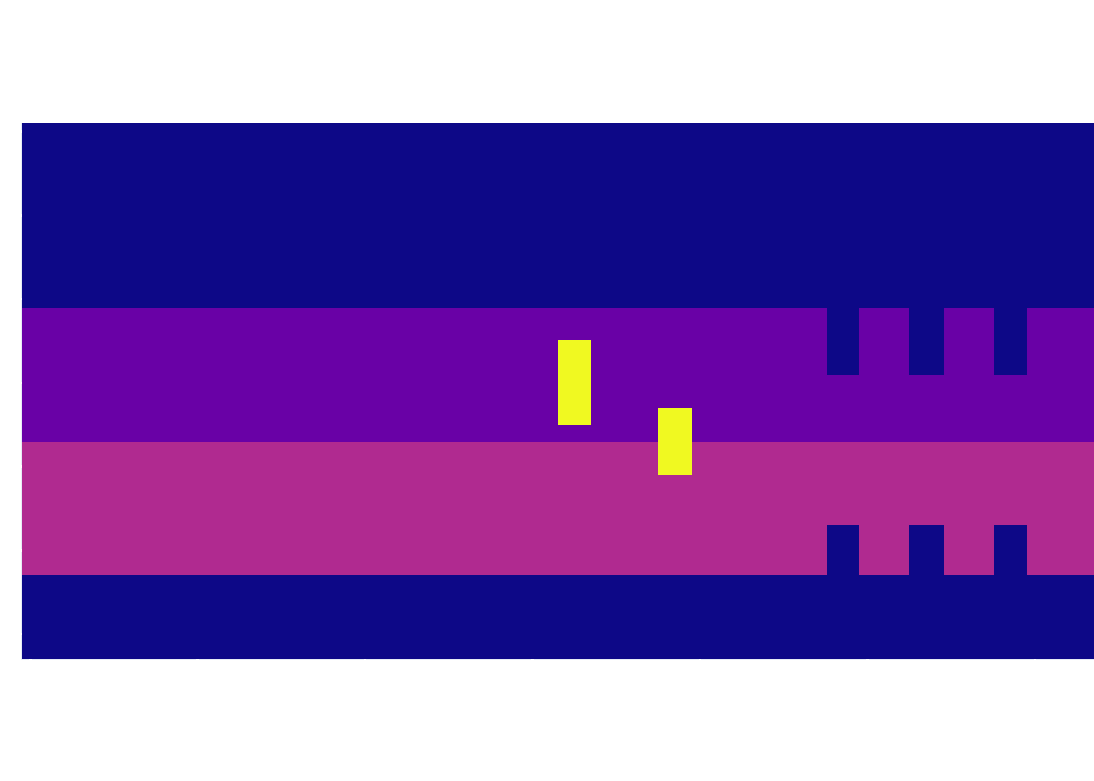
\includegraphics[scale=0.15]{images/agent_view.pdf}};
\draw[line width=0.046875cm, -latex] (5.250000, 0.35) -- (5.250000, 1.53);

%--------------------------------------------------------------------------------------------------------------------------------------------
% Policy Network
\draw[line width=0.046875cm, fill=ff_color, rounded corners=0.100000cm] (0.000000, 10.08) -- (2.500000, 10.08) -- (2.500000, 9.18) -- (0.000000, 9.18) -- cycle;
\node[text width=2.500000cm, align=center] at (1.250000, 9.68) {\footnotesize Policy \vspace{-0.3cm} \linebreak Network};

\node[text width=2.500000cm, align=center] at (0.312500, 11.580000) {$\pmb \mu$};
\node[text width=2.500000cm, align=center] at (1.250000, 11.580000) {$\pmb \sigma$};
\node[text width=2.500000cm, align=center] at (2.187500, 11.580000) {$ \hat V$};

\draw[-latex, line width=0.046875cm, rounded corners=0.200000cm] (1.250000, 10.730000) -- (0.312500, 10.730000) -- (0.312500, 11.33);
\draw[-latex, line width=0.046875cm, rounded corners=0.200000cm] (1.250000, 10.730000) -- (2.187500, 10.730000) -- (2.187500, 11.33);
\draw[line width=0.046875cm, -latex] (1.250000, 10.03) -- (1.250000, 11.33);

\draw[line width=0.046875cm, -latex] (1.250000, 6.230000) -- (1.250000, 9.23);
\draw[line width=0.046875cm, -latex] (4, 9.68) -- (2.5, 9.68);

\end{tikzpicture}
\caption[Multi-agent Transformer]{The Transformer model used in this thesis. On the right side, an ECA-ResNet processes visual input maps and outputs a vector representation. On the left side, the states of all agents $\Upsilon$ relative to the ego-agent are embedded and then fed into a Transformer encoder. The resulting $|\Upsilon|$ vectors are concatenated with the output of the convolutional pipeline. A parameter-shared \gls{mlp} policy decodes the concatenated representations, producing a distribution $(\pmb \mu, \pmb \sigma)$ and a value estimate $\hat V$ for each agent.}\label{fig:transformer}
\end{figure}
The architecture consists of two main components: First is a convolutional tower processing the visual map of the ego agent restricted to its own point of view. Note that all operations in the following description assume $3 \times 3$ kernels unless explicitly stated otherwise. After an initial convolutional layer, the image is downsampled using a pooling layer with stride $2$. This initial stage is followed by three basic convolutional blocks \cite{heDeepResidualLearning2015}, where the first convolution has stride $2$ and increases the number of filters by a factor of $2 \times$ over the output of the previous block. The second convolutional layer of each block uses stride $1$ and does not change the depth of the feature maps. All blocks use skip connections to alleviate the degradation problem \cite{heDeepResidualLearning2015}, which add the input of a block to its output. Before the block's input is added through the skip connection, an ECA-module learns global channel context \cite{wangECANetEfficientChannel2020}. Adding a channel-attention mechanism to the convolutional network is motivated by significant performance gains in applications to Go \cite{wuAcceleratingSelfPlayLearning2020}. The final component of the image processing pipeline consists of a fully convolutional head inspired by \cite{howardSearchingMobileNetV32019}. It uses two convolutional layers with $1 \times 1$ kernel size after applying an average pooling operation. The network output of the convolutional tower is a compact vector representation of the input image, denoted as $\mathbf m$.

The core component which lets the model learn interactions between a flexible number of agents is a Transformer encoder. The difference between the Transformer encoder and a decoder is that the encoder allows interactions in both directions of the sequence. The decoder on the other hand uses masking to ensure that only left-to-right dependencies are modeled\footnote{In natural language processing, this means that the encoder produces a bidirectional representation. BERT is a prominent example of such a model \cite{devlinBERTPretrainingDeep2019}. The decoder is instead used for classical language modeling, e.g. in the GPT architecture. Here the model cannot condition on future tokens, i.e. right to left dependencies \cite{devlinBERTPretrainingDeep2019}.}. Recall that an agent's numerical state $\mathbf s_i^{\text{num}} (t)$ consists of its own trajectory data as well as the relative trajectories of the other agents in the scenario (see Section~\ref{sssec:input_representation}). This can be interpreted as a sequence of objects between all of which interactions are learned by utilizing the multi-head attention mechanism. Following the steps outlined in Section~\ref{sssec:attention}, the agent trajectories are first normalized and then embedded using a single fully connected layer. This produces an $|\Upsilon| \times d_{model}$ representation matrix $\mathbf Z$, where $|\Upsilon|$ is the number of agents in the scenario. Then positional encodings are added, allowing the network to identify each agent in the sequence. In this work, learned positional embeddings are used compared to fixed sinusoidal ones \cite{devlinBERTPretrainingDeep2019}. The embedded and augmented agent trajectories are next fed into a Transformer encoder with four layers to learn bidirectional interactions between the agents. Finally, the output of the Transformer is a representation matrix $\mathbf T$ of size $|\Upsilon| \times d_{model}$.

To obtain a distribution for each agent in the scenario, each row of the matrix $\mathbf T$ is concatenated with the vector output $\mathbf m$ of the convolutional tower. This can be interpreted as a sequence of combined representations for each agent. The elements of the sequence are then fed into an \gls{mlp} policy network utilizing parameter-sharing. Reusing the network weights helps to keep the model as small as possible. In the final step, the policy outputs distribution parameters and value estimates for each agent.

The multi-agent Transformer architecture described in the previous paragraphs fulfills the requirement of being able to handle a flexible number of traffic participants. What is the intuition behind the model? Clearly an agent only receives information from its own sensors. Using itself as a model though, it can exploit the incomplete information obtained from other agents to approximate their action distributions. Of course this kind of modeling becomes coarser and coarser the further other agents are away. It is however not unlike humans make predictions about the immediate future of traffic situations. Drivers also have to plan using imperfect information, as they only perceive the road from their perspective.

The last part missing from the concept now that a network architecture has been determined is a training procedure. It is outlined in the next section.

\subsection{Training algorithm}\label{ssec:training_loop}
\begin{algorithm}[ht]
\SetAlgoLined
\begin{multicols}{2}
 Set Python, Numpy, PyTorch seeds to $S$.\\
 Initialize network parameters $\theta$ randomly.\\
 Initialize empty buffer $\mathcal D = \emptyset$.\\
 \For{$e=0$ \KwTo $E$}{
 \definecolor{shadecolor}{RGB}{0,128,0}
 \transparent{0.5}%
 \begin{shaded}
 {
 \transparent{1.0}%
 \While{$t < T$}{
    Load new network parameters $\theta$.\\
    Execute guided \gls{mcts}.\\
    Generate samples $(\mathbf s, \mathbf a, \mathbf n, \Vtarget) \sim \phat$.
  }
  }
 \end{shaded}
 \vspace{-1cm}
  \definecolor{shadecolor}{RGB}{0,0,139}
  \transparent{0.5}%
 \begin{shaded}
 {
 \transparent{1.0}%
  Store samples:\\ 
  $\mathcal D \leftarrow \mathcal D \cup \{ (\mathbf s, \mathbf a, \mathbf n, \Vtarget) \}_{t=1}^T$.\\
  \If{$|\mathcal D| > D$}{
    Remove $|\mathcal D| - D$ oldest samples.
   }
  \For{$p=0$ \KwTo $P$}{
    Draw $B$ samples $\{ (\mathbf s, \mathbf a, \mathbf n, \Vtarget) \}_{b=1}^B \sim \mathcal D$.\\
    Generate action log-probabilities $\log \pi_\theta (\mathbf a_b | \mathbf s_b)$.\\
    Generate value estimates $V_\theta (\mathbf s_b)$.\\
    Update $\theta \leftarrow \theta - \lambda \mathcal L_\theta (\mathbf a_b, \mathbf s_b)$.
  }
  }
   \end{shaded}
 }
 \columnbreak
 {
 \textbf{Algorithm components}\\
 Guided \gls{mcts} policy \phat \\
 Network policy \p\\
 Fixed size replay buffer $\mathcal D$\\ 
 ~\\
 }
 {
 \textbf{Hyperparameters}\\
 Seed $S$\\
 Replay buffer size $D$\\
 Number of Episodes $E$\\
 Number of samples $T$\\
 Number of training epochs $P$\\
 Batch size $B$\\
 Learning rate $\lambda$\\ 
 ~\\
 }
  {
 \textbf{Languages}\\
 \textcolor{cppgreen}{ \textbf{C++}}\\
 \textcolor{pyblue}{ \textbf{Python}}\\
  }
 \end{multicols}
 \caption{Guided \gls{mcts} training}
 \label{algo:training_algorithm}
\end{algorithm}
The high-level training procedure for the guided \gls{mcts} is described in Algorithm~\ref{algo:training_algorithm}. Before the first execution of the search, hyperparameters are loaded from a configuration file and used to set the seeds. Then an empty replay buffer $\mathcal D$ is constructed. The neural network parameters $\theta$ are initialized randomly at the start of the training. The algorithm then performs a data-collection and training loop for $E$ episodes.

During training, experiences are generated by executing the guided \gls{mcts} with the current network parameters $\theta$. At each stage of the search, the root node states $\mathbf s$, actions $\mathbf a$ and corresponding visitation counts $\mathbf n$ are exported\footnote{Subscripts $_0$ are omitted as only root node data is exported.}. Value targets $\Vtarget$ are obtained using Equation~\ref{eq:value_target} and saved as well. Note that the training data for all agents in the scenario is exported. This provides a regularization component by presenting the network with different ego perspectives for each scenario. More importantly, it speeds up data collection by a factor of $|\Upsilon| \times$, where $|\Upsilon|$ is the number of agents in a scenario. Since the generation of experiences is by far the most expensive computational component of the algorithm, training speed is improved significantly.

To further augment the training data, Gaussian noise is added to vehicle starting positions and scenario lane width. Given the noise standard deviations as $\sigma_{\text{lane}}, \sigma_{x}$ and $\sigma_{y}$ respectively, this results in:
\begin{align}
    w_{\text{lane}} & = \bar w_{\text{lane}} +  \epsilon_{\text{lane}}, & \epsilon_{\text{lane}}  &\sim \normal{0, \sigma_{\text{lane}}}\\
    x_i (0) & = \bar x_i (0) + \epsilon_x, & \epsilon_x & \sim \normal{0, \sigma_{x}} \\
    y_i (0) & = \bar y_i (0) + \epsilon_y, & \epsilon_y & \sim \normal{0, \sigma_{y}}~,
\end{align}
where $w_{\text{lane}}$ is the lane width and $(x_i (0), y_i (0) )$ is the starting position of agent $i$. The same quantities denoted with a bar correspond to the initial locations without noise.

Once the \gls{mcts} has generated $S$ samples, the data collection stops and all experiences are stored in the replay buffer $\mathcal D$. The buffer is using a fixed-size FIFO-queue, which is indicated in Algorithm~\ref{algo:training_algorithm} by the if-clause removing the oldest samples once the maximum size $D$ is reached. More sophisticated schemes of determining the buffer size exist, e.g. using a sublinear window function \cite{wuAcceleratingSelfPlayLearning2020} or an exponentially growing buffer \cite{anthonyThinkingFastSlow2017}. However, a fixed size queue keeps it simple and is sufficient to show the efficacy of the proposed approach.

After the generated experiences have been added to the dataset $\mathcal D$, a training loop iterates over the shuffled samples in the replay buffer $P$ times. First a batch of $B$ experiences is drawn from the buffer. The states $\mathbf s_b$ and actions $\mathbf a_b$ of the batch are used to generate action log-probabilities $\log \pi_\theta (\mathbf a_b | \mathbf s_b)$ and value estimates $V_\theta (\mathbf s_b)$ from the network. Criterion~\ref{eq:multi_agent_full} can now be evaluated by using the value targets $\hat V (\mathbf s_b)$ and visitation counts $\mathbf n_b$. The final part of a training step consists of performing a gradient descent update for the neural network parameters $\theta$.

Once the network training has concluded, a new episode $e$ is started with the updated parameters $\theta$. The training proceeds for a fixed number of steps. A high level description such as the one given above of course omits a number of implementation details. The next chapter therefore highlights the most crucial choices.






\glsresetall
\section{Implementation}
\label{sec:implementation}
The goal of this chapter is to highlight some important details in the concept outlined previously. First, the general implementation of the system is discussed with an emphasis on the utilized software frameworks. This is followed by highlighting a specific code issue observed during network training. As it turns out, it is of crucial importance how the policy standard deviation is restricted.

\subsection{System implementation}\label{ssec:system_implementation}
The overall training loop of the system described in this thesis is implemented in Python, while the \gls{mcts} itself is a C++ library. Once a run is started, a neural network is initialized from random parameters and saved to disk. PyTorch is the deep learning framework chosen for this thesis because it allows seamless interoperability between Python and C++ thanks to torchscript and the libtorch C++ library \cite{paszkePyTorchImperativeStyle}. As soon as network initialization is completed, a data collector instance is constructed from a configuration file. It employs the distributed computing framework ray \cite{moritzRayDistributedFramework2018} to start multiple instances of an \gls{mcts} ROS node \cite{quigleyROSOpensourceRobot}.

The \gls{mcts} loads the saved network parameters from the disk and runs the guided search until the scenario reaches a terminal condition. Care must be taken when training data is generated from different scenarios with possibly different numbers of agents. If all scenarios were chosen with equal probability for instance, the dataset would be biased towards scenarios with more agents. This is due to the trajectories of all agents being exported according to the training procedure in Section~\ref{ssec:training_loop}. The problem is resolved by sampling scenarios with probabilities that are inversely proportional to the number of agents $|\Upsilon_n|$ in the scenario. The probabilities can be obtained by first determining an unnormalized weight for a scenario $n$:
\begin{align}\label{eq:unnormalized_probs}
    |\Upsilon_n| \cdot w_n & =  \frac{1}{|S|} \nonumber \\
    \llap{$\Leftrightarrow$ \qquad\quad} w_n &  =  \frac{1}{|\Upsilon_n| \cdot |S|}~.
\end{align}
The intuition behind Formula~\ref{eq:unnormalized_probs} is to have scenarios weights $w_n$ which result in a uniform distribution $\frac{1}{|S|}$ when multiplied by the number agents in a scenario $|\Upsilon_n|$. A valid probability distribution can then be generated through normalization of all individual weights $w_n$ by the sum of all weights $\sum_{s=1}^S w_s$:
\begin{gather}
    P(S_n) = \frac{w_n}{\sum_{s=1}^S w_s}~,
\end{gather}
where $P(S_n)$ specifies the probability of sampling scenario $n$ for data generation.

During \gls{mcts} execution, the rollouts are replaced by a simulation policy which uses network evaluations to add both distribution parameters and value estimates to a node. Ego rewards obtained during execution of the search are normalized between $-1$ and $1$ using Formula~\ref{eq:reward_normalization}
\begin{gather}\label{eq:reward_normalization}
    \hat r = -1 + \frac{ (r - \max(r) + d) \cdot 2 }{d}~,
\end{gather}
where $r$ is the unnormalized reward given by the reward function in Section~\ref{sssec:scenario_rewards} and $d$ is the diameter of the reward interval. $\max(r)$ is the maximum obtainable reward. The used values can be found in Appendix~\ref{app:hyperparameter_settings}.

Unlike the Python framework, the libtorch C++ library does not possess a frontend for the PyTorch distributions. Therefore all policy distributions used in this work are implemented manually using Eigen3 \cite{guennebaudEigenV32010} to keep them as lightweight as possible.  After a stage of the search has finished, the root node statistics for each agent are exported in a PyTorch archive and saved on an SSD. They constitute the training data. Once enough data for an episode has been generated, the data collector terminates the \gls{mcts} runs. Subsequently, a PyTorch dataset is constructed from the $D$ newest samples, where $D$ is the size of the replay buffer. The network is then trained with stochastic gradient descent. Because storing data and training the network comprises only a fraction of the total training time these operations are implemented in Python.

If a rolling average computed from the success rate of the last three training episodes is higher than that of the previous best model, the network is saved to generate data in the next episode. When the current success rate average does not improve on the highest value, the gating test has been failed. In this case, the next batch of training experiences is still generated from the older model with the highest success rate. Nonetheless, the training proceeds with the current network and without reloading the weights.

Section~\ref{sssec:progressive_widening} has established that progressive widening is done on a per-agent basis. Since the data collection phase might use scenarios with different numbers of agents, special attention has to be paid to padding the data batches. Value targets are padded using a large negative constant $-1 \cdot 10^{10}$. On one hand, this provides direct feedback through exploding loss values in the case of bugs. On the other hand, since rewards are normalized, it is easy to generate a mask for padded values.

Agent actions and visitation counts are padded using zero values. To generate a mask for the policy and entropy loss (refer to Section~\ref{ssec:objective_function}), note that an exported action cannot have a visitation count of zero. Therefore generating a mask that removes all zero visitation counts can also be used to discard log-probabilities generated from padded actions. The last implementation detail worth discussing is significant enough to warrant its own section, which follows.

\subsection{Restricting the policy standard deviation}\label{ssec:restricting_stddev}
When learning the standard deviation $\sigma$ of a normal distribution in \gls{rl}, one usually proceeds as follows \cite{schulmanTrustRegionPolicy2017, raffinStableBaselines32019}:
\begin{enumerate}
    \item Learn the logarithm of the standard deviation $\log \sigma$ instead of restricting the learned parameter to positive ranges only.
    \item Restrain $\log \sigma$ to be in some range, e.g. an interval between $2$ and $-20$.
    \item Calculate $e^{\log \sigma}$ as standard deviation of the distribution.
\end{enumerate}
In this process, step one helps to increase training stability by allowing the learned parameter to take positive and negative values. The second step adds numerical stability to the learning by capping outliers and restricting $\log \sigma$ to prudent values. Lastly, the actual standard deviation is computed by exponentiating the learned parameter. This ensures $\sigma \geq 0$, which is needed to generate a valid normal distribution.

The technique by which $\log \sigma$ is restricted is rarely specified but of critical importance. One common approach taken is to use "\emph{clamping}" to cap the network output between interval boundaries \cite{raffinStableBaselines32019}. The code snippet below implements this in PyTorch:
\begin{lstlisting}[language=Python, deletekeywords={sum}]
log_param_min, log_param_max = self.log_param_bounds
log_std = torch.clamp(log_std, min=log_param_min, max=log_param_max)
\end{lstlisting}
\texttt{torch.clamp} simply cuts values outside the target interval off and replaces them with the minimum or maximum possible values. Another option is to use a $\tanh$ transformation to restrict the standard deviation \cite{yaratsSoftActorcriticSAC2020}:
\begin{lstlisting}[language=Python, deletekeywords={sum}]
log_std = torch.tanh(log_std)
log_std_min, log_std_max = self.log_std_bounds
log_std = log_std_min + 0.5*(log_std_max - log_std_min) * (log_std + 1)
\end{lstlisting}
Here the learned parameter is first constrained between $-1$ and $1$. Then $\log \sigma$ is rescaled and a bias term is added to achieve the desired interval boundaries.
Now that both methods have been described, the question becomes: Which one to choose? This thesis uses the clamping approach motivated by its empirical performance.
\begin{figure}
\begin{subfigure}{\textwidth}
  \centering
  \scalebox{0.7}{
  \input{images/clamped_density_maze.pdf_tex}
  }
  \caption{Density obtained through $\log \sigma$ clamping.}
  \label{fig:clamped_maze_density}
\end{subfigure}

\begin{subfigure}{\textwidth}
  \centering
  \scalebox{0.7}{
  \input{images/tanh_density_maze.pdf_tex}
  }
  \caption{Density obtained through $\log \sigma$ transformation.}
  \label{fig:tanh_maze_density}
\end{subfigure}
\caption[Different versions of restricting the policy standard deviation]{Contour histograms using different techniques to restrict the standard deviation. To generate the plots, $50000$ samples were drawn from the distribution parameters produced by the same random neural network. a) uses clamping to restrict the learned log standard deviation. As a result, the random initialization leads to exploration of the whole sample space. b) uses the $\tanh$ transformation. The resulting distribution resembles a $2D$ standard normal distribution and narrowly restricts sampling around the origin.}
\label{fig:tanh_vs_clamped_std}
\end{figure}
Figure~\ref{fig:tanh_vs_clamped_std} provides an explanation for the observed superiority of clamping. In the experiment, an identical neural network with random parameters is initialized. Then the distribution generated by these parameters is visualized by drawing $50000$ samples and plotting an approximate $2D$ density over the action space.

Analyzing the results, it becomes immediately clear why the $\tanh$ method struggles to learn: The distribution generated is centered around the origin, but with a very narrow support. The histograms in Figure~\ref{fig:tanh_maze_density} further illustrate that values outside of the interval $[-3, 3]$ are sampled with very small probability. This is problematic, as it leaves a large amount of the action space unexplored at the start of training. Using a scaled $\tanh$ transformation to cap the $\log$ standard deviation therefore inhibits learning.

Comparing the \texttt{torch.clamp} approach, it can be seen that the distribution has four modes, one in each corner of Figure~\ref{fig:clamped_maze_density}. There is however also a reasonable likelihood of generating samples from all areas of the action space. This is desirable for a random network at the start of training: It allows the algorithm to fully explore all available actions before narrowing the distribution, thereby preventing premature convergence to local optima.

For the reasons elaborated on above, all experiments in the following section use clamping instead of the $\tanh$ transformation to restrict the $\log$ standard deviation.



\glsresetall
\section{Evaluation}\label{sec:evaluation}
To evaluate the proposed approach, two scenarios are used to train models: Scenario 06 (Figure~\ref{fig:sc06}), where two agents have to merge, and scenario 08 (Figure~\ref{fig:sc08}), where two agents have to pass a bottleneck. Scenario 06 is easier and allows multiple ablation studies whereas scenario 08 can be considered more challenging\footnote{Why that is the case is disclosed in Sections~\ref{ssec:eval_baseline} and~\ref{ssec:eval_vs_mcts}.}. It should therefore provide more insights into the potential of the guided search algorithm. After introducing a baseline used for comparison, the section headers serve as guiding questions for the studies conducted in the body.

\subsection{Evaluation Metrics}\label{ssec:evaluation_metrics}
The algorithm described in the previous sections is empirically analyzed according to one main metric: the success rate. A scenario run is deemed successful if no collisions or invalid states occur. They are denoted with indicator variables $I_{\text{collision}}$ for a collision and $I_{\text{invalid}}$ for an invalid state. Recall that a state is invalid if the vehicle is not on the drivable area (refer to Section~\ref{sssec:scenario_rewards}). Additionally, if the algorithm was unable to generate actions for each agent, the run is stopped with an indicator $I_{\text{unable\_continue}}$. Therefore the success of a single run can be stated in Definition~\ref{eq:scenario_success}:
\begin{gather}\label{eq:scenario_success}
        I_{\text{success}} = \max (1 - I_{\text{collision}} - I_{\text{invalid}} - I_{\text{unable\_continue}}, 0)~.
\end{gather}
The indicator variable success is thus one if neither of the aforementioned negative events occurs. If a collision, invalid state or failed planning attempt has taken place, it is zero. Aggregating the individual scenario successes into the success rate over $N$ evaluations can be written as
\begin{gather}
    P_{\text{success}} = \frac{1}{N} \sum_{n=1}^N I^n_{\text{success}}~,
\end{gather}
where $P_{\text{success}}$ is the success rate and $I^n_{\text{success}}$ is the indicator of success for the $n$-th run. 

In this place it is worth mentioning that in \gls{rl} usually the episode reward is used to determine the learning progress. For the multi-agent driving scenarios evaluated in this thesis, the normalized cooperative reward $R$ is given as
\begin{gather}
    R = \frac{1}{T} \sum_{t=1}^T \frac{1}{|\Upsilon|} \sum_{i=1}^\Upsilon r_{i, t}~,
\end{gather}
where $r_{i, t}$ is the reward of agent $i$ at time step $t$. $r_{i, t}$ is summed over all agents and time steps in the scenario before being averaged over the number of steps $T$ in the episode as well as the agent count $|\Upsilon|$. As will be discussed in Sections~\ref{ssec:eval_vs_mcts} and ~\ref{ssec:interpretation}, using the normalized cooperative reward as measure of success is problematic.

Another metric used in the subsequent evaluation is the percentage of times an agent's desire has been fulfilled. Recall from Section~\ref{ssec:environment} that each agent has a goal state consisting of a target lane and a target velocity in longitudinal direction. How often this goal state is reached for a total number of $N$ runs can then be used as an alternative measure of success:
\begin{gather}\label{eq:desire_fulfilled}
    P_{\text{desire\_fulfilled}} = \frac{1}{N} \sum_{n=1}^N I^n_{\text{desire\_fulfilled}}~,
\end{gather}
where $I^n_{\text{desire\_fulfilled}}$ indicates that an agent's desire has been reached in the $n$-th run.

To facilitate reproducibility of the results shown in the following sections, the hyperparameters for the evaluation and training runs are stated in Appendix~\ref{app:hyperparameter_settings}. They are kept fixed across all runs unless explicitly stated otherwise. All training runs use the same network architecture which is defined in Appendix~\ref{app:network_architecture}. The seeds to initialize the random number generators for training and evaluation are specified in Appendix~\ref{app:training_seeds} and~\ref{app:evaluation_seeds}, respectively. When a trained model is evaluated, no learning occurs and its weights are kept fixed.

Now that the metric for evaluation and the training settings have been discussed, the following sections empirically analyze the capabilities of the proposed algorithm.

\subsection{The baseline}\label{ssec:eval_baseline}
When evaluating any method, it is important to select a competitive baseline as comparison. As such, the \gls{mcts} developed by \cite{kurzerDecentralizedCooperativePlanning2018} is chosen when evaluating the proposed approach. It uses several heuristics to improve its performance in low iteration settings. This is in contrast to the network-guided search which learns from tabula rasa. In the following, these heuristics are explained.

To generate new actions for progressive widening, Section~\ref{sssec:progressive_widening} refers to uniform sampling as the simplest strategy. The baseline however uses \emph{Blind Values} as an orthogonal approach to produce guided actions \cite{couetouxImprovingExplorationUpper2012, kurzerDecentralizedCooperativePlanning2018}. Action generation proceeds as follows: For each actually chosen action, first a set of candidate actions is sampled uniformly from the action space. Their blind value is calculated subsequently. It can be seen as a scoring function utilizing the statistics of already explored actions. Together with a distance measure the statistics provide an attractiveness score \cite{kurzerDecentralizedCooperativePlanning2018}. The value is high for actions far from already selected ones at the beginning of the search. With higher visitation counts, actions with higher UCT values are preferred. Blind values thus weigh exploration versus exploitation for each actually expanded action \cite{kurzerDecentralizedCooperativePlanning2018}.

As a second heuristic that is particularly useful in low iteration settings, the baseline adds a number of pre-calculated maneuvers to each newly expanded node. These maneuvers are generated by calculating actions which conform to previously determined semantic action groups \cite{kurzerDecentralizedCooperativePlanning2018}. An example action from these groups is for instance a lane change to the left while decelerating. To calculate values for the chosen maneuvers, the \gls{mcts} relies on the scenario specification \cite{kurzerDecentralizedCooperativePlanning2018}. The number of actions added this way is dependent on the search depth: If the newly expanded node is close to the root of the tree, nine pre-calculated maneuvers are added. For nodes deeper in the tree, only five basic actions are generated \cite{kurzerDecentralizedCooperativePlanning2018}.

What happens if the predetermined driving maneuvers in the last paragraph do not conform to the action bounds? In this case, the baseline \gls{mcts} \emph{ignores the constraints}. As a result, it is able to select actions which are not accessible to the \gls{rl} algorithm. Through the $\tanh$ squashed normal distribution introduced in Section~\ref{ssec:action_bounds}, the approach proposed by this thesis cannot violate the action bounds.

To make results comparable, actions are bounded for the baseline in the following evaluation. Additionally, ego reward normalization according to Equation~\ref{eq:reward_normalization} is added to produce equally scaled values. Table~\ref{tab:baseline_performance} shows how these modifications alter the baseline results. Enforcing action bounds has a negligible effect on the success rate. Interestingly, the ego reward normalization improves the baseline compared to using unnormalized rewards. A variant of the \gls{mcts} without pre-calculated maneuvers is also evaluated. Without them, the baseline is not able to solve scenarios 02, 05, 06, and 07 at all. This highlights its reliance on heuristics in low iteration settings.

Due to its higher success rate and comparable reward values over the unmodified baseline, the \textbf{Bound \& Norm} variant from Table~\ref{tab:baseline_performance} is chosen for all further evaluations. As scenarios, 06 is selected as it is solvable easily by the \gls{mcts}. This allows an evaluation of whether the guided search is able to recover the pre-calculated heuristic maneuvers. As another scenario, 08 is chosen. Here the heuristic actions are insufficient and cannot solve the task, as evidenced by the \gls{mcts} needing more iterations.

With the baseline being introduced, the focus of this work now shifts towards evaluation of the guided search approach. A starting point is a qualitative overview assessing whether the network is able to successfully prune the sample space.
\begin{landscape}
\begin{table}[h]
 \centering
 \scalebox{0.9}{
  \begin{tabular}{lcccccccccc}
    \toprule
     & \multicolumn{2}{c}{\textbf{Base}} & \multicolumn{2}{c}{\textbf{Norm}} & \multicolumn{2}{c}{\textbf{Bound}} &  \multicolumn{2}{c}{\textbf{Bound \& Norm}} & \multicolumn{2}{c}{\textbf{No pre-selection}} \\
    \textbf{Iterations} & $100$ & $200$ & $100$ & $200$ & $100$ & $200$ & $100$ & $200$ & $100$ & $200$  \\
    \textbf{Scenario} & & & & & & & & & &  \\
    \midrule
    Scenario 01 & $0.99$ & $0.98$ & \cellcolor{lightkit}$1.00$ & $0.98$ & $0.99$ & $0.98$ & \cellcolor{lightkit}$1.00$ & $0.98$ & \cellcolor{lightkit}$1.00$ & \cellcolor{lightbrown}$1.00$ \\
    Scenario 02 & $0.80$ & $0.82$ & \cellcolor{lightkit}$0.97$ & \cellcolor{lightbrown}$0.96$ & $0.80$ & $0.82$ & \cellcolor{lightkit}$0.97$ & \cellcolor{lightbrown}$0.96$ & $0.00$ & $0.00$ \\
    Scenario 03 & \cellcolor{lightkit}$1.00$ & \cellcolor{lightbrown}$1.00$ & \cellcolor{lightkit}$1.00$ & \cellcolor{lightbrown}$1.00$ & \cellcolor{lightkit}$1.00$ & \cellcolor{lightbrown}$1.00$ & \cellcolor{lightkit}$1.00$ & \cellcolor{lightbrown}$1.00$ &  \cellcolor{lightkit}$1.00$ & \cellcolor{lightbrown}$1.00$ \\
    Scenario 04 &  $0.98$ & \cellcolor{lightbrown}$1.00$ & $0.99$ & $0.99$ &  $0.98$ & \cellcolor{lightbrown}$1.00$ & $0.99$ & $0.99$ & \cellcolor{lightkit}$1.00$ & \cellcolor{lightbrown}$1.00$ \\
    Scenario 05 & $0.91$ & $0.95$ & $0.99$ & $0.98$ & $0.92$ & $0.93$ & \cellcolor{lightkit}$1.00$ & \cellcolor{lightbrown}$0.99$ & $0.00$ & $0.00$ \\
    Scenario 06 & $0.97$ & $0.97$ & \cellcolor{lightkit}$0.99$ & \cellcolor{lightbrown}$1.00$ & $0.97$ & $0.99$ & \cellcolor{lightkit}$0.99$ & \cellcolor{lightbrown}$1.00$ & $0.00$ & $0.00$ \\
    Scenario 07 & \cellcolor{lightkit}$0.08$ & \cellcolor{lightbrown}$0.12$ & $0.07$ & $0.11$ & \cellcolor{lightkit}$0.08$ & \cellcolor{lightbrown}$0.12$ & $0.07$ & $0.11$ & $0.00$ & $0.00$ \\
    Scenario 08 & $0.17$ & $0.69$ & $0.20$ & \cellcolor{lightbrown}$0.79$ & $0.17$ & $0.69$ & $0.20$ & \cellcolor{lightbrown}$0.79$ & \cellcolor{lightkit}$0.39$ & $0.49$ \\
    \midrule
    \textbf{Mean} & $0.7375$ & $0.8163$ & $0.7763$ & $0.8513$  & $0.7388$ & $0.8163$ &  \cellcolor{lightkit}$0.7775$ & \cellcolor{lightbrown}$0.8525$  & $0.4238$ & $0.4363$  \\
    \bottomrule
  \end{tabular}
  }
\caption[Baseline performance for $100$ and $200$ iterations]{Performance of the baseline \gls{mcts} for $100$ and $200$ iterations. \textbf{Norm} corresponds to normalized ego rewards according to Equation~\ref{eq:reward_normalization}. \textbf{Bound} enforces action bounds in $[-5, 5]$. The combination is denoted as \textbf{Bound \& Norm}. \textbf{No pre-selection} shows performance without expanding pre-calculated maneuvers. The best performing algorithms are shown in cyan ($100$ iterations) and brown ($200$ iterations). Ego reward normalization improves the baseline results. Not using pre-selected actions yields a performance drop-off. For all following comparisons, the \textbf{Bound \& Norm} baseline version is chosen as it performs best and produces comparable reward values.}
\label{tab:baseline_performance}
\end{table}
\end{landscape}


\subsection{Does the model work as intended?}\label{ssec:eval_pruning}
The goal of this thesis as stated in the introduction is to improve the \gls{mcts} sample efficiency through guiding the search with learned knowledge. A simple, yet effective way to qualitatively verify whether the desired phenomenon occurs or not is to visualize the network distributions.

Figure~\ref{fig:sample_space_pruning_example_06} contrasts an agent's view in scenario 06 with the output distribution of the neural network. 
\begin{figure}
\begin{subfigure}{\textwidth}
  \centering
  \scalebox{0.7}{
  \input{images/sc06_agent0_example_maps.pdf_tex}
  }
  \caption{Agent zero visual map.}
  \label{fig:sc06_example_maps}
\end{subfigure}

\begin{subfigure}{\textwidth}
  \centering
  \scalebox{0.7}{
  \input{images/sc06_agent0_example_dists.pdf_tex}
  }
  \caption{Agent zero output distribution. $x$-axis refers to longitudinal velocity change in $m/s$. $y$-axis is lateral velocity change in $m/s$.}
  \label{fig:sc06_example_dists}
\end{subfigure}
\caption[Action space pruning for scenario 06]{First three steps of scenario 06 for agent zero. In (a), the perceived visual maps are shown. It can be seen how the agent is approaching obstacles on its lane. (b) shows the distributions produced by the network for a \gls{gmm} with $3$ components. $20000$ samples are drawn to visualize the distributions. The model effectively biases the action space. The actions preferred by the network can be interpreted as decelerated lane change to the left.}
\label{fig:sample_space_pruning_example_06}
\end{figure}
The visual maps in Subplot~\ref{fig:sc06_example_maps} depict the situation: Agent zero approaches a number of obstacles on its current lane and must merge into the middle lane to avoid a crash. At the same time, agent one can be seen entering the images from above. It also desires to merge into the center.

The corresponding network distributions are shown below in Figure~\ref{fig:sc06_example_dists}. It can be seen how the \gls{gmm} effectively prunes all actions in the sample space which correspond to driving to the right. As this would lead to either driving off the road or colliding with an obstacle, the network guides the \gls{mcts} as intended. Additionally, the network shows a preference for slowing down when approaching the obstacle in the first plot of~\ref{fig:sc06_example_dists}. After that, actions are sampled over the whole longitudinal range. Through this, the agent is able to avoid the other vehicle by either accelerating or decelerating. The latter two visualizations in Graphic~\ref{fig:sc06_example_dists} indicate that the network still prefers deceleration.

A less dramatic example of the model's prediction of the action space is shown in Figure~\ref{fig:sample_space_pruning_example_10}.
\begin{figure}
\begin{subfigure}{\textwidth}
  \centering
  \scalebox{0.7}{
  \input{images/sc10_agent0_example_maps.pdf_tex}
  }
  \caption{Agent zero visual map.}
  \label{fig:sc10_example_maps}
\end{subfigure}

\begin{subfigure}{\textwidth}
  \centering
  \scalebox{0.7}{
  \input{images/sc10_agent0_example_dists.pdf_tex}
  }
  \caption{Agent zero output distribution. $x$-axis refers to longitudinal velocity change in $m/s$. $y$-axis is lateral velocity change in $m/s$.}
  \label{fig:sc10_example_dists}
\end{subfigure}
\caption[Action space pruning for scenario 08]{First three steps of scenario 08 for agent zero. In (a), the agent is approaching the bottleneck while noticing the other vehicle. (b) The network distribution biases sampling towards a slight left turn to avoid the obstacles. To avoid a collision with the simultaneously merging other agent, all longitudinal actions are still allowed. $20000$ samples are drawn to visualize the distributions.}
\label{fig:sample_space_pruning_example_10}
\end{figure}
Here agent zero has to avoid obstacles on both lanes as well as another vehicle while driving into the bottleneck. The corresponding maps are depicted in Illustration~\ref{fig:sc10_example_maps}. Note that scenario 08 is more narrow compared to scenario 06: It only has two lanes instead of three.

The network distributions visualized in Figure~\ref{fig:sc10_example_dists} show a slight preference towards driving left. This is needed to avoid the obstacles. However, both acceleration and deceleration are permitted with no obvious inclination visible. The agent therefore stays flexible and can avoid the other vehicle by either slowing down or accelerating.

To further evaluate the proposed approach qualitatively, Figure~\ref{fig:trajectories_sc10} visualizes $20$ trajectories for each agent in scenario 08.
\begin{figure}
\begin{subfigure}{\textwidth}
  \centering
  \scalebox{0.7}{
  \input{images/trajectories_agent0.pdf_tex}
  }
  \caption{Agent zero trajectories.}
  \label{fig:trajectories_agent0}
\end{subfigure}

\begin{subfigure}{\textwidth}
  \centering
  \scalebox{0.7}{
  \input{images/trajectories_agent1.pdf_tex}
  }
  \caption{Agent one trajectories.}
  \label{fig:trajectories_agent1}
\end{subfigure}
\caption[Agent trajectories for scenario 08]{$20$ trajectories using $100$ iterations for each agent in scenario 08. Seeds are fixed, resulting in the same starting positions (denoted as red dots). Guided search is using a \gls{gmm} with three components. The plots show how both agents are able to navigate through the bottleneck without colliding more often when using the guided search. This contrasts with the pure \gls{mcts} approach, where the vehicles crash when driving into the center more regularly. }
\label{fig:trajectories_sc10}
\end{figure}
$100$ \gls{mcts} iterations are used for both the baseline as well as the guided search. The seeds are kept fixed such that the starting positions are the same for both approaches. They are marked with red dots. Obstacle positions and lane width are not randomized for visualization purposes.

Both plots show immediately how the learning based approach completes more runs than the baseline \gls{mcts}. The pair of agents passes through the middle while at the same time avoiding a collision. Their trajectories are both close to the center line between the lanes, indicating that they pass the bottleneck consecutively.

On the other hand, Figure~\ref{fig:trajectories_agent0} already shows clearly how agent zero is not able to avoid the obstacles and the other agent at the same time. Almost half of its trajectories end in the area to the left of the first obstacle. A pass of the bottleneck only succeeds four times for the baseline.

The visualizations in this section have shown that the network is able to successfully guide the search. Next, the choice of \gls{mcts} selection policy is discussed.


\subsection{Which selection policy to choose?}\label{ssec:eval_of_final_selection}
In Section~\ref{sssec:uct}, two strategies for selecting the action to be executed in the environment are introduced: selection of the action with the highest visitation count and selection of the action with the highest action value. The choice in the \gls{uct} algorithm is usually the former \cite{browneSurveyMonteCarlo2012}.

Which strategy is best for cooperative autonomous driving is not immediately obvious. Therefore a short empirical evaluation is conducted to find the best approach. 
\begin{figure}[h]
	\centering
	\captionsetup{justification=centering}
	\scalebox{0.9}{
    \input{images/sc06_final_selection_success.pdf_tex}
    }
	\caption[Training success for different selection policies]{Training success in scenario 06 using different \gls{mcts} selection policies. Both runs use $50$ iterations and the same three seeds. Selecting the action with the highest action value yields a higher success rate.}
\label{fig:final_selection_shaded}
\end{figure}
Figure~\ref{fig:final_selection_shaded} shows the training progress of both selection strategies in scenario 06 for $50$ iterations. In contrast to the literature \cite{browneSurveyMonteCarlo2012}, selecting the action with the highest action value seems to outperform selecting the most visited action.

\begin{figure}[h]
	\centering
	\captionsetup{justification=centering}
	\scalebox{0.9}{
    \input{images/sc06_selection_success_matrix.pdf_tex}
    }
	\caption[Evaluation success for different selection policies]{Training success in scenario 06 using different \gls{mcts} selection policies. Both models are trained using $50$ iterations. Selecting the action with the highest action value yields a higher success rate for lower iterations. Results are averaged for three models.}
\label{fig:final_selection_matrix}
\end{figure}
Matrix~\ref{fig:final_selection_matrix} further examines the learned models in an evaluation setting.
Overall, selecting the action with the maximum action value outperforms selection based on visitation counts with a mean success rate of $0.7686$ to $0.6971$. The difference mainly stems from low iteration settings, particularly for $5$, $10$ and $50$ iterations. For higher iteration values as well as $25$ iterations, the maximum visitation selection has a marginally higher success rate. Interestingly, the baseline is stronger than both learned models. Its high success percentage using just $5$ iterations confirms that the heuristic maneuvers are good enough to solve some scenarios outright.

\begin{table}[h]
 \centering
 \scalebox{0.8}{
  \begin{tabular}{llcccccccc}
    \toprule
    & \textbf{Iterations} & $5$ & $10$ & $25$ & $50$ & $100$ & $200$ & $400$ & \textbf{Mean}\\
    \textbf{Selection} & \textbf{Metric} & & & & & & & \\
    \midrule
    \multirow{3}{*}{\textbf{Max value}} & \textbf{Success} & \cellcolor{lightkit}$0.3967$  & \cellcolor{lightkit}$0.5533$  &  $0.6767$  &\cellcolor{lightkit}$0.8467$  & \cellcolor{lightkit}$0.9567$  & $0.9700$  &   $0.9800$ & \cellcolor{lightkit}$\mathbf{0.7686}$ \\
    & \textbf{Reward} & \cellcolor{lightkit}$0.2213$ & \cellcolor{lightkit}$0.2366$ & \cellcolor{lightkit}$0.2554$  & \cellcolor{lightkit}$0.2738$ & \cellcolor{lightkit}$0.2905$ & \cellcolor{lightkit}$0.2951$ & \cellcolor{lightkit}$0.3008$ & \cellcolor{lightkit}$\mathbf{0.2676}$ \\
    & \textbf{Desire} & $0.0000$  & $0.0000$  &  $0.0000$ &  $0.0000$ & \cellcolor{lightkit}$0.0033$  &  \cellcolor{lightkit}$0.0033$ & $0.0033$ & $\mathbf{0.0014}$ \\
    \multirow{3}{*}{\textbf{Max visits}} & \textbf{Success}  &   $0.1300$ &  $0.4200$  & \cellcolor{lightkit}$0.6900$    &  $0.7433$  &  $0.9233$  & \cellcolor{lightkit}$0.9833$  & \cellcolor{lightkit}$0.9900$ & $\mathbf{0.6971}$ \\
    & \textbf{Reward} &  $0.1514$  &  $0.2104$  &  $0.2511$ &  $0.2629$ &   $0.2865$ & $0.2942$  & $0.3001$ & $\mathbf{0.2509}$ \\
    & \textbf{Desire} & $0.0000$  & $0.0000$  &  $0.0000$  &  $0.0000$ &  $0.0000$  &   $0.0000$ & \cellcolor{lightkit}$0.0200$ & \cellcolor{lightkit}$\mathbf{0.0029}$ \\
    \bottomrule
  \end{tabular}
  }
\caption[Final selection performance in scenario 06]{Performance of different selection policies in scenario 06. Using the maximum action value as criterion outperforms selecting the most visited action in four out of seven settings. Final selection based on visitation counts has a slightly higher success rate for $25$, $200$ and $400$ iterations.}
\label{tab:selection_performance}
\end{table}
The difference between both guided search models is expounded by Table~\ref{tab:selection_performance}. In addition to the higher average success rate, maximum value selection also has the highest cooperative reward values for each iteration setting. As the number of iterations increases, the difference between both models narrows. For the rate of fulfilled desires, both maximum action value and maximum visitation count are close to zero for all settings.

Now that the choice of final selection policy has been evaluated, the next section discusses the performance of guided search versus the baseline in detail. Due to its higher mean success rate, the maximum action value policy is chosen for all following evaluations.


\subsection{How well does the learned model perform versus pure MCTS?}\label{ssec:eval_vs_mcts}
The success rate visualization of different selection policies in the last section (Figure~\ref{fig:final_selection_matrix}) shows the baseline outperforming the learned models. This raises an interesting question: Are there scenarios where the guided search exceeds the success rate of the baseline and vice versa?

Looking at the training success in Plot~\ref{fig:train_success_shaded} first, one can see how for scenario 06 the model is able to approximate the baseline performance only late during the run. 
\begin{figure}[h]
	\centering
	\captionsetup{justification=centering}
	\scalebox{0.9}{
    \input{images/sc06_sc10_train_shaded.pdf_tex}
    }
	\caption[Training plots for different scenarios]{Training progress for scenarios 06 and 08. Models are trained over three seeds using $200$ iterations. Error bands show one standard deviation. The success rate of the pure \gls{mcts} baseline for the same number of iterations is shown as dotted line.}
\label{fig:train_success_shaded}
\end{figure}
This is not surprising because the baseline completely solves the task for $200$ iterations. For scenario 08, the guided search exceeds the performance of the \gls{mcts} at around episode $65$ and continues to improve upon it.

A closer look at Table~\ref{tab:sc10_performance} confirms the hypothesis for scenario 08: The learned models guide the search effectively, yielding a higher success and desires fulfilled rate than the baseline in all iteration settings.
\begin{table}[h]
 \centering
 \scalebox{0.8}{
  \begin{tabular}{llcccccccc}
    \toprule
    & \textbf{Iterations} & $5$ & $10$ & $25$ & $50$ & $100$ & $200$ & $400$ & \textbf{Mean}\\
    \textbf{Model} & \textbf{Metric} & & & & & & \\
    \midrule
    \multirow{3}{*}{\textbf{GMM 3}} & \textbf{Success} & \cellcolor{lightkit}$0.3000$ & \cellcolor{lightkit}$0.4967$ & \cellcolor{lightkit}$0.6833$ & \cellcolor{lightkit}$0.8267$ & \cellcolor{lightkit}$0.8300$ & \cellcolor{lightkit}$0.9433$ & \cellcolor{lightkit}$0.9500$ & \cellcolor{lightkit}$\mathbf{0.7186}$ \\
    & \textbf{Reward} & $0.2779$ & $0.2954$ & $0.3119$ & $0.3205$ & $0.3276$ & $0.3341$ & $0.3367$ & $\mathbf{0.3149}$  \\
    & \textbf{Desire} & \cellcolor{lightkit}$0.0067$ & \cellcolor{lightkit}$0.0200$ & \cellcolor{lightkit}$0.0567$ & \cellcolor{lightkit}$0.1767$ & \cellcolor{lightkit}$0.1333$ & \cellcolor{lightkit}$0.2900$ & \cellcolor{lightkit}$0.3833$ & \cellcolor{lightkit}$\mathbf{0.1524}$ \\
    \multirow{3}{*}{\textbf{Baseline}} & \textbf{Success} & $0.0200$ & $0.0100$ & $0.0200$ & $0.0900$ & $0.2000$ & $0.7900$ & $0.8700$ & $\mathbf{0.2857}$ \\
    & \textbf{Reward} & \cellcolor{lightkit}$0.6738$ & \cellcolor{lightkit}$0.6430$ &  \cellcolor{lightkit}$0.6404$ & \cellcolor{lightkit}$0.6096$ & \cellcolor{lightkit}$0.6145$ & \cellcolor{lightkit}$0.6255$ & \cellcolor{lightkit}$0.6238$ & \cellcolor{lightkit}$\mathbf{0.6330}$  \\
    & \textbf{Desire} & $0.0000$ & $0.0100$ & $0.0000$ & $0.0000$ & $0.0002$ & $0.0002$ & $0.1000$ & $\mathbf{0.0214}$ \\
    \bottomrule
  \end{tabular}
  }
\caption[Scenario 08 performance versus the baseline]{Performance of the \gls{gmm} $3$ model versus the baseline in scenario 08. The best value is shaded in cyan. Using guided search outperforms the pure \gls{mcts} baseline in both success and desires fulfilled percentage. The difference is particularly stark in low iteration settings. It is noteworthy that the \gls{mcts} consistently produces runs with higher reward despite a lower success rate. For the guided search, the results of three models are averaged.}
\label{tab:sc10_performance}
\end{table}
The difference is particularly noticeable below $200$ iterations. At $100$ \gls{mcts} traces, the guided search succeeds in $83.00 \%$ of runs compared to only $20.00 \%$ for the baseline. Starting at $200$ iterations, the success rate for the baseline makes a jump and closes the gap between both approaches. Using a learned network however is still superior, which is also reflected in terms of the average success rate at $0.7186$ compared to $0.2857$.

The results described above also transfer to the rate of fulfilled desires. This should come as no surprise, as an agent is only able to reach its target state if it stays on the road and does not crash. The overall average rate of desires fulfilled across all iterations is $0.1524$ for the guided search versus $0.0214$ for the baseline.

Interestingly, the results of the previously examined evaluation metrics do not carry over to the normalized cooperative reward. Here the baseline strongly outperforms the guided search by more than a factor of $2 \times$ on average. The results for $5$ iterations especially raise questions. At this setting, the baseline achieves its highest cooperative reward despite a success rate of only $2 \%$ and no desires fulfilled.

The outcomes are flipped regarding the detailed evaluation results of scenario 06 in Table~\ref{tab:sc06_performance}. Here the baseline posts stronger results compared to the guided search in all iteration settings.
\begin{table}[h]
 \centering
 \scalebox{0.8}{
  \begin{tabular}{llcccccccc}
    \toprule
    & \textbf{Iterations} & $5$ & $10$ & $25$ & $50$ & $100$ & $200$ & $400$ & \textbf{Mean}\\
    \textbf{Model} & \textbf{Metric} & & & & & & & \\
    \midrule
    \multirow{3}{*}{\textbf{GMM 3}} & \textbf{Success} &  $0.4367$ &  $0.5733$ & $0.7133$  & $0.8533$  & $0.9467$  & $0.9900$  & $0.9933$ & $\mathbf{0.7867}$ \\
    & \textbf{Reward} & $0.2168$  &  $0.2345$ & $0.2564$  &  $0.2755$ & $0.2901$  & $0.2986$  & $0.3045$ & $\mathbf{0.2681}$ \\
    & \textbf{Desire} & $0.0000$  &  $0.0000$ & $0.0000$  &  $0.0000$ & $0.0000$  & $0.0000$  & $0.0000$ & $\mathbf{0.0000}$ \\
    \multirow{3}{*}{\textbf{Baseline}} & \textbf{Success}  & \cellcolor{lightkit}$0.8700$  & \cellcolor{lightkit}$0.9600$ &  \cellcolor{lightkit}$1.0000$   &  \cellcolor{lightkit}$0.9900$  & \cellcolor{lightkit}$0.9900$  &  \cellcolor{lightkit}$1.0000$ & \cellcolor{lightkit}$1.0000$ & \cellcolor{lightkit}$\mathbf{0.9729}$ \\
    & \textbf{Reward} & \cellcolor{lightkit}$0.5798$  & \cellcolor{lightkit}$0.4976$  & \cellcolor{lightkit}$0.4943$  & \cellcolor{lightkit}$0.4633$ & \cellcolor{lightkit}$0.4791$  & \cellcolor{lightkit}$0.5126$ & \cellcolor{lightkit}$0.5157$ & \cellcolor{lightkit}$\mathbf{0.5060}$ \\
    & \textbf{Desire} &  $0.0000$ & \cellcolor{lightkit}$0.0200$ & \cellcolor{lightkit}$0.0100$  & \cellcolor{lightkit}$0.0300$ &  $0.0000$  &  $0.0000$  &  $0.0000$ & \cellcolor{lightkit}$\mathbf{0.0086}$ \\
    \bottomrule
  \end{tabular}
  }
\caption[Scenario 06 performance versus the baseline]{Performance of the \gls{gmm} $3$ model versus the baseline in scenario 06. The best value is denoted in cyan. Pure \gls{mcts} outperforms the $200$ iteration model in all regards. The difference is particularly noteworthy in medium iteration settings ($10, 25, 50, 100$).} Three models are averaged for the guided search.
\label{tab:sc06_performance}
\end{table}
$25$ iterations are already enough for it to solve the task with $100\%$ or $99\%$ success. This is consistent with the findings of Section~\ref{ssec:eval_baseline}, which report that the pre-calculated maneuvers are enough to succeed in scenario 06. While the learned model is able to recover the knowledge added through the heuristic, it needs $200$ iterations to do so.

The results described for the success rate also carry over to the other evaluation metrics. It is noteworthy that neither the baseline nor the guided search are able to achieve a percentage of desires fulfilled higher than $3\%$. As for the cooperative reward, the baseline substantially outperforms the guided search similar to scenario 08. However, the results fluctuate without apparent relationship to the success rate.
\begin{table}[h]
 \centering
 \scalebox{0.9}{
  \begin{tabular}{lcccc}
    \toprule
    \textbf{Model} & Runs & Iterations & Success & Wall clock \\
    \midrule
    GMM 3 & $100$ & $50$ & $0.8400$ & $49s$ \\
    Baseline & $100$ & $400$ & $0.8700$ & $57s$ \\
    \bottomrule
  \end{tabular}
  }
\caption[Scenario 08 wall clock time performance]{The guided search approach is competitive with the baseline using eight times less iterations and $8s$ less wall clock time.}
\label{tab:wall_clock_performance_sc08}
\end{table}
Another important measure to look at --- particularly important for potential real-world deployment --- is the wall clock time. Tables~\ref{tab:wall_clock_performance_sc08} and~\ref{tab:wall_clock_performance_sc06} report the results. In scenario 08, the guided search achieves a similar success rate to the baseline with $8 \times$ less iterations. Due to the reduced number of planning traces, it is competitive in terms of wall clock time and even slightly faster. On scenario 06 in comparison, the learned model needs $100$ iterations to be as successful as the plain \gls{mcts}\footnote{The comparison is made between values within tables. The wall clock time between tables is not comparable due to different background workloads on the servers.}.
\begin{table}[h]
 \centering
 \scalebox{0.9}{
  \begin{tabular}{lcccc}
    \toprule
    \textbf{Model} & Runs & Iterations & Success & Wall clock \\
    \midrule
    GMM 3 & $100$ & $100$ & $0.9900$ & $2m43s$ \\
    Baseline & $100$ & $100$ & $0.9900$ & $4s$ \\
    \bottomrule
  \end{tabular}
  }
\caption[Scenario 06 wall clock time performance]{The guided search approach performs the same in terms of success percentage compared to the baseline. It requires the same number of iterations which results in non-competitive wall clock time due to the slowness of network evaluations.}
\label{tab:wall_clock_performance_sc06}
\end{table}
This results in planning that is orders of magnitude slower than the baseline. The reason for these findings lies in the computational cost of network evaluations. Profiling the code reveals that the guided search spends around $48\%$ of its runtime performing neural network inference.

Lastly, Section~\ref{ssec:network_architecture} describes how the networks can use the imperfect information gained from only one agent's point of view to plan for other agents as well. The results for the corresponding evaluations are visualized in Figures~\ref{fig:sc_10_vs_baseline} and~\ref{fig:sc_06_vs_baseline}.
\begin{figure}
\begin{subfigure}{.5\textwidth}
  \centering
  \scalebox{0.5}{
  \input{images/sc06_pov_success_matrix.pdf_tex}
  }
  \caption{Success rates for different points of view.}
  \label{fig:sc06_success_matrix}
\end{subfigure}
\begin{subfigure}{.5\textwidth}
  \centering
  \scalebox{0.5}{
  \input{images/sc06_pov_desire_matrix.pdf_tex}
  }
  \caption{Desires fulfilled for different points of view.}
  \label{fig:sc06_desire_matrix}
\end{subfigure}
\caption[Success rate and desires fulfilled in scenario 06]{The two matrices show the model performance depending on which agent is using the network in scenario 06. In (a), the success percentage is shown. (b) depicts the percentage of desires fulfilled. Planning from one agent's point of view shows similar performance compared to planning for both agents. An average of three models is shown for the guided search.}
\label{fig:sc_06_vs_baseline}
\end{figure}
For the success rate, the findings are very similar for all points of view. Using only the visual map for a single agent is usually within a bound of three percentage points higher or lower compared to using maps for both agents. This results in comparable average success rates when utilizing all maps ($0.7867$) versus only agent one's map ($0.7871$) in scenario 06. There is a slight drop-off when using agent zero's visual input only with $0.7714$.

The only outlier in scenario 08 occurs when using $100$ iterations, where planning from agent zero's point of view is more successful by four percentage points compared to both agents. Apart from that, the average success across iterations is remarkably stable: $0.7186$ for both compared to $0.7186$ (agent zero) and $0.7119$ (agent one).

When looking at the percentage of desires fulfilled, it stands out that in scenario 06 the learned models are not able to achieve values above zero with one exemption. The baseline has similarly low percentages with exceptions for $10$, $25$ and $50$ iterations.
\begin{figure}
\begin{subfigure}{.5\textwidth}
  \centering
  \scalebox{0.5}{
  \input{images/sc10_vs_baseline_success_heatmap.pdf_tex}
  }
  \caption{Success rates for different points of view.}
  \label{fig:sc10_success_matrix}
\end{subfigure}
\begin{subfigure}{.5\textwidth}
  \centering
  \scalebox{0.5}{
  \input{images/sc10_vs_baseline_desire_heatmap.pdf_tex}
  }
  \caption{Desires fulfilled for different points of view.}
  \label{fig:sc10_desire_matrix}
\end{subfigure}
\caption[Success rate and desires fulfilled in scenario 08]{The two matrices show the model performance depending on which agent is using the network in scenario 08. In (a), the success percentage is shown. (b) depicts the percentage of desires fulfilled. Using only a single agent's point of view is competitive with utilizing maps from both agents. Guided search outperforms the baseline for all settings and metrics. Three models are averaged for the guided search results.}
\label{fig:sc_10_vs_baseline}
\end{figure}

The results are more interesting for scenario 08, where fluctuations for the rate of desires fulfilled can be found starting at $25$ iterations. Using only agent zero's map performs noticeably better for $100$ \gls{mcts} traces. Both agent's point of view is more successful at $25$ and $50$ iterations. Overall however, the mean percentage of desires fulfilled hovers around $15 \%$ with $15.24 \%$ desires fulfilled when using all visual maps compared to $15.10 \%$ and $15.62 \%$ for agent zero and agent one, respectively. The baseline is not competitive at only $2.14 \%$.

\clearpage

\subsection{How important is the number of iterations?}\label{ssec:eval_of_hyperparameters}
For approaches that combine \gls{rl} with search, there is a trade-off between time allocated to the learning component of the algorithm and time allocated to the planning component \cite{moerlandThinkTooFast2020}. In the context of this thesis, planning corresponds to the number of \gls{mcts} iterations used during training. What number works best is not immediately obvious and therefore evaluated in the context of scenario 06.

Figure~\ref{fig:iter_success_shaded} shows the training progress for $50$, $100$ and $200$ iterations.
\begin{figure}[h]
	\centering
	\captionsetup{justification=centering}
	\scalebox{0.9}{
    \input{images/sc06_iteration_success.pdf_tex}
    }
	\caption[Training plots for different iterations]{Training progress with different iteration numbers. The $200$ iteration model learns in fewer episodes than both other models. Using $100$ iterations approaches a similar level of success as using $200$. For all models, three seeds are trained and one standard deviation is shown.}
\label{fig:iter_success_shaded}
\end{figure}
While all models successfully improve over the course of the episodes, the network trained with $200$ iterations exhibits the highest success rate. This is unsurprising, as more time spent in \gls{mcts} searches should not only improve the quality of the action selected in the environment but also produce enhanced training targets.

Delving deeper into the issue, Matrix~\ref{fig:iter_success_matrix} reveals an interesting dynamic: Despite being trained with a smaller time budget, the $100$ iteration model outperforms the one trained with $200$ iterations.
\begin{figure}[h]
	\centering
	\captionsetup{justification=centering}
	\scalebox{0.6}{
    \input{images/sc06_iteration_success_matrix.pdf_tex}
    }
	\caption[Evaluation results for different iterations]{Evaluation of models trained with different iteration numbers. The model using $100$ iterations performs best for medium iteration values. In high iteration settings, the networks show similar performance. All results are averaged over three models.}
\label{fig:iter_success_matrix}
\end{figure}
The phenomenon is especially noticeable when using a medium number of \gls{mcts} traces ($10$, $25$ and $50$). Both the $100$ as well as the $200$ iteration networks are superior when compared to the $50$ iteration model.

\begin{table}[h]
 \centering
 \scalebox{0.9}{
  \begin{tabular}{lcccc}
    \toprule
    \textbf{Iterations} & $50$ & $100$ & $200$ \\
    \midrule
    Wall clock & $8h53m$ & $14h28m$ & $32h11m$  \\
    Mean success & $0.7686$ & $0.7933$ & $0.7867$ \\
    \bottomrule
  \end{tabular}
  }
\caption[Training wall clock time for different iterations]{Wall clock times for different training iteration numbers in scenario 06. The mean evaluation success rate is shown below. The model using $100$ iterations has a higher evaluation success rate than both $50$ and $200$ iterations.}
\label{tab:wall_clock_iter}
\end{table}
Table~\ref{tab:wall_clock_iter} reports the mean success rates across all settings together with the wall clock time needed for the training.
It confirms the findings of the matrix plot, where the $100$ iteration model performs best. When looking at the wall clock time, it takes roughly $1.6 \times$ as long to train as the $50$ iteration model. The network trained using $200$ \gls{mcts} traces takes another $2.2 \times$ longer compared to using $100$ traces. Larger models are not trained due to the computational resources required.

After this short evaluation of the number of iterations, the next section tackles an important question regarding the policy distribution: How many mixture components are needed to properly guide the search?

\subsection{How many mixture components are needed?}\label{ssec:eval_of_components}
As noted in Section~\ref{sssec:mixtures}, a \gls{gmm} has the theoretical ability to approximate any distribution. Using a mixture model however introduces an additional hyperparameter in the number of components $K$. On one hand, having more components is desirable as it results in a more expressive model. On the other hand, it might also degrade performance or destabilize the training.

Therefore it is sensible to perform an empirical analysis to determine the optimal number of components. The training results for different $K$ in scenario 08 are shown in Figure~\ref{fig:component_trainings}. 
\begin{figure}[h]
	\centering
	\captionsetup{justification=centering}
	\scalebox{0.9}{
    \input{images/training_plots_components.pdf_tex}
    }
	\caption[Training for different numbers of components]{Training plots for models with different numbers of components $K$ in scenario 08. The Gaussian policy performs subpar compared to using a mixture model. Runs are averaged over the same $3$ seeds on Scenario 08 with one standard deviation shown.}
\label{fig:component_trainings}
\end{figure}
For each setting, three runs are executed with the same three seeds each. The error bands show one standard deviation from the mean. It can be seen clearly that a policy parameterized by only a normal distribution has a noticeably lower success rate than the mixture models. This is an indicator that a single normal distribution is not enough to fit a proper model. When increasing the number of components, no distinguishable difference in the training can be observed.

Looking at the evaluation results, a \gls{gmm} with $K=3$ shows slightly improved performance compared to the other two mixture models.
\begin{figure}
\begin{subfigure}{.5\textwidth}
  \centering
  \scalebox{0.5}{
  \input{images/comp_success_heatmap.pdf_tex}
  }
  \caption{Success rates for different $K$.}
  \label{fig:comp_success_matrix}
\end{subfigure}
\begin{subfigure}{.5\textwidth}
  \centering
  \scalebox{0.5}{
  \input{images/comp_desire_heatmap.pdf_tex}
  }
  \caption{Desires fulfilled for different $K$.}
  \label{fig:comp_desire_matrix}
\end{subfigure}
\caption[Evaluation for different numbers of components]{Desires fulfilled and success percentage for different numbers of components $K$ in scenario 08. (a) shows the success rate, where the mixture models substantially outperform a single normal distribution. All learned models are superior to the baseline. These results are also reflected in the percentage of desires fulfilled (b). An average over three models is used except for the baseline.}
\label{fig:comp_matrix_plots}
\end{figure}Plot~\ref{fig:comp_matrix_plots} shows the data for all evaluations. $100$ runs with fixed seeds are performed for each iteration setting and averaged over three models for each $K$ to obtain the results.
Matrix~\ref{fig:comp_success_matrix} shows a slightly higher success rate for the \gls{gmm} with three components. Its mean success rate is $0.7186$ versus $0.7052$ for $K=4$ and $0.6948$ for the \gls{gmm} $2$. Additionally, it possesses the highest success rate in four out of seven iteration settings. All models outperform the baseline and all mixture models outperform a single normal distribution. Lastly, it is noteworthy that a \gls{gmm} with four components shows slightly better results than using two components.

The findings regarding the success rate carry over to the percentage of desires fulfilled in Matrix~\ref{fig:comp_success_matrix}. Again, all learned models show stronger results than the baseline and the normal distribution cannot compete with mixture models. The \gls{gmm} with three components outperforms the other networks, particularly for $50$ and $200$ iterations. This results in the highest mean desires fulfilled percentage of $0.1524$ versus $0.1419$ for the \gls{gmm} $2$ and $0.1410$ for $K=4$.

Harnessing the results from the previous paragraphs, all other models are trained using a \gls{gmm} with three components. The evaluation of whether centralized training improves the learning process therefore only uses $K=3$ in the following section.

\subsection{What is the effect of centralized training?}\label{ssec:eval_of_centralized_training}
In Section~\ref{sssec:central_plan_decentral_ex}, the \emph{Centralized Training with Decentralized Execution} paradigm is introduced as a technique to stabilize training performance.
\begin{figure}[h]
	\centering
	\captionsetup{justification=centering}
	\scalebox{0.6}{
    \input{images/sc06_decentralized_success_matrix.pdf_tex}
    }
	\caption[Centralized training versus decentralized training]{Model evaluations for centralized training and decentralized training on scenario 06. Both were trained using $100$ iterations. Centralized training slightly outperforms decentralized training. Using centralized value estimates at evaluation time (\emph{Central eval}) shows no success rate gains over decentralized evaluation. Plain \gls{mcts} is superior to both models.}
\label{fig:centralized_decentralized_matrix}
\end{figure}
Figure~\ref{fig:centralized_decentralized_matrix} shows the evaluation results of models differing in their usage of centralized value targets.

During the training and evaluation of the guided search approach, all agents make decisions from their own point of view. In particular, they calculate value estimates and distributions conditioned on their own state. This produces an accurate ego reward estimate as both numerical states and a visual map is available to each agent. Centralized training in the context of this thesis refers to using only the ego reward estimates during training. An ego agent's reward estimates for the other vehicles are discarded, as they rely on incomplete information. After all, the ego agent only has a map from its own point of view at its disposal.

Centralized value targets minimally increase the mean success percentage by $0.76$ percentage points ($0.7857$ to $0.7933$). The increase is not consistent across iterations. Furthermore, adding centralized value targets at evaluation time yields an even smaller benefit of $0.05$ percentage points. The final mean success rate improves from $0.7933$ t $0.7938$.

After centralized value targets have been shown to not be a key component to network training, the next ablation study examines whether learned value targets are needed at all.

\subsection{How important are the learned value estimates?}\label{ssec:eval_of_value_targets}
Both AlphaZero as well as the A0C algorithm on which this thesis is based use a network architecture with two heads. One head learns a policy, whereas the other head learns value estimates for environment states \cite{silverGeneralReinforcementLearning2018, moerlandA0CAlphaZero2018}. This architecture has shown improved performance compared to separate networks for each task \cite{silverMasteringGameGo2017}. In the application to Go, truncating potentially long rollouts is reasonable, especially since a strong rollout policy can be expensive to compute \cite{silverMasteringGameGo2016}.

Compared to learned value targets, using rollouts may be able to accelerate training progress by improving early state value estimates. The simulation policy used in the context of this thesis is able to choose from five basic actions: acceleration and deceleration without lateral movement, lane change to the left or right without change in longitudinal velocity and "doing nothing" (no velocity change in either direction). The choice between these actions is made by uniform sampling \cite{kurzerDecentralizedCooperativePlanning2018}.

In an evaluation of whether the rollout policy described above is able to improve performance over learned value estimates, the first step comprises looking at the training progress. It is depicted in Figure~\ref{fig:sc10_rollout_success}.
\begin{figure}
\begin{subfigure}{.5\textwidth}
  \centering
  \scalebox{0.55}{
  \input{images/sc10_rollout_success.pdf_tex}
  }
  \caption{Training success.}
  \label{fig:sc10_rollout_success}
\end{subfigure}
\begin{subfigure}{.5\textwidth}
  \centering
  \scalebox{0.55}{
  \input{images/sc10_rollout_explained_var.pdf_tex}
  }
  \caption{Explained variance}
  \label{fig:sc10_rollout_explained_var}
\end{subfigure}
\caption[Rollout training and explained variance]{(a) shows the training success of using \gls{mcts} rollouts versus learned value targets in scenario 08. Both models perform similarly. (b) depicts the explained variance. The rollout model converges faster and to a higher value. Both plots show one standard deviation error bands for three seeds.}
\label{fig:rollout_plots}
\end{figure}
Both value estimation methods show almost identical performance during the training.

A quantity which can be helpful for evaluating whether successful value learning occurs is the coefficient of determination or $R^2$. It is given in Definition~\ref{eq:explained_var} and explains how well predictions $\hat y_i$ explain the variation of a target variable $y_i$ \cite{weisbergAppliedLinearRegression}. For this reason it is also called \emph{explained variance}.
\begin{gather}\label{eq:explained_var}
    R^2 = 1 - \frac{RSS}{SYY} = 1 - \frac{\sum (y_i - \hat y_i)^2}{\sum (y_i - \bar y)^2} = 1- \frac{\var(\Vtarget - \Vest)}{\var(\Vtarget)}~.
\end{gather}
Here $RSS = \sum (y_i - \hat y_i)^2$ is the \emph{residual sum of squares} and $SYY = \sum (y_i - \bar y)^2$ is the \emph{total sum of squares} \cite{weisbergAppliedLinearRegression}. Equation~\ref{eq:explained_var} then re-expresses $R^2$ in terms of the network output: value targets \Vtarget\ and network value estimates \Vest.

The explained variance for the guided search with and without \gls{mcts} rollouts is plotted in Figure~\ref{fig:sc10_rollout_explained_var}. Here one can see a clear differentiation between faster progress and higher final values for the rollout model compared to using network value estimates. This is to be expected, as the value targets \Vtarget\ are always produced from the same simulation policy when using rollouts. They are therefore stationary, as their distribution does not change over the course of the training. The training targets based on network value estimates as as described in Section~\ref{sssec:single_agent_objective} (Equation~\ref{eq:value_target}) on the other hand are non-stationary. The learning process changes their distribution during the training.

Does the effect described above impact the algorithm's performance in an evaluation setting? As shown in Figure~\ref{fig:rollout_success_matrix}, \gls{mcts} simulations increase the success rate from $0.7186$ (\gls{gmm} 3) to $0.7467$ (Rollout).
\begin{figure}
\begin{subfigure}{.5\textwidth}
  \centering
  \scalebox{0.5}{
  \input{images/sc10_rollout_success_matrix.pdf_tex}
  }
  \caption{Rollout success rates.}
  \label{fig:rollout_success_matrix}
\end{subfigure}
\begin{subfigure}{.5\textwidth}
  \centering
  \scalebox{0.5}{
  \input{images/sc10_rollout_desire_matrix.pdf_tex}
  }
  \caption{Rollout desires fulfilled.}
  \label{fig:rollout_desire_matrix}
\end{subfigure}
\caption[Evaluation of different rollout strategies]{Performance of different rollout strategies in scenario 08. \gls{gmm} $3$ performs no rollouts during training and evaluation. The \emph{Rollout} model uses \gls{mcts} simulations as value targets during both training and evaluation. The \emph{No rollout} model is trained with \gls{mcts} rollouts instead of network value estimates but uses the network during evaluation. Using \gls{mcts} simulations yields a slightly higher success rate but noticeably lower percentage of desires fulfilled. Results are averaged over three models.}
\label{fig:rollout_matrix_plots}
\end{figure}
The \emph{Rollout} model uses simulations both at training as well as at evaluation time whereas the \emph{No rollout} model is trained using simulations but does not perform them at evaluation time. Still, the No rollout model has a higher average success rate compared to the network using learned value targets ($0.7319$ to $0.7186$).

In contrast to the results regarding the success rate, the ranking is flipped when analyzing the percentage of fulfilled desires. Here the \gls{gmm} $3$ has the highest average across different iteration settings with $0.1524$. This is followed by the model not using simulations at evaluation time ($0.1290$). Performing rollouts at training and test time yields an average rate of desires fulfilled of $0.0457$.

The results of this section are inconclusive of whether learned value targets are required as a core component of the proposed algorithm or not. A last ablation study therefore follows next with an evaluation of which loss component drives the learning process.

\subsection{Which loss components are critical for success?}\label{ssec:eval_of_loss}
Modifications to the value targets from the previous two sections have had minimal impact on training and evaluation performance. This motivates the question of whether the value loss is even needed for the proposed algorithm. In an ablation study in the following paragraphs, models are therefore trained using only either the policy loss or the value loss.

\begin{figure}[h]
	\centering
	\captionsetup{justification=centering}
	\scalebox{0.9}{
    \input{images/train_success_loss.pdf_tex}
    }
	\caption[Training progress for different losses]{Training progress for models trained on different objective functions in scenario 06. Using only the policy loss progresses similarly to using the full objective. The model minimizing only the value loss shows no signs of improving. Runs are averaged over three seeds with one standard deviation shown.}
\label{fig:train_success_loss}
\end{figure}
Figure~\ref{fig:train_success_loss} visualizes the success rate over the course of the training on scenario 06 with $100$ iterations. It immediately stands out that using the value loss as the only objective results in no improvement at all. In comparison, the progress of the model trained only on the policy loss is indistinguishable from the runs minimizing the full objective detailed in Section~\ref{sssec:multi_agent_objective}.

\begin{figure}[H]
\begin{subfigure}{.5\textwidth}
  \centering
  \scalebox{0.55}{
  \input{images/overall_loss.pdf_tex}
  }
  \caption{Overall loss.}
  \label{fig:overall_loss}
\end{subfigure}
\begin{subfigure}{.5\textwidth}
  \centering
  \scalebox{0.55}{
  \input{images/policy_loss.pdf_tex}
  }
  \caption{Policy loss.}
  \label{fig:policy_loss}
\end{subfigure}

\begin{subfigure}{.5\textwidth}
  \centering
  \scalebox{0.55}{
  \input{images/value_loss.pdf_tex}
  }
  \caption{Value loss.}
  \label{fig:value_loss}
\end{subfigure}
\begin{subfigure}{.5\textwidth}
  \centering
  \scalebox{0.55}{
  \input{images/explained_variance_loss.pdf_tex}
  }
  \caption{Explained variance.}
  \label{fig:explained_var_loss}
\end{subfigure}
\caption[Loss components during training]{Progress of different loss components over the course of the training on scenario 06. Three models are trained with one standard deviation shown. Models optimizing only one component are able to minimize the respective objective. The explained variance for the value loss only model is lower than for the network trained on Objective~\ref{eq:multi_agent_full}.}
\label{fig:loss_comps}
\end{figure}
A closer examination is depicted in Figure~\ref{fig:loss_comps}. Runs where only one loss component is minimized show the desired behavior in Plots~\ref{fig:policy_loss} and~\ref{fig:value_loss}: The loss is reduced for the target objective component and stays at the same level or increases for the other component.

Looking at the explained variance (see Equation~\ref{eq:explained_var}) reveals that the model trained only on the policy loss hovers slightly below zero. This is to be expected, as random outputs should have no explanatory value in regards to the variation of the value targets. The network using only the value component as objective shows learning progress on a low level, converging to an $R^2$ of around $0.1$. Training on the full loss improves upon this value by a factor of roughly $3 \times$.

An interpretation of the results from this Section is given in Chapter~\ref{ssec:interpretation}. The evaluation concludes with an analysis of the generalization capabilities of the proposed approach.

\subsection{How well can the learned policies generalize?}\label{ssec:eval_of_generalization}
Overfitting to a specific environment is a prevalent problem in \gls{drl} agents \cite{cobbeQuantifyingGeneralizationReinforcement}. Training and evaluation on the same environment as done in the previous sections is a conventional procedure for common benchmarks \cite{cobbeQuantifyingGeneralizationReinforcement, brockmanOpenAIGym2016}. Nevertheless, learning more abstract, general knowledge would be desirable. An agent that learns to stay in the lane and avoid obstacles should for instance be able to transfer these skills to similar environments. Whether the networks trained through the approach proposed by this thesis are able to do so is evaluated in the following section.

To benchmark generalization performance, the learned models are additionally evaluated on previously unseen scenarios. All scenarios are visualized in Appendix~\ref{app:scenarios}. The baseline \gls{mcts} without guided search as well as an untrained model serve as standards for comparison.
\begin{landscape}
\begin{table}[h]
 \centering
 \scalebox{0.9}{
  \begin{tabular}{lcccccccc}
    \toprule
    \textbf{Model} & SC06 & SC08 & Reg. SC08 & SC06 \& SC08  & SC06 \& SC08 + Exp. & Random & Random + Exp. & Baseline\\
    \textbf{Scenario} & & & & & & & \\
    \midrule
    SC01 & \cellcolor{lightbrown}$0.44$ & \cellcolor{lightbrown}$0.98$ & \cellcolor{lightbrown}$0.93$ & \cellcolor{lightbrown}$0.98$ &  \cellcolor{lightbrown}$\mathbf{1.00}$ & \cellcolor{lightbrown}$0.01$ & \cellcolor{lightbrown}$0.99$ & \cellcolor{lightbrown}$\mathbf{1.00}$ \\
    SC02 & \cellcolor{lightbrown}$0.27$ & \cellcolor{lightbrown}$0.72$ & \cellcolor{lightbrown}$0.83$ & \cellcolor{lightbrown}$0.78$ &  \cellcolor{lightbrown}$0.95$ & \cellcolor{lightbrown}$0.01$ & \cellcolor{lightbrown}$0.90$ & \cellcolor{lightbrown}$\mathbf{0.97}$ \\
    SC03 & \cellcolor{lightbrown}$0.48$ & \cellcolor{lightbrown}$0.99$ & \cellcolor{lightbrown}$0.98$ & \cellcolor{lightbrown}$0.96$ &  \cellcolor{lightbrown}$\mathbf{1.00}$ & \cellcolor{lightbrown}$0.00$ & \cellcolor{lightbrown}$\mathbf{1.00}$ & \cellcolor{lightbrown}$\mathbf{1.00}$ \\
    SC04 & \cellcolor{lightbrown}$0.10$ &  \cellcolor{lightbrown}$0.82$ & \cellcolor{lightbrown}$0.87$ & \cellcolor{lightbrown}$0.60$ &  \cellcolor{lightbrown}$\mathbf{1.00}$ & \cellcolor{lightbrown}$0.00$ & \cellcolor{lightbrown}$0.99$ & \cellcolor{lightbrown}$0.99$ \\
    SC05 & \cellcolor{lightbrown}$0.70$ & \cellcolor{lightbrown}$0.21$ & \cellcolor{lightbrown}$0.17$ & \cellcolor{lightbrown}$0.61$ &  \cellcolor{lightbrown}$0.96$ & \cellcolor{lightbrown}$0.34$ & \cellcolor{lightbrown}$0.95$ & \cellcolor{lightbrown}$\mathbf{1.00}$ \\
    SC06 & \cellcolor{lightkit}$0.99$  & \cellcolor{lightbrown}$0.39$ & \cellcolor{lightbrown}$0.32$ & \cellcolor{lightkit}$0.90$ & \cellcolor{lightkit}$0.98$ & \cellcolor{lightbrown}$0.31$ & \cellcolor{lightbrown}$0.98$ & \cellcolor{lightbrown}$\mathbf{0.99}$ \\
    SC07 & \cellcolor{lightbrown}$0.00$ & \cellcolor{lightbrown}$0.00$ & \cellcolor{lightbrown}$0.02$ & \cellcolor{lightbrown}$0.05$ & \cellcolor{lightbrown}$0.01$ & \cellcolor{lightbrown}$0.00$ & \cellcolor{lightbrown}$0.00$ & \cellcolor{lightbrown}$\mathbf{0.07}$ \\
    SC08 & \cellcolor{lightbrown}$0.39$ & \cellcolor{lightkit}$\mathbf{0.84}$ & \cellcolor{lightkit}$0.81$ & \cellcolor{lightkit}$\mathbf{0.84}$ &  \cellcolor{lightkit}$0.54$ & \cellcolor{lightbrown}$0.00$ & \cellcolor{lightbrown}$0.04$ & \cellcolor{lightbrown}$0.20$ \\
    \midrule
    \textbf{Mean 01-05, 07} & $0.3317$ & $0.6200$ & $0.6333$ & $0.6630$ &  $0.8200$ & $0.0600$ & $0.8050$ & $\mathbf{0.8383}$ \\
    \textbf{Mean unseen} & $0.3400$ & $0.5871$ & $0.5886$ & $0.6630$ & $\mathbf{0.8200}$ & $0.0838$ & $0.7313$ & $0.7775$ \\
    \textbf{Mean} & $0.4212$ & $0.6187$ & $0.6162$ & $0.7150$ & $\mathbf{0.8050}$ & $0.0838$ & $0.7313$ & $0.7775$ \\
    \bottomrule
  \end{tabular}
  }
\caption[Generalization performance]{Generalization performance of different trained models measured by success rate. All are trained using $200$ iterations. $100$ different seeds are used in each evaluation with a randomly selected model. Evaluations are run using $100$ iterations.  Cyan marks a scenario an agent has been trained on whereas brown symbolizes an unseen setting. The best models are denoted in bold. The network trained on scenario 06 ("SC06") shows limited generalization capabilities but still improves over a random baseline ("Random"). A model trained on scenario 08 ("SC08") performs better on unseen scenarios. Adding BatchNorm and LayerNorm has little effect ("Reg. SC08"). Training a network on both scenarios ("SC06 \& SC08") yields a higher mean success rate and more consistent generalization for scenarios 04 and 05. Adding three pre-calculated actions (lane change left, lane change right, no change) improves the performance of the random model ("Random + Exp.") past the trained models
. A combination of these actions together with the model trained on scenario 06 and scenario 08 yields the highest average success rate ("SC06 \& SC08 + Exp.").}
\label{tab:generalization_performance}
\end{table}
\end{landscape}
The results are reported in Table~\ref{tab:generalization_performance}, where unseen scenarios are shaded in brown and scenarios which have been trained on are marked with cyan.

Looking at the success rates, the models trained on scenario 06 ("SC06") and 08 ("SC08") are able to show improved performance in unseen scenarios compared to a random model ("Random"). The network trained on scenario 08 demonstrates evaluation results more in line with the pure \gls{mcts} baseline in scenarios 01, 02, 03 and 04. Its performance in scenarios 05, 06 and 07 remains subpar. Particularly in scenario 06, SC08 is not able to improve considerably over a random network.

Adding batch normalization \cite{ioffeBatchNormalizationAccelerating2015} and layer normalization \cite{baLayerNormalization2016} during training ("Reg. SC08") minimally boosts generalization performance. At the same time, the normalization schemes decrease the success rate on the scenario that is being trained on.

Using two scenarios in the training process ("SC06 \& SC08") has added benefits apart from the performance on seen tasks: The combined performance on the unseen scenarios 04 and 05 is the highest with $0.605$ compared to the next best model ("SC08") at $0.515$. Success rate on the training tasks stays similar to the networks trained on a single scenario.

Section~\ref{ssec:eval_baseline} demonstrates the benefits of using pre-calculated maneuvers. Incorporating such maneuvers into the guided search approach is therefore a reasonable thing to try. However, care must be taken during network training: If the heuristic is enabled during the training phase, the model focuses on learning the pre-calculated actions. This is undesirable, as they are already added to each node anyway. Additionally, a pre-calculated lane change may introduce extreme actions at the border of the action space. The arising large negative log-probabilities negatively affect training stability.

For the experiments with pre-calculated maneuvers, three basic actions are added: lane change left, lane change right, and no change. The results when using an enhanced random model are reported in Table~\ref{tab:generalization_performance} under "Random + Exp.". Simply adding these three basic actions leads to an orders of magnitude improvement in success rate. "Random + Exp." even outperforms the "SC06 \& SC08" model on average. The increase is particularly noticeable in scenarios 01-06. Adding the same maneuvers to the "SC06 \& SC08" network yields the model with the highest overall success rate ("SC06 \& SC08 + Exp."). It inherits the strength of the baseline \gls{mcts} on scenarios 01-06 while improving its performance in scenario 08. The success rate of "SC06 \& SC08 + Exp." on this task however falls short of the models without heuristic expansion ("SC08" and "Reg. SC08"). Lastly, scenario 07 is inherently difficult with no approach achieving a success percentage of above $10 \%$.


\glsresetall
\section{Discussion}\label{sec:discussion}
The previous chapter has given detailed results on the empirical performance of the proposed approach. These are interpreted in the following section. Next, the limitations of this thesis are discussed before an outlook provides paths for future research.

\subsection{Findings}\label{ssec:interpretation}
Reflecting the experimental results in the previous chapter, it stands out that the baseline and the guided search perform well in different settings. Scenario 06 is easily solvable by pre-calculated basic actions as evidenced by the strong \gls{mcts} performance with just five iterations (refer to Table~\ref{tab:baseline_performance}). On the other hand, scenario 08 seems to require more nuanced interaction between the agents and driving between two lanes. Here the guided search provides real benefits and can even realize a speed-up in wall clock time.

Looking closer at the findings of Section~\ref{ssec:eval_vs_mcts}, it emerges that the attained cooperative reward has no consistent relationship with the success rate. This is surprising, as both crashes and driving off the road are penalized heavily (see Appendix~\ref{app:reward_params}). It appears as if there are situations in which an agent may prefer to terminate the episode early instead of trying to resolve the situation.

Contrary to the usual choice of selection based on visitation counts \cite{silverMasteringGameGo2017, moerlandA0CAlphaZero2018}, the proposed approach performs better when selecting the action with the highest action value. This is in line with the baseline \gls{mcts}. One possible hypothesis explaining these results is that selection using the maximum action value is optimistic. Such behavior is problematic in competitive settings, where it can lead to exploitable policies. However, the tasks in this thesis are cooperative in nature. Thus agents have an incentive to accommodate behavior of other agents instead of exploiting it.

Overall, the training process of the proposed approach is remarkably stable, which is not necessarily a given in \gls{drl} methods \cite{hendersonDeepReinforcementLearning2019}. Various techniques which suggest improved final performance like using \gls{mcts} rollouts, centralized value targets or iteration randomization\footnote{See Appendix~\ref{app:iteration_randomization} for a short treatise of iteration randomization.} neither increase nor decrease the success rate substantially. Only using a \gls{gmm} instead of a normally distributed policy leads to noticeable success rate gains as analyzed by Section~\ref{ssec:eval_of_components}. This seems plausible given the motivation for using mixture models from Chapter~\ref{sssec:mixtures}.

Since the modifications described as having no effect in the previous paragraph all relate to value targets, it comes as no surprise that the learning is driven by the policy loss. Models trained using only the value loss show no learning progress at all. Yet this contradicts findings in the literature, where the value component of the objective function was found to be more important \cite{wangAlternativeLossFunctions2019}. Of course, there are significant differences in the environments: Board games have discrete action spaces compared to the continuous control scenarios introduced in Chapter~\ref{ssec:environment}. Additionally, domains like Go require building deeper trees to obtain a sparse reward rather than the wide trees with dense reward produced by the environments in this thesis. In conclusion, the experiment reveals that guiding the \gls{mcts} using a learned distribution is the important component of the model. Utilizing network value estimates has no further benefit.

Evaluating the generalization performance of trained networks shows higher success rates on unseen scenarios compared to a random model. The gains are more pronounced if the unseen task is similar to the scenario which is used during training. A network trained on scenario 06 for instance generalizes well to scenario 05, which has a setup closely resembling scenario 06. For reference, all scenarios are visualized in Appendix~\ref{app:scenarios}. An exciting result relates to training on multiple scenarios, which leads to improved performance on unseen tasks in Table~\ref{tab:generalization_performance}.

Motivated by the success of the baseline, actions determined through a heuristic are added to the guided search. This combination results in the algorithm with the highest overall success rate. However, one must be careful to not add too many pre-calculated actions. Adding more than the three basic maneuvers outlined in Section~\ref{ssec:eval_of_generalization} reduces the average success rate again as it inhibits sampling from the network's proposal distribution.

Nevertheless, the approach proposed in this thesis does not come without limitations. These are discussed in the following section.

\subsection{Limitations}\label{ssec:limitations}
Regarding the limitations of this thesis, the computational demands stand out in particular. Models trained using more iterations often need more than a day of training time. This makes it challenging to scale up the algorithm and either include several scenarios or use more difficult tasks which require a higher number of training iterations. In supervised learning, the scale of the models and training process is what drives computational demands (e.g. in \cite{devlinBERTPretrainingDeep2019}). Compared to that, the algorithm introduced in the previous chapters is bottlenecked by training data generation using network inference. As this work is a proof of concept, the aforementioned inference is not optimized for throughput speed. This in turn limits the scale at which the system can be trained.

The high demands in terms of compute also have trickle down effects concerning specific algorithm choices. For instance, one reason why the guided search does not perform better on some scenarios might be the coarse resolution of the map. This could lead to vehicles unnecessarily colliding with obstacles. Enhancing map size however leads to a significant increase in training time. As an example, doubling the resolution requires approximately $2.5 \times$ more wall clock time.

In terms of real world deployment, the proposed approach is limited due to the slow inference speed of the network. To be competitive in terms of wall clock time, the guided search must use significantly less iterations than the baseline \gls{mcts}. While this is achieved in scenario 08, scenario 06 requires too many iterations for the proposed model to recover the performance of the baseline. As a consequence, the guided search is orders of magnitude slower for the same success rate.

Also related to the available resources is hyperparameter tuning. The approach described in this thesis has around $170$ parameters to optimize\footnote{The exact number depends on the settings. As an example, enabling $\varepsilon$ action selection requires setting additional parameters which determine the decay.}, not including the network architecture. Optimizing performance in such a huge search space is difficult. One can therefore assume with high confidence that the used parameters are suboptimal.

The generalization capabilities of the model introduced by this thesis are highly task-dependent. The network trained on scenario 08 for example generalizes to scenarios 01-04. On the contrary, the model trained on scenario 06 also gains performance in scenario 05. What determines generalization success on unseen tasks? One might first assume it is the difficulty of the scenario. Upon closer inspection however, scenarios 01-04 and 08 have two lanes while scenarios 05 and 06 have three lanes. It is thus a reasonable hypothesis to conclude that models are only able to transfer experience to tasks with a similar number of lanes. This would preclude the learning of truly general driving skills.

Expounding the findings of the previous paragraph, it is fair to question the generality of the obtained results. Due to computational constraints, ablation studies are only performed in two scenarios. But as discussed, performance may be task dependent. More studies are therefore needed to examine whether the results and ablation studies are translatable to other scenarios and settings.

Lastly, looking at the proposed approach it stands out that the \gls{mcts} requires knowledge of the environment's transition function. As discussed in Section~\ref{sec:related_work}, this assumption is restrictive and limits the applications of the algorithm. In addition, a learned forward dynamics model could also increase the generalization capacities of this work's method.

Many of the limitations discussed in the current section provide avenues for future research. The chapter therefore concludes with an outlook on some particularly fruitful directions.

\subsection{Outlook}\label{ssec:outlook}
Recapping the previous section, increasing the speed at which training data is generated emerges as a stream for future work. Here three orthogonal directions are equally viable: First it is possible to increase throughput via improved engineering. Techniques such as quantization in PyTorch \cite{paszkePyTorchImperativeStyle} or Nvidia's TensorRT \cite{nvidiaNVIDIATensorRT2016} are able to improve network inference speed on CPUs by factors of $2 \times$ up to $4 \times$.

Another possibility is improving the architecture of system parts. Distilling the learned network \cite{rusuPolicyDistillation2016} or using an additional smaller policy in parts of the \gls{mcts} \cite{lanMultiplePolicyValue} are some conceivable modifications. A large stream of current research in the deep learning community is made of more efficient Transformer networks: Models like the Linformer or Performer are able to better trade off speed versus accuracy and are therefore prime candidates to improve the network architecture of this work as well \cite{tayLongRangeArena2020}.

Lastly, a third direction consists of modifications to the \gls{mcts} itself. Parallelizing the search is a well established research direction \cite{chaslotParallelMonteCarloTree2008} and has already been extended to continuous action spaces for the baseline used in this thesis \cite{kurzerParallelizationMonteCarlo2020}. Recently, more sophisticated approaches have been developed and shown larger performance gains \cite{liuWATCHUNOBSERVEDSIMPLE2020}. \gls{mcts} parallelization in connection with guided search might however be non-trivial to implement efficiently. Another method is therefore to be more selective with network evaluations, for instance by evaluating only the root node instead of all expanded nodes \cite{kurzerAcceleratingCooperativePlanning2020}.

Raising the system's scalability through improved engineering or more performant individual components seems dull and uninspiring at first. After all, it symbolizes incremental progress instead of an ingenious breakthrough. However, simply increasing the scale of learned models has led to important advances in research, for instance with AlexNet \cite{krizhevskyImageNetClassificationDeep2017}. Phenomena emerging from large-scale training also power some of the biggest success stories in natural language processing \cite{brownLanguageModelsAre2020}.

A further pathway for future research is provided through algorithms which utilize a learned model. This could be by either performing tree search in a compact latent space \cite{schrittwieserMasteringAtariGo2020} or by combining \gls{rl} with a learned model in other ways \cite{hongModelbasedLookaheadReinforcement2019}. As exact knowledge of the environment's transition function is a restrictive assumption, using a learned model instead will provide routes for a more general application of the proposed approach.

Finishing up this chapter, the evaluation results in Section~\ref{ssec:eval_of_generalization} hint at another rewarding direction: the combination of learned networks together with other forms of knowledge. Clearly integrating a heuristic into the guided search presented by this thesis is only a minuscule step towards such a concept. In the future, one can however envision systems that reason more abstractly about the underlying causes or constraints of an environment.
\glsresetall
\section{Conclusion}\label{sec:conclusion}
%Overview
This thesis presents an approach for guiding the sampling of a \gls{mcts} based planner through a neural network learned by \gls{rl}. The model is able to succesfully predict maneuvers in a continuous action space via learned proposal distributions. As the planner is used in cooperative multi-agent driving scenarios, a novel network based on the Transformer architecture is developed. It is able to learn interactions between a flexible number of agents from a hybrid numerical and visual input representation. An empirical evaluation shows that the proposed approach is able to improve sample efficiency and wall clock speed in a challenging multi-agent driving scenario over a pure \gls{mcts} baseline.

% Contribution
Interpreting the agents within a scenario as a sequence of objects allows the application of a Transformer encoder to learn interactions between a flexible number of agents. This newly developed network architecture is trained starting from \emph{tabula rasa} by extending the loss function of an AlphaZero-inspired algorithm (A0C) to multi-agent settings. Action bounds are enforced by using a policy consisting of mixtures of transformed normal distributions. Once trained, the network is able to effectively predict trajectories for all vehicles in a scenario using only the incomplete sensory input of a single agent.

% Results
An empirical analysis shows that the guided search using a neural network is able to successfully recover the performance of a baseline augmented with domain-specific heuristics. In a more challenging scenario, the proposed approach achieves competitive results to the \gls{mcts} while using $8 \times$ fewer iterations and less wall clock time. Experiments disclose a stable learning process for a variety of modifications. Additional ablation studies reveal that learning in continuous domains is driven by the policy objective, which is in contrast to existing findings in board games. The networks trained by the proposed algorithm are able to generalize knowledge to unseen scenarios with some success and improve substantially over a random network. Finally, augmenting the guided search with heuristics yields a method with the strongest overall performance and a high success rate on all but one task.


% Anhang / Appendix
\appendix % Ab hier wird mit A, B, ... weiternummeriert.
% Für den Fall eines Anhangs entkommentieren
\section{ECA automatic kernel size}\label{app:eca_automatic_formula}
The authors state two assumptions before deriving their formula for the automatic kernel size \cite{wangECANetEfficientChannel2020}:
\begin{enumerate}
    \item A linear mapping $\phi$ between number of channels $C$ and kernel size $k$ like $C = \phi (k)$ is too restrictive to capture the relationship.
    \item Channel dimensions in \glspl{cnn} are usually set to powers of two, e.g. $16$, $32$, $64$.
\end{enumerate}
The ECA paper therefore defines the following exponential relationship \cite{wangECANetEfficientChannel2020}:
\begin{gather}\label{eq:eca_automatic_basic}
    C = \phi (k) = 2^{\gamma \cdot k - b}~,
\end{gather}
where $\gamma$ and $b$ are constants to be chosen by the user.\\
Equation~\ref{eq:eca_automatic_basic} can now be solved for $k$:
\begin{align}\label{eq:eca_automatic_derivation}
&& C & = 2^{\gamma \cdot k-b} \nonumber \\
\Leftrightarrow && \ln C & = (\gamma \cdot k-b) \cdot \ln 2 \nonumber \\
\Leftrightarrow && \frac{\ln C}{\ln 2} & = \gamma \cdot k-b \nonumber \\
\Leftrightarrow && \log_2 C + b & = \gamma \cdot k \nonumber \\
\Leftrightarrow && \frac{ \log_2 C}{ \gamma} + \frac{b}{\gamma} & = k
\end{align}
Rounding Formula~\ref{eq:eca_automatic_derivation} to the nearest odd number $| \cdot |_{odd}$ and plugging in $\gamma = 2$ and $b=1$ yields a mapping $\psi (C)$ from channels to kernel size \cite{wangECANetEfficientChannel2020}:
\begin{gather}\label{eq:eca_automatic_final}
    k = \psi(C) = \bigg| \frac{ \log_2 C + 1}{2}  \bigg|_{odd}~.
\end{gather}
The result in Equation~\ref{eq:eca_automatic_final} is used by the authors in all their experiments.

\section{Proof of Proposition 1}\label{proof:log_abs_det_jacobian}
The starting point is to show some helpful properties of the scaled $\tanh$ transformation.
\begin{lemma}\label{lem:tanh_bijective}
The scaled $\tanh$ Transformation $y = c \tanh (x)$ is bijective. Its inverse is $x = \artanh \big(\frac{1}{c}y \big)$.
\end{lemma}
\begin{proof}
The first step is to prove that the scaled $\tanh$ transformation is invertible.
\begin{align}
     & y = c \tanh (x) \nonumber \\
     \Leftrightarrow \qquad & x = \tanh^{-1} \Big(\frac{1}{c}y \Big) \nonumber \\
     \Leftrightarrow \qquad & x = \artanh \Big(\frac{1}{c}y \Big) \nonumber \\
     \Leftrightarrow \qquad & x = \frac{1}{2} \log \bigg( \frac{1 + \frac{1}{c} y}{1 - \frac{1}{c} y } \bigg) \nonumber \\
\end{align}
Since the range of the $\tanh$ is $(-1, 1)$, the range of the re-scaled $\tanh$ is $(-c, c)$. Thus the domain of the inverse function is $y \in (-c, c)$. Therefore $\frac{1 + \frac{1}{c} y}{1 - \frac{1}{c} y } > 0$ and the function is defined on $(-c, c)$.\\
In the second step it has to be shown that $g^{-1}(g(x))=x$. This can be done by simply plugging in the definition of the scaled $\tanh$ transformation and simplifying
\begin{align}
     g^{-1}(g(x)) & = \frac{1}{2} \log \bigg( \frac{1 + \frac{1}{c} c \tanh (x)}{1 - \frac{1}{c} c \tanh (x)} \bigg) \nonumber \\
     & = \frac{1}{2} \log \bigg( \frac{ 1 + \tanh (x) }{ 1 -  \tanh (x) } \bigg) \nonumber \\
     & = \frac{1}{2} \log \bigg( \frac{1 + \frac{e^{2x} - 1}{e^{2x} + 1}}{1 -  \frac{e^{2x} - 1}{e^{2x} + 1)}} \bigg) \nonumber \\
     & = \frac{1}{2} \log \bigg( \frac{\frac{e^{2x} + 1}{ e^2x + 1} + \frac{ e^{2x} - 1 }{ e^{2x} + 1 }}{\frac{ e^{2x} + 1 }{   e^{2x} + 1 } -  \frac{ e^{2x} - 1 }{ e^{2x} + 1 }} \bigg) \nonumber \\
     & = \frac{1}{2} \log \bigg( \frac{\frac{e^{2x} + 1 + e^{2x} - 1 }{ e^{2x} + 1 }}{\frac{ e^{2x} + 1 - e^{2x} + 1 }{ e^{2x} + 1}} \bigg) \nonumber \\
      & = \frac{1}{2} \log \bigg( \frac{e^{2x} + 1 + e^{2x} - 1}{e^{2x} + 1 - e^{2x} + 1} \bigg) \nonumber \\
      & = \frac{1}{2} \log \bigg( \frac{2e^{2x}}{2} \bigg) \nonumber \\
      & = \frac{1}{2} \log \bigg(e^{2x} \bigg) \nonumber \\
      & = x\nonumber \\
\end{align}
\end{proof}

\begin{lemma}\label{lem:tanh_cont_diff}
The scaled $\tanh$ Transformation $y = c \tanh (x)$ is continuously differentiable. Its derivative is $\frac{d}{dx} c \tanh(x) = c - c \tanh^2(x)$.
\end{lemma}
\begin{proof}
The result follows directly from the derivative of the $\tanh$ function, which is $\frac{d}{dx} \tanh(x) = 1 - \tanh^2(x)$.
\end{proof}
\begin{remark}
Since the scaled $\tanh$ transformation is applied element-wise, these results hold in the multivariable case.
\end{remark}
While lemmata~\ref{lem:tanh_bijective} and~\ref{lem:tanh_cont_diff} are rather trivial, their results are nevertheless needed to proceed further and apply the multivariable inverse function theorem to the scaled $\tanh$ transformation.

\transformeddensity*

\begin{proof}
First define $\varphi (x) = \tanh^{-1} \Big(\frac{1}{c} x \Big)$ using Lemma~\ref{lem:tanh_bijective}. The \gls{cdf} of the transformed random variable $\mathbf a = c \tanh (\mathbf u)$ can then be written as
\begin{gather}\label{eq:change_of_variables_1}
    \int_{-c}^{c } \pi (\mathbf a | \mathbf s) \, d \mathbf a  =  \int_{\varphi(-c)}^{\varphi(c)} \mu ( \mathbf u | \mathbf s)  \, d \mathbf u
\end{gather}
Application of the change of variables to the integral in Formula~\ref{eq:change_of_variables_1} yields
\begin{gather}\label{eq:change_of_variables_2}
    \int_{\varphi(-c)}^{\varphi(c)} \mu (\mathbf u | \mathbf s) d \mathbf u  =  \int_{-c}^{c} \mu (\varphi (\mathbf a | \mathbf s)) \bigg| \det \frac{d \varphi (\mathbf a) }{d \mathbf a} \bigg| d \mathbf a  
\end{gather}
Lemma~\ref{lem:tanh_cont_diff} allows the application of the multivariable inverse function theorem to the term $\frac{d \varphi (\mathbf a) }{d \mathbf a}$. It can express the derivative of the inverse function $\varphi$ in terms of the scaled $\tanh$ transformation $\mathbf a = c \tanh\mathbf u$
\begin{gather}\label{eq:inverse_function_theorem}
    \frac{d \varphi \mathbf a}{d \mathbf a} = \frac{d \tanh^{-1} (\frac{1}{c} \mathbf a)}{d \mathbf a} = \bigg( \frac{d \, c \tanh\mathbf u}{d \mathbf u} \bigg)^{-1} = \bigg( \frac{d \mathbf a}{d \mathbf u} \bigg)^{-1}.
\end{gather}
For this result to hold, the Jacobian $\frac{d \mathbf a}{d \mathbf u}$ has to be invertible. Since the scaled $\tanh$ transformation is applied element-wise, $\frac{d \mathbf a}{d \mathbf u}$ is a diagonal matrix with the single-variable derivative $\frac{\partial \mathbf a}{\partial u_i} = c - c \tanh^2(u_i)$ of the transformation on the diagonal. Its determinant is thus
\begin{align}
    \bigg| \det \frac{d \mathbf a}{d \mathbf u} \bigg| & = \prod_{i=1}^D c (1 -  \tanh^2(u_i)) \nonumber \\
    & = c^D \prod_{i=1}^D 1 -  \tanh^2(u_i)
\end{align}
From $\tanh^2(u_i) \in (-1, 1)$ it follows that $c - c \tanh^2(u_i) > 0$. This is enough to show that $ \frac{d \mathbf a}{d \mathbf u}$ is a positive definite matrix and thus invertible everywhere, allowing the substitution of Expression~\ref{eq:inverse_function_theorem} into Equation~\ref{eq:change_of_variables_2}.
Swapping the inverse and determinant is now the only thing needed to arrive at Formula~\ref{eq:transformed_density}
\begin{gather}
   \mu ( \mathbf u | \mathbf s) \bigg| \det \bigg( \frac{d \mathbf a}{d \mathbf u} \bigg)^{-1} \bigg| = \mu ( \mathbf u | \mathbf s) \bigg| \det \frac{d \mathbf a}{d \mathbf u} \bigg|^{-1}~.
\end{gather}
\end{proof}


\section{Squashed normal log probability correction}\label{app:log_prob_correction}
The correction formula for the squashed normal log-likelihood follows from iterative application of the logarithm rules:
\begin{align}
\log \pi (\mathbf a | \mathbf s)  & = \log \Big( \frac{\mu (\mathbf u | \mathbf s)}{ c^D \prod_{i=1}^D 1- \tanh^2 (u_i)} \Big) \nonumber \\
&  = \log \mu (\mathbf u | \mathbf s) - \log \Big( c^D \prod_{i=1}^D 1- \tanh^2 (u_i) \Big) \nonumber \\
& = \log \mu (\mathbf u | \mathbf s) - \Big( \log c^D + \log \prod_{i=1}^D 1- \tanh^2 (u_i) \Big)\nonumber \\
& = \log \mu (\mathbf u | \mathbf s) - \bigg( D \log c + \sum_{i=1}^D \log \Big( 1- \tanh^2 (u_i) \Big) \bigg) \nonumber \\
& = \log \mu (\mathbf u | \mathbf s) - D \log c - \sum_{i=1}^D \log \Big( 1- \tanh^2 (u_i) \Big)
\end{align}

\section{Numerically stable log probability formula}\label{app:log_prob_numerical stability}
Before starting to derive the more stable formula it helps to review some useful definitions and identities:
\begin{enumerate}
    \item The \emph{Softplus} function is given as $\softp(x) = \log (1 + e^x)$.  
    \item The hyperbolic secant is given as 
	$$\text{sech}(x) = \frac{1}{\cosh(x)} = \frac{2e^{-x}}{e^{-2x} + 1}$$
	Here the definition of $\cosh(x) =  (e^{-2x} + 1)/ 2e^{-x}$ is used.  
	\item $\tanh^2(x) + \text{sech}^2(x) = 1$, so $\text{sech}^2(x) = 1 - \tanh^2(x)$.   
\end{enumerate}
The goal here is to reformulate the entropy correction term. Using 2) and 3) yields:
\begin{align}
- \sum_{i=1}^D \log \Big( 1- \tanh^2 (u_i) \Big) & = - \sum_{i=1}^D \log \Big( \text{sech}^2 (u_i) \Big) \nonumber \\
& = - 2 \cdot \sum_{i=1}^D \log \Big( \text{sech} (u_i) \Big) \nonumber \\
& = - 2 \cdot \sum_{i=1}^D \log \Big( \frac{2e^{-u_i}}{e^{-2u_i} + 1} \Big) \label{eq:app_stable_correction_sech}
\end{align}

After this key step is done, Expression~\ref{eq:app_stable_correction_sech} can be simplified by applying logarithm rules:

\begin{align}
- 2 \cdot \sum_{i=1}^D \log \Big( \text{sech} (u_i) \Big) & = - 2 \cdot \sum_{i=1}^D \log \Big( \frac{2e^{-u_i}}{e^{-2u_i} + 1} \Big) \nonumber \\
& = - 2 \cdot \sum_{i=1}^D \Big( \log (2e^{-u_i}) - \log (e^{-2u_i} + 1) \Big) \nonumber \\
& = - 2 \cdot \sum_{i=1}^D \Big( \log 2 + \log e^{-u_i} - \log (e^{-2u_i} + 1) \Big) \nonumber \\
& = - 2 \cdot \sum_{i=1}^D \Big( \log 2 -u_i - \log (e^{-2u_i} + 1) \Big)\label{eq:app_softplus_unsimplified}
\end{align}

Now the definition of the Softplus function can be inserted into Equation~\ref{eq:app_softplus_unsimplified}:
\begin{gather}\label{eq:app_softplus_simplified}
- 2 \cdot \sum_{i=1}^D \Big( \log 2 -u_i - \log (e^{-2u_i} + 1) \Big) = - 2 \cdot \sum_{i=1}^D \Big( \log 2 -u_i - \softp(-2u_i) \Big)
\end{gather}

\ref{eq:app_softplus_simplified} is the formula commonly seen in code repositories. Below is an example snippet from OpenAI's SpinningUp library \cite{achiamSpinningDeepReinforcement2018}:
\begin{lstlisting}[language=Python, deletekeywords={sum}]
import numpy as np
import torch.nn.functional as F
# pi_distribution is a pytorch normal distribution object
logp_pi = pi_distribution.log_prob(pi_action).sum(axis=-1)
# Correct the log probabilities by the formula derived above
logp_pi -= (
        2*(np.log(2) - pi_action - F.softplus(-2*pi_action))
    ).sum(axis=1)
\end{lstlisting}

\clearpage
\section{Evaluation scenarios}\label{app:scenarios}
This section briefly describes all the cooperative driving scenarios used for evaluation.
\begin{figure}[!h]
\centering
\includesvg[width=\textwidth]{scenarios/sc01}
\caption[Scenario 01]{Scenario 01. The red agent wants to merge onto lane one, where the faster green vehicle wants to keep the lane.}\label{fig:sc01}
\end{figure}
\begin{figure}[!h]
\centering
\includesvg[width=\textwidth]{scenarios/sc02}
\caption[Scenario 02]{Scenario 02. Both vehicles want to keep the lane, but the green agent is faster and has a higher desired velocity than the red agent.}\label{fig:sc02}
\end{figure}
\begin{figure}[!h]
\centering
\includesvg[width=\textwidth]{scenarios/sc03}
\caption[Scenario 03]{Scenario 03. All agents have the same target velocity, but the red agent wants to switch lanes and must merge between the other two vehicles.}\label{fig:sc03}
\end{figure}
\begin{figure}[!h]
\centering
\includesvg[width=\textwidth]{scenarios/sc04}
\caption[Scenario 04]{Scenario 04. Similar to the previous scenario, the green agent wants to merge onto lane zero, where two vehicles are approaching. To complete the maneuver, it must either accelerate or decelerate.}\label{fig:sc04}
\end{figure}
\begin{figure}[!h]
\centering
\includesvg[width=\textwidth]{scenarios/sc05}
\caption[Scenario 05]{Scenario 05. The red vehicle must react to the green vehicle's lane change due to avoiding the obstacles on lane zero.}\label{fig:sc05}
\end{figure}
\begin{figure}[!h]
\centering
\includesvg[width=\textwidth]{scenarios/sc06}
\caption[Scenario 06]{Scenario 06. The red agent wants to merge onto lane one at the same time as the green vehicle must avoid the obstacles.}\label{fig:sc06}
\end{figure}
\begin{figure}[!h]
\centering
\includesvg[width=\textwidth]{scenarios/sc07}
\caption[Scenario 07]{Scenario 07. The blue agent must merge onto lane one to avoid the obstacles in its path. However, the lane is already occupied by two approaching vehicles.}\label{fig:sc07}
\end{figure}
\begin{figure}[!h]
\centering
\includesvg[width=\textwidth]{scenarios/sc10}
\caption[Scenario 08]{Scenario 08. Both agents must cooperate and merge into the middle to avoid obstacles in a bottleneck.}\label{fig:sc08}
\end{figure}

\section{Reward parameters}\label{app:reward_params}
Table~\ref{tab:reward_parameters} shows the values of all reward weight coefficients described in Section~\ref{sssec:scenario_rewards}. While they can be adjusted individually for each scenario, all parameters are kept fixed for this work.
\begin{table}[H]
    \centering
    \begin{tabular}{c c c}
    \toprule
    \textbf{Notation} & \textbf{Parameter} & \textbf{Value}\\
    \toprule
     $w_{LC}$ & Lane change weight & $-10.0$ \\
     $w_{AX}$ & Longitudinal acceleration weight & $0.0$ \\
     $w_{AY}$ & Lateral acceleration weight & $-5.0$ \\
     $w_{VD}$ & Velocity deviation weight & $500.0$ \\
     $w_{LD}$ & Lane deviation weight &  $100.0$\\
     $w_{LCD}$ & Lane center deviation weight & $85.0$ \\
     $w_{IS}$ & Punishment for invalid states & $-1000.0$ \\
     $w_{C}$ & Punishment for collisions & $-1000.0$ \\
     $w_{IA}$ & Punishment for invalid actions & $0.0$ \\
     $\lambda_i$ & Cooperation factor & $0.5$ \\
    \toprule
    \end{tabular}
    \caption[Reward function constants]{Constants in the reward function and their settings.}
    \label{tab:reward_parameters}
\end{table}


\section{Network architecture}\label{app:network_architecture}
This appendix gives the full PyTorch printout of the network architecture as described in Section~\ref{ssec:network_architecture}. While it is more detailed than simply listing parameters in a table it allows for exact re-implementation of the model.

Embedding architecture. Numerical agent states are vectors of length $60$.
\label{code:embedding}\begin{lstlisting}[escapeinside={(*}{*)}]
(embedding): class=LinearEmbedding, input_dim=60, embedding_dim=64,
embed_dropout=False, positional_encoding=Embedding(8, 64), device=gpu
\end{lstlisting}

Transformer architecture with four encoder layers and $d_{model}=64$. Each layer has two heads. Because the layers are identical only the first one is shown.
\label{code:transformer}\begin{lstlisting}[escapeinside={(*}{*)}]
TransformerEncoder(
    (layers): ModuleList(
      (0): TransformerEncoderLayer(
        (self_attn): MultiheadAttention(
          (out_proj): _LinearWithBias(in_features=64, out_features=64, 
          bias=True)
        )
        (linear1): Linear(in_features=64, out_features=256, bias=True)
        (dropout): Dropout(p=0.0, inplace=False)
        (linear2): Linear(in_features=256, out_features=64, bias=True)
        (norm1): LayerNorm((64,), eps=1e-05, elementwise_affine=True)
        (norm2): LayerNorm((64,), eps=1e-05, elementwise_affine=True)
        (dropout1): Dropout(p=0.0, inplace=False)
        (dropout2): Dropout(p=0.0, inplace=False)
      )
    )
  )
\end{lstlisting}

ResNet architecture used in the convolutional tower of this work. It consists of an initial convolution with max pooling followed by three basic convolutional blocks. The output is reduced to a vector with $128$ elements by a fully convolutional head.
\label{code:cnn}\begin{lstlisting}[escapeinside={(*}{*)}]
AttentionResNet(
    (trunk): Sequential(
      (block1): BasicBlock(
        (nonlinearity): ReLU()
        (conv1): Conv2d(16, 32, kernel_size=(3, 3), stride=(2, 2), 
        padding=(1, 1), bias=False, padding_mode=reflect)
        (conv2): Conv2d(32, 32, kernel_size=(3, 3), stride=(1, 1), 
        padding=(1, 1), bias=False, padding_mode=reflect)
        (channel_attention): ECALayer(
          (avg_pool): AdaptiveAvgPool2d(output_size=1)
          (conv): Conv1d(1, 1, kernel_size=(3,), stride=(1,), padding=(1,), 
          bias=False)
        )
        (projection): Conv2d(16, 32, kernel_size=(1, 1), stride=(2, 2), 
        bias=False)
      )
      (block2): BasicBlock(
        (nonlinearity): ReLU()
        (conv1): Conv2d(32, 64, kernel_size=(3, 3), stride=(2, 2), 
        padding=(1, 1), bias=False, padding_mode=reflect)
        (conv2): Conv2d(64, 64, kernel_size=(3, 3), stride=(1, 1), 
        padding=(1, 1), bias=False, padding_mode=reflect)
        (channel_attention): ECALayer(
          (avg_pool): AdaptiveAvgPool2d(output_size=1)
          (conv): Conv1d(1, 1, kernel_size=(3,), stride=(1,), padding=(1,), 
          bias=False)
        )
        (projection): Conv2d(32, 64, kernel_size=(1, 1), stride=(2, 2), 
        bias=False)
      )
      (block3): BasicBlock(
        (nonlinearity): ReLU()
        (conv1): Conv2d(64, 128, kernel_size=(3, 3), stride=(2, 2), 
        padding=(1, 1), bias=False, padding_mode=reflect)
        (conv2): Conv2d(128, 128, kernel_size=(3, 3), stride=(1, 1), 
        padding=(1, 1), bias=False, padding_mode=reflect)
        (channel_attention): ECALayer(
          (avg_pool): AdaptiveAvgPool2d(output_size=1)
          (conv): Conv1d(1, 1, kernel_size=(5,), stride=(1,), padding=(2,), 
          bias=False)
        )
        (projection): Conv2d(64, 128, kernel_size=(1, 1), stride=(2, 2), 
        bias=False)
      )
    )
    (inital_conv_pool): Sequential(
      (conv7x7): Conv2d(2, 16, kernel_size=(3, 3), stride=(1, 1), 
      padding_mode=reflect)
      (norm): Identity()
      (nonlinearity): Hardswish()
      (pool3x3): MaxPool2d(kernel_size=3, stride=2, padding=0, dilation=1,
      ceil_mode=False)
    )
    (fcn_head): Sequential(
      (avgpool): AdaptiveAvgPool2d(output_size=1)
      (1x1conv1): Conv2d(128, 256, kernel_size=(1, 1), stride=(1, 1), 
      bias=False)
      (nonlinearity1): Hardswish()
      (1x1conv2): Conv2d(256, 128, kernel_size=(1, 1), stride=(1, 1), 
      bias=False)
      (nonlinearity2): Hardswish()
    )
  )
\end{lstlisting}

The policy is a four-layer \gls{mlp}.
\label{code:policy}\begin{lstlisting}[escapeinside={(*}{*)}]
(policy): class=DiagonalGMMPolicy,components=3, state_dim=192, action_dim=2,
action_bound=5, log_std_bounds=(-5, 2), 
hidden_layers=4, hidden_units=[1024, 512, 512, 256], 
nonlinearity=ReLU, layernorm=False
\end{lstlisting}


\section{Hyperparameters}\label{app:hyperparameter_settings}
Table~\ref{tab:mcts_hyperparams} lists the relevant \gls{mcts} parameters used to obtain the results from Chapter~\ref{sec:evaluation}. Hyperparameters for the \gls{rl} models were tuned by hand. A setting is deemed relevant if it differs from the baseline settings or if it is of importance to the \gls{rl} training procedure.
\begin{table}[H]
    \centering
    \begin{tabular}{c c c}
    \toprule
    \textbf{Notation} & \textbf{Parameter} & \textbf{Value}\\
    \toprule
    $\gamma$ & Discount factor & $0.7$ \\
    $C_{uct}$ & Initial UCT & $200$ \\
    $C_{uct}$ & UCT constant & $4$ \\ 
     & Move grouping & \texttt{False} \\
     & $\varepsilon$-greedy selection & \texttt{False} \\
     & Action noise & \texttt{False} \\
     & Blind values & \texttt{False} \\
     & Expansion policy & \emph{expansionUCT} \\
     & Final selection & \emph{continuousMaxActionValue} \\
    $C_{pw}$ & Progressive widening (PW) coefficient & $1$ \\
    $\alpha_{pw}$ & PW exponent & $0.7$ \\
    & Predetermined actions & \texttt{False} \\
    & Numerical state history length & $8$ \\
    $\min(r)$ & Minimum unnormalized reward & $-2603.0$ \\
    $\max(r)$& Maximum unnormalized reward & $685.0$ \\
    $d$ & Reward interval diameter & $3288.0$ \\
    & Minimum scaled reward & $-1$ \\
    & Maximum scaled reward & $1$ \\
    & Maximum longitudinal range & $128m$ \\
    & Maximum lateral range & $12.8m$ \\
    & Map size $C \times H \times W$ & $2 \times 32 \times 64$ \\
    & $x$ axis scaling & $0.5 \times$ \\
    & $y$ axis scaling & $2.5 \times$ \\
    & Max agents & $8$ \\
    & Max speed & $36 m/s$ \\
    & Max vehicle length & $5m$ \\
    & Max vehicle width & $2.2m$ \\
    & Max lanes & $4$ \\
    \toprule
    \end{tabular}
    \caption[MCTS hyperparameters for the RL algorithm]{\gls{mcts} parameter settings for the \gls{rl} algorithm.}
    \label{tab:mcts_hyperparams}
\end{table}

The training parameters for the \gls{rl} algorithm are listed in Table~\ref{tab:training_hyperparams}. For the model trained on both scenario 06 and scenario 08, $D=240000$ and $T=20000$.
\begin{table}[H]
    \centering
    \begin{tabular}{c c c}
    \toprule
    \textbf{Notation} & \textbf{Parameter} & \textbf{Value}\\
    \toprule
    $E$ & Training episodes & $120$ \\
    $D$ & Replay buffer size & $120000$ \\
    $T$ & Samples per episode & $10000$ \\
    $P$ & Training epochs & $1$ \\
    $B$ & Batch size & $1024$ \\
     & Centralized value estimates & \texttt{True} \\
     & Iteration randomization & \texttt{False} \\
     & Rollouts & \texttt{False} \\
    & Optimizer & SGD \\
    $\lambda$ & Learning rate & $0.001$ \\
    & Momentum & $0.9$ \\
    & Weight decay & $0.00002$ \\
    & Gradient max value & $10.0$ \\
    $\tau$ & Target temperature & $10.0$ \\
    & Loss policy coefficient & $1.0$ \\
    & Loss value coefficient & $1.0$ \\
    $\alpha$ & Loss entropy coefficient & $0.2$ \\
    & Scalar reduction & \texttt{action} \\
    \toprule
    \end{tabular}
    \caption[Training hyperparameters for the RL algorithm]{Training hyperparameters for the \gls{rl} algorithm.}
    \label{tab:training_hyperparams}
\end{table}

\section{Baseline hyperparameters}\label{app:baseline_hyperparameters}
The baseline \gls{mcts} parameters were optimized using Bayesian optimization in an unpublished work. Relevant values are listed in the following table. Move grouping settings refer to the semantic action groups. More information on them can be found in \cite{kurzerDecentralizedCooperativePlanning2018}.
\begin{table}[H]
    \centering
    \begin{tabular}{c c c}
    \toprule
    \textbf{Notation} & \textbf{Parameter} & \textbf{Value}\\
    \toprule
    $\gamma$ & Discount factor & $0.7$ \\
     & Initial UCT & $200$ \\
     $C_{uct}$ & UCT constant & $4.0$ \\ 
     & $\varepsilon$-greedy selection & \texttt{False} \\
     & Action noise & \texttt{False} \\
     & Blind values & \texttt{True} \\
     & \# BV candidate samples & $100$ \\
     & Expansion policy & \emph{expansionUCT} \\
     & Final selection & \emph{continuousMaxActionValue} \\
    $C_{pw}$ & Progressive widening (PW) coefficient & $0.55$ \\
    $\alpha_{pw}$ & PW exponent & $0.4$ \\
    $\alpha_{pw}$ & Max PW depth & $2$ \\
     & Move Grouping (MG) & \texttt{True} \\
     & MG UCT constant & $12.0$\\
     & MG detailed action classes & \texttt{True} \\
     & MG final decision & \texttt{True} \\
     & MG PW bias & \texttt{True} \\
     & MG PW coefficient & $0.55$ \\
     & MG PW exponent & $0.4$ \\
    \toprule
    \end{tabular}
    \caption[MCTS hyperparameters for the baseline]{\gls{mcts} parameters for the baseline.}
    \label{tab:baseline_hyperparams}
\end{table}

\section{Set of training seeds}\label{app:training_seeds}
The training seeds used for all runs are: 1337, 7961, 4089.

\section{Set of evaluation seeds}\label{app:evaluation_seeds}
For the evaluation, a set of $100$ randomly generated seeds between $0$ and $9001$ has been used.

2005, 5579, 4614, 3534, 2410, 5850, 5942, 6299, 4913, 3374, 1915, \\
5503, 8988, 1662, 432, 8051, 1246, 6407,5710, 7705, 5744, 1806, \\
4808, 2398, 6272, 1125, 310, 7352, 4628, 6086, 846, 3481, 8124,\\
1078, 118, 2017, 6829, 5608, 5550, 8619, 8887, 8063, 5530, 5517,\\
5240, 6898, 6097, 739, 1351, 5884, 8157, 6668, 7258, 8833, 6969,\\
1499, 7315, 775, 6801, 4091, 468, 475, 6290, 7100, 3328, 4484,\\
8618, 5698, 5920, 5762, 7542, 4347, 8677, 8040, 5191, 7558, 7924,\\
5753, 8613, 6194, 2475, 475, 6120, 1727, 1600, 8514, 6668, 8410,\\
5744, 1270, 308, 735, 3597, 8060, 4946, 3586, 615, 1646, 7605,\\
6723. 

\section{Iteration randomization}\label{app:iteration_randomization}
Iteration randomization is a training scheme where the number of \gls{mcts} iterations is randomized between a high value and a low value during training \cite{wuAcceleratingSelfPlayLearning2020}. The goal is to generate data faster and produce more diverse situations during training. Figure~\ref{fig:playout_line} shows an evaluation using $400$ as high and $80$ as low value on scenario 08. Full searches with $400$ iterations are performed $33\%$ of the time. The iteration randomization model  only slightly outperforms a \gls{gmm} with $3$ components despite a $2.5 \times$ increase in wall clock training time. The \gls{gmm} $3$ was trained using $200$ iterations.
\begin{figure}[h]
	\centering
	\captionsetup{justification=centering}
	\scalebox{0.9}{
    \input{images/playout_lineplot.pdf_tex}
    }
	\caption[Iteration randomization success rate]{The iteration randomization model slightly outperforms the non-randomized \gls{gmm} for low iterations. Both models outperform the baseline. Note that the $x$-axis is scaled logarithmically.}
\label{fig:playout_line}
\end{figure}

% Literaturverzeichnis
\bibliographystyle{acm}
\bibliography{bib} % Datei mit Literaturangaben einbinden

% Schriftliche Erklärung
\newpage
\mbox{}\thispagestyle{empty}

\vspace*{1cm}

{\Large \textbf{\ifthenelse{\boolean{english}}{Assertion}{Erklärung}}} 

\bigskip

\ifthenelse{\boolean{english}}
{\selectlanguage{english}
\textit{Ich versichere wahrheitsgemäß, die Arbeit selbstständig verfasst, alle benutzten Hilfsmittel vollständig und genau angegeben und alles kenntlich gemacht zu haben, was aus Arbeiten anderer unverändert oder mit Abänderungen entnommen wurde sowie die Satzung des KIT zur Sicherung guter wissenschaftlicher Praxis in der jeweils gültigen Fassung beachtet zu haben.}}
{\selectlanguage{ngerman}
\textit{Ich versichere wahrheitsgemäß, die Arbeit selbstständig verfasst, alle benutzten Hilfsmittel vollständig und genau angegeben und alles kenntlich gemacht zu haben, was aus Arbeiten anderer unverändert oder mit Abänderungen entnommen wurde sowie die Satzung des KIT zur Sicherung guter wissenschaftlicher Praxis in der jeweils gültigen Fassung beachtet zu haben.}}

\vspace{1cm}

%
%WICHTIG: Prüfen Sie unbedingt, ob der Text der Erklärung mit der jeweils für den Studiengang aktuell gültigen SPO übereinstimmt!
%
%TODO: Datum der Erklärung angeben
%            Hinweis: Das Datum der Erklärung ist üblicherweise das Abgabedatum
%
%TODO: Eigenen Vornamen und Nachnamen angeben
%
Karlsruhe, \today \hfill Timo Klein

%\thispagestyle{empty}\cleardoublepage

%\mbox{}\thispagestyle{empty}


\end{document}